% !TeX program = xelatex
% AI Compass — Graduation Thesis
% Digilians 9-Month Diploma in AI and Data Science
%
% IMPORTANT: This document REQUIRES the XeLaTeX engine (fontspec + polyglossia
% for the bilingual English/Arabic front matter). On Overleaf: Menu -> Compiler
% -> XeLaTeX. The "% !TeX program = xelatex" magic comment on line 1 sets this
% automatically for most editors/Overleaf, but verify it if compilation fails.
%
% Font note: the official template specifies Times New Roman. True Times New
% Roman is not redistributable on TeX Live/Overleaf for licensing reasons, so
% this document uses "TeX Gyre Termes", a metric-compatible, freely-licensed
% clone with (for body text purposes) visually indistinguishable shape and
% identical line-breaking metrics. See the final QA notes for this and other
% substitutions.

\documentclass[12pt,a4paper]{report}

% ---------- Page geometry (template: 2.5cm left/top, 1.5cm right/bottom) ----------
\usepackage[left=2.5cm,top=2.5cm,right=1.5cm,bottom=1.5cm]{geometry}

% ---------- Fonts ----------
\usepackage{fontspec}
\setmainfont{TeX Gyre Termes} % Times New Roman substitute (see note above) -- verified locally against "Times New Roman" as a stand-in (Overleaf's TeX Live ships TeX Gyre Termes; this dev machine does not)
\usepackage{microtype} % better justification; also reduces overfull-box artifacts

% ---------- Line-breaking safety net ----------
% \texttt{...} content (heavily used for identifiers throughout this thesis)
% does not hyphenate, so a long code identifier landing near a line's end can
% overflow the right margin. Most such spots were fixed individually, but
% this raises LaTeX's willingness to stretch interword spacing as a LAST
% RESORT before ever letting a line overflow, as a safety net for anything
% missed.
\tolerance=1200
\emergencystretch=3em
\hbadness=10000

% ---------- Math ----------
\usepackage{amsmath,amssymb}

% ---------- Spacing (template: 1.5 line spacing body text) ----------
\usepackage{setspace}
\onehalfspacing

% ---------- Figures, tables, algorithms ----------
\usepackage{graphicx}
\usepackage{booktabs}
\usepackage{array}
\usepackage{longtable}
\usepackage[ruled,vlined]{algorithm2e}
\SetKwInput{KwInput}{Input}
\SetKwInput{KwOutput}{Output}
\usepackage{chngcntr}
\counterwithin{algocf}{chapter} % keep Algorithm numbering chapter-scoped, matching Fig./Table (algorithm2e's float counter is "algocf", not "algorithm")

% ---------- Captions: "Fig. n.n. Caption." / "Table n.n. Caption." ----------
\usepackage{caption}
\captionsetup[figure]{name=Fig.,labelsep=period,font=singlespacing,labelfont=bf}
\captionsetup[table]{name=Table,labelsep=period,font=singlespacing,labelfont=bf}

% ---------- Decorative page border on every page ----------
\usepackage{eso-pic}
\usepackage{tikz}
\AddToShipoutPictureBG{%
  \begin{tikzpicture}[remember picture, overlay]
    \draw[line width=0.7pt]
      ([xshift=0.9cm,yshift=0.9cm]current page.south west) rectangle
      ([xshift=-0.9cm,yshift=-0.9cm]current page.north east);
  \end{tikzpicture}%
}

% report.cls already resets figure/table/equation counters per chapter
% (\thechapter.\arabic{figure} etc.) -- matches the template's Fig. 3.1 style.

% ---------- Nomenclature (hand-built list; see frontmatter/nomenclature.tex) ----------
% (No nomencl package: kept dependency-free and robust for Overleaf's default build.)

% ---------- Front-matter Roman-numeral / body Arabic-numeral page numbering ----------
% (\pagenumbering commands are invoked at the appropriate points in this file.)

% ---------- Bibliography (IEEE numbered, square-bracket, verified references.bib) ----------
\usepackage{cite}

\usepackage{xcolor}
\newcommand{\TODO}[1]{\textcolor{red}{\textbf{[TODO: #1]}}}

% ---------- Cross-references ----------
% bidi (pulled in by polyglossia just below, for the Arabic front matter)
% has a documented, strict load-order requirement: it must come AFTER
% amsmath/graphicx/caption/cite/xcolor (all above) and BEFORE hyperref/
% cleveref (here) -- violating either direction is a hard compile error.
\usepackage[hidelinks]{hyperref}
\usepackage[nameinlink]{cleveref}

% ---------- Reduce the large default whitespace above chapter titles ----------
% bidi (pulled in by polyglossia below) hard-requires titlesec to load
% BEFORE it -- but bidi's own RTL chapter-heading patch then silently
% overrides titlesec's formatting anyway. The \titleformat/\titlespacing
% calls are therefore deliberately re-issued a second time immediately
% after \begin{document} below (after bidi has finished patching), so
% titlesec's formatting is the one actually left in effect.
\usepackage{titlesec}
\titleformat{\chapter}[display]
  {\normalfont\bfseries}{\Large\chaptertitlename\ \thechapter}{4pt}{\Large}
\titlespacing*{\chapter}{0pt}{0pt}{12pt}

% ---------- Bilingual (English + Arabic) ----------
\usepackage{polyglossia}
\setmainlanguage{english}
\setotherlanguage{arabic}
\newfontfamily\arabicfont[Script=Arabic]{Amiri}

\title{AI Compass}
\author{Mohammed Eid \and Ahmed Hossam \and Abdelrahman Saeed \and Mohammed Salama \and Abdelrahman Hussein}

\begin{document}

% Re-issued here (see comment above titlesec's \usepackage line): bidi has
% now finished patching chapter-heading internals for RTL support, so
% re-applying titlesec's formatting at this point makes it the one that
% actually takes effect for the whole document.
\titleformat{\chapter}[display]
  {\normalfont\bfseries}{\Large\chaptertitlename\ \thechapter}{4pt}{\Large}
\titlespacing*{\chapter}{0pt}{0pt}{12pt}

% ======================= FRONT MATTER =======================
% Title page and Approval Sheet are unnumbered (per template requirement
% that margins/layout differ there and no page number is expected) and do
% NOT consume a page-counter slot -- Roman-numeral counting begins at the
% Abstract, matching the template's own Table-of-Contents skeleton (which
% lists "Abstract ... I").
\pagenumbering{roman}
\clearpage\thispagestyle{empty}
\begin{center}

% Header: 3 logos -- military academy (left), Digilians (center), MCIT (right).
% All three fixed to the same height (not width) so they read as equal-sized
% in the compiled PDF regardless of each source image's own aspect ratio.
\begin{minipage}{0.30\textwidth}\centering
\includegraphics[height=1.6cm]{figures/logos/logo_military_academy.png}\end{minipage}%
\begin{minipage}{0.38\textwidth}\centering
\includegraphics[height=1.6cm]{figures/logos/logo_digilians.png}\end{minipage}%
\begin{minipage}{0.30\textwidth}\centering
\includegraphics[height=1.6cm]{figures/logos/logo_mcit.png}\end{minipage}

\vspace{0.4cm}
\textbf{Awarded by}\par
\vspace{0.4cm}

\includegraphics[width=0.22\textwidth]{figures/logos/logo_nti.png}

\vspace{1.3cm}
{\Large\bfseries AI Compass}\par
\vspace{0.5cm}
{\large A thesis submitted by}\par
\vspace{0.3cm}
{\large\bfseries
Mohammed Eid \\
Ahmed Hossam \\
Abdelrahman Saeed \\
Mohammed Salama \\
Abdelrahman Hussein
}

\vspace{0.8cm}
{\normalsize A dissertation submitted in partial fulfillment of the requirements for the degree of\\
Digilians 9 Months Diploma in AI and Data Science}

\vspace{1cm}
{\large\bfseries Under supervision of}\par
\vspace{0.3cm}
{\large\bfseries Dr. Ghazal Abdelaty Fahmy}\\
{\large\itshape National Telecommunication Institute (NTI)}

\vspace{0.8cm}
\begin{tabular}{@{}c@{}}
\bfseries General Supervisor \\
Dr/ Mahmoud Khalil
\end{tabular}
\hfill
\begin{tabular}{@{}c@{}}
\bfseries Academic Director \\
Dr/ Ahmed Tobal
\end{tabular}

\vspace{1.3cm}
{\large (August 2026)}

\end{center}

\clearpage\thispagestyle{empty}
\begin{center}

\begin{minipage}{0.30\textwidth}\centering
\includegraphics[height=1.6cm]{figures/logos/logo_military_academy.png}\end{minipage}%
\begin{minipage}{0.38\textwidth}\centering
\includegraphics[height=1.6cm]{figures/logos/logo_digilians.png}\end{minipage}%
\begin{minipage}{0.30\textwidth}\centering
\includegraphics[height=1.6cm]{figures/logos/logo_mcit.png}\end{minipage}

\vspace{0.4cm}
\textbf{Awarded by}\par
\vspace{0.4cm}

\includegraphics[width=0.22\textwidth]{figures/logos/logo_nti.png}

\vspace{1cm}
{\Large\bfseries Approval Sheet}\par
\vspace{0.8cm}
{\large Thesis Title: \textbf{AI Compass}}\par
\vspace{0.5cm}
{\large A thesis submitted by}\par
{\large\bfseries Mohammed Eid, Ahmed Hossam, Abdelrahman Saeed, Mohammed Salama, Abdelrahman Hussein}\par
\vspace{0.5cm}
{\normalsize A dissertation submitted in partial fulfillment of the requirements for the degree of\\
Digilians 9 Months Diploma, AI and Data Science Track}

\vspace{1.2cm}
{\large\bfseries Approved by the examination committee}

\vspace{0.8cm}
\begin{tabular}{|p{7cm}|p{6cm}|}
\hline
\textbf{Name} & \textbf{Signature} \\
\hline
Dr. Ghazal Abdelaty Fahmy & \\[1.1cm]
\hline
Dr/ Mahmoud Khalil & \\[1.1cm]
\hline
Dr/ Ahmed Tobal & \\[1.1cm]
\hline
\end{tabular}

\end{center}

\pagenumbering{roman}
\setcounter{page}{1}

\chapter*{Abstract}
\addcontentsline{toc}{chapter}{Abstract}

The volume of artificial-intelligence-related content, spanning research papers, open-source code releases, industry announcements, government policy, funding news, and long-form video, has grown far faster than any individual can read, leaving readers unable to reliably separate what matters to them from background noise. AI Compass addresses this problem of information overload with a personalized content-intelligence platform built around a strict separation between shared, one-time computation and per-user, read-time computation. An offline ingestion pipeline continuously collects content from sixteen registered sources spanning research, open-source releases, video, developer communities, government publications, and funding news, plus user-submitted feeds screened by an automated embedding-similarity relevance check. Each item is processed once through a single structured large-language-model call that extracts a summary, controlled-vocabulary topics, named entities, a content category, and a technical-depth score, replacing what would otherwise require several separate calls per item. Content is embedded locally into 384-dimensional vectors, enabling near-duplicate story clustering, semantic search across articles and video, and passage-level retrieval. A deterministic, non-generative ranking service then scores and orders content per user from five weighted signals (interest affinity, quality, freshness, source affinity, and novelty), diversified through Maximal Marginal Relevance and a reserved exploration slice, with every recommendation paired with a plain-language, template-generated explanation. Behavioral signals such as clicks, saves, and follows are aggregated into decaying per-topic, per-source, and per-entity affinities and a personal taste vector that continuously refine this ranking. A retrieval-augmented generation (RAG) conversational assistant answers user questions strictly from indexed source passages, with every citation validated server-side before being shown, and long videos are transcribed locally and chaptered for deep summaries. The system is deployed as a split-service architecture, with the frontend hosted on a managed platform and the backend, task queues, and database self-hosted on a single cloud virtual machine. An offline evaluation harness implementing NDCG@$k$ and Mean Average Precision was implemented, methodologically corrected, and executed against the live database; it confirms the harness computes correctly but also demonstrates, with a concrete root-cause analysis, that the platform's current interaction volume is not yet sufficient to produce a statistically meaningful ranking-quality number: a limitation reported explicitly rather than concealed. Verification confirmed that the ranking pipeline produces a complete, explained, personalized feed with no large-language-model calls at all in its serving path, and that local speech-to-text transcription sustains roughly 1.76 times real-time throughput on CPU hardware alone. These results show that a personalized recommendation and conversational system for a fast-moving technical domain can confine generative models to well-defined, independently verifiable roles rather than to the ranking or retrieval core itself.

\bigskip
\noindent\textbf{Keywords:} personalized recommendation, retrieval-augmented generation, content intelligence, semantic search, large language models, information retrieval evaluation.


\chapter*{Acknowledgments}
\addcontentsline{toc}{chapter}{Acknowledgments}

We would like to thank our supervisors and the Digilians 9-Month Diploma program staff for their guidance throughout this project. We also thank our parents and friends for their patience and support throughout the making of this project.


\tableofcontents
\clearpage
\listoffigures
\clearpage
\listoftables
\clearpage

\chapter*{Nomenclature}
\addcontentsline{toc}{chapter}{Nomenclature}

\section*{Abbreviations}
\begin{longtable}{@{}p{4cm}p{10cm}@{}}
\toprule
\textbf{Abbreviation} & \textbf{Meaning} \\
\midrule
\endhead
ANN & Approximate Nearest Neighbor \\
API & Application Programming Interface \\
ASGI & Asynchronous Server Gateway Interface \\
ASR & Automatic Speech Recognition \\
BM25 & Best Match 25 (a probabilistic keyword-ranking function) \\
CI/CD & Continuous Integration / Continuous Deployment \\
CPU & Central Processing Unit \\
CSRF & Cross-Site Request Forgery \\
DCG & Discounted Cumulative Gain \\
GPU & Graphics Processing Unit \\
HNSW & Hierarchical Navigable Small World (graph index) \\
HTTP(S) & Hypertext Transfer Protocol (Secure) \\
IDCG & Ideal Discounted Cumulative Gain \\
IEEE & Institute of Electrical and Electronics Engineers \\
IR & Information Retrieval \\
JSON & JavaScript Object Notation \\
JWT & JSON Web Token \\
LLM & Large Language Model \\
MAP & Mean Average Precision \\
MMR & Maximal Marginal Relevance \\
NDCG & Normalized Discounted Cumulative Gain \\
NLP & Natural Language Processing \\
ORM & Object-Relational Mapper \\
RAG & Retrieval-Augmented Generation \\
RSS & Really Simple Syndication (web feed format) \\
SPA & Single-Page Application \\
SQL & Structured Query Language \\
SSE & Server-Sent Events \\
STT & Speech-to-Text \\
TLS & Transport Layer Security \\
TOIS & (ACM) Transactions on Information Systems \\
WSGI & Web Server Gateway Interface \\
\bottomrule
\end{longtable}


% ======================= MAIN BODY (Arabic numerals, Chapter 1 = page 1) =======================
\clearpage
\pagenumbering{arabic}
\setcounter{page}{1}

\chapter{Introduction}
\label{ch:introduction}

\section{The AI Information-Overload Problem}

The volume of publicly available material documenting progress in artificial intelligence has outgrown the capacity of any single reader to track it manually. A practitioner who wants to stay current must, in principle, monitor peer-reviewed research papers, open-source model and code releases, industry product announcements, government and regulatory policy documents, funding and investment news, and long-form video content such as conference talks and technical interviews. These sources differ in publication cadence, structure, and reading effort: a paper abstract and a ninety-minute video require entirely different consumption strategies, yet both may report the same underlying development. The rate at which this material is produced continues to grow, while the number of hours available to read it does not. The result is a widening gap between the volume of AI-related information published and the volume any individual can plausibly absorb, filter, and act upon.

\section{Why Conventional Aggregation Falls Short}

Generic news aggregators and RSS readers address part of this problem (they reduce the effort of visiting many sites), but they do not address the harder problem of relevance. A conventional feed reader presents every item from every subscribed source in reverse-chronological order, with no notion of which items matter to a particular reader's interests, no semantic understanding of what an item is actually about beyond its title, and no mechanism for asking a question against the accumulated corpus rather than reading it item by item. Two readers with entirely different interests receive an identical stream. Finding an answer to a specific question (for example, "which recent open-source releases support long-context inference on consumer GPUs?") requires manually scanning dozens of items, because keyword search over titles is a poor proxy for semantic relevance and there is no way to converse with the material directly. Closing this gap requires two capabilities conventional aggregation does not provide: a personalization layer that ranks and filters content per user, and a retrieval layer that supports natural-language querying over the corpus.

\section{The Personalization and Retrieval Problem}

Building both capabilities correctly raises problems that are well documented in the personalization and information-retrieval literature but easy to get wrong in practice. A recommender for a new platform faces a \emph{cold-start} problem: with few users and little accumulated interaction history, approaches that rely on cross-user co-engagement patterns have no signal to work from. A recommender that optimizes purely for measured relevance risks a \emph{filter bubble}, repeatedly surfacing near-duplicates of what a user has already engaged with and starving them of adjacent or contrarian material. Finally, a system that answers natural-language questions over a content corpus is tempted to place a large generative model on every request path (ranking, filtering, and search alike), which is both financially and operationally fragile: language-model inference is comparatively slow and costly, and a serving path that depends on it for every request inherits that latency and cost on every request, including the vast majority that do not need generative reasoning at all. A defensible design keeps generative inference out of the hot, high-frequency serving paths and reserves it for the specific step (conversational question answering) that actually requires it.

\section{Motivation and System Summary}

AI Compass was built to address these three problems together, as a real, deployed platform rather than a proposal. The system separates concerns across three codebases that communicate through a shared PostgreSQL database rather than through direct calls: a SQLAlchemy-based ingestion and intelligence pipeline (\texttt{app/}) that scrapes, enriches, embeds, scores, and clusters content from multiple source types; a Django backend (\texttt{web/}) that owns user-facing state (accounts, preferences, entitlements, behavioral events, and the conversational assistant) and serves it over a JSON API; and a Next.js single-page frontend that renders the feed, search, article and video detail views, and the assistant interface. The architecture follows a single governing principle, stated explicitly in the project's own roadmap: \emph{ingest once, personalize later}. Content is scraped, summarized, embedded, scored, and deduplicated exactly once, globally, by the pipeline; personalization (ranking, filtering, and digest assembly) happens per user at read time over that shared pool, so that per-user computation never re-triggers the comparatively expensive ingestion and enrichment work.

\section{Objectives}

The thesis documents and evaluates AI Compass as an already-built production system, with the following objectives:

\begin{itemize}
  \item Describe an ingestion architecture that unifies structurally different source types (research papers, code releases, video, government filings, funding announcements) behind a common adapter interface, with a single structured LLM call per item performing summarization, taxonomy assignment, and entity extraction together.
  \item Present a personalized ranking mechanism that is deterministic, explainable, and free of generative-model calls in its serving path, while still incorporating a diversification mechanism to counteract filter-bubble effects.
  \item Present a retrieval-augmented conversational assistant that answers questions grounded in the ingested corpus, with server-side verification that every citation the assistant emits resolves to an actual retrieved passage.
  \item Evaluate the system honestly: report what has been measured (an offline ranking-quality harness, a single-machine transcription throughput figure, a live database snapshot) and state plainly what has not (no user study, no A/B test, no learned ranking model), rather than overstating evidence that does not exist.
  \item Document the real, currently deployed production topology, including the infrastructure decisions and trade-offs that produced it.
\end{itemize}

\section{Contributions}

This thesis makes the following contributions:

\begin{itemize}
  \item A fully specified, deterministic ranking formula that combines five weighted behavioral and content signals with a Maximal Marginal Relevance diversification step and a bounded random-exploration slice, together with an explicit accounting of which computed signals the formula does and does not use.
  \item A passage-level retrieval-augmented-generation assistant whose citation markers are validated server-side against the retrieved passages before a response is considered grounded, together with a deterministic non-vector fallback for freshly indexed content.
  \item A corrected and honestly reported offline evaluation methodology built around NDCG and MAP, presented with the explicit caveat, drawn from the evaluation module's own documentation, that at the project's present data scale a good score mainly demonstrates that the harness is implemented correctly rather than that one ranking configuration is superior to another.
  \item A documented account of a real production deployment, including the infrastructure pivots that produced its current form and the specific engineering constraints (a free-tier network-transfer cap, a lack of available ARM capacity within a fixed deadline) that drove each pivot.
\end{itemize}

\section{Thesis Organization}

The remainder of this thesis is organized into eleven further chapters. Chapter~\ref{ch:background} surveys the background and related work underlying personalization, semantic retrieval, and retrieval-augmented generation. Chapter~3, Problem Definition and Requirements, derives functional and non-functional requirements from the project's own architecture principles. Chapter~4, System Architecture and Design, presents the three-codebase split and the shared-database ownership boundary. Chapter~5, Data Acquisition and Content Intelligence, covers the source registry, adapter pattern, and enrichment pipeline. Chapter~6, Personalization and Recommendation, presents the ranking and diversification mechanisms in full. Chapter~7, Semantic Search and RAG Assistant, covers the retrieval-augmented conversational assistant. Chapter~8, Deep Media Processing, covers the speech-to-text and long-video chaptering pipeline. Chapter~9, System Implementation and Deployment, covers the backend, frontend, and production deployment topology. Chapter~10, Evaluation and Results, reports the measurements actually available. Chapter~11, Discussion, Limitations, and Future Work, consolidates the project's disclosed gaps and deferred design decisions. Chapter~12, Conclusion, closes the thesis.

\chapter{Background and Related Work}
\label{ch:background}

This chapter surveys the bodies of work that inform AI Compass's design: personalized recommendation, semantic retrieval over dense embeddings, result diversification, retrieval-augmented generation, ranked-retrieval evaluation, and speech recognition for long-form video. Each section closes by relating the literature to a specific, concrete choice made in the system, rather than treating the two as separate concerns. The final section synthesizes what the system adopts from this literature and what it deliberately does not, and why.

\section{Personalized Recommendation Systems}
\label{sec:background-recsys}

Personalized recommendation is conventionally divided into content-based filtering and collaborative filtering, with hybrid approaches combining the two \cite{ricci2015recommender}. Content-based filtering represents items by their own features (text, topic, metadata) and represents a user by an aggregate of the features of items that user has previously engaged with, then recommends items whose feature representation is close to the user's profile \cite{pazzani2007content}. Collaborative filtering instead represents a user by their pattern of engagement relative to other users, and recommends items that similar users engaged with, without necessarily modeling item content at all \cite{su2009collaborative}. Collaborative approaches (including matrix factorization and, more recently, learned two-tower models) are attractive because they can surface non-obvious item-to-item relationships purely from co-engagement, but they depend structurally on having enough users and enough overlapping engagement history for meaningful co-engagement patterns to emerge. A new platform, or one with a small user base, faces the classic \emph{cold-start} problem: with few users, there is not yet a dense enough interaction matrix for collaborative signal to be distinguishable from noise.

AI Compass adopts a content-based, feature-driven approach rather than a collaborative one, and this is a deliberate, documented scope decision rather than a missing feature. The project's own roadmap records the reasoning explicitly: collaborative filtering, matrix factorization, and two-tower architectures are postponed because, at a user count on the order of tens rather than thousands, cross-user co-engagement signal is cold-start by construction, and the content-based recommender is judged the right approach at the platform's present scale, with collaborative approaches to be revisited only once meaningful monthly active usage accumulates. Every signal the ranking service consumes (interest match, content quality, freshness, source affinity, and novelty relative to what a user has already been shown, formalized fully in the Personalization and Recommendation chapter (Chapter~6)) is computed from an individual user's own profile and behavior, never from other users' co-engagement patterns. Table~\ref{tab:cb-vs-cf} summarizes the trade-off that motivates this choice.

\begin{table}[htbp]
  \centering
  \caption{Content-based versus collaborative filtering, and the basis for AI Compass's choice.}
  \label{tab:cb-vs-cf}
  \begin{tabular}{|p{3.2cm}|p{6cm}|p{6cm}|}
    \hline
    \textbf{Property} & \textbf{Content-based filtering} & \textbf{Collaborative filtering} \\
    \hline
    Signal source & Item features + own history & Cross-user co-engagement \\
    \hline
    Cold-start (new user) & Degrades gracefully (feature match) & Fails without history \\
    \hline
    Cold-start (small platform) & Usable from day one & Requires many users \\
    \hline
    Explainability & Direct (feature-level) & Indirect (latent factors) \\
    \hline
    AI Compass's choice & Adopted & Deferred until scale justifies it \\
    \hline
  \end{tabular}
\end{table}

\section{Semantic Retrieval and Embeddings}
\label{sec:background-embeddings}

Modern semantic retrieval rests on the Transformer architecture \cite{vaswani2017attention}, whose self-attention mechanism allows a model to weigh every token in a sequence against every other token, producing contextual representations that outperformed prior recurrent architectures on sequence-modeling tasks. Sentence-BERT adapted Transformer encoders such as BERT to produce fixed-length sentence and passage embeddings that are directly comparable by cosine similarity, avoiding the need to run the full model as a cross-encoder over every candidate pair at query time \cite{reimers2019sentencebert}. This made embedding-based semantic search practical at scale: passages are embedded once, offline, and a query embedding is compared against a large precomputed index rather than being jointly encoded with every candidate.

AI Compass embeds content with \texttt{all-MiniLM-L6-v2}, a compact sentence-transformers model in the MiniLM family. MiniLM itself is a knowledge-distillation method for compressing large pretrained Transformers into smaller student models that retain most of the teacher's task performance at a fraction of the inference cost \cite{wang2020minilm}. It is important to state this lineage precisely rather than overclaim it: \texttt{all-MiniLM-L6-v2} is a sentence-transformers checkpoint distributed and documented through the sentence-transformers project and its Hugging Face model card \cite{sbert_docs}, and its lineage to the original MiniLM distillation method runs through that model-card documentation rather than through a direct, one-to-one correspondence with the original MiniLM paper's own trained model. The distinction matters for a thesis that is committed to citation integrity: the paper describes and validates the distillation method that the model family is built on, not the specific 384-dimensional checkpoint AI Compass loads.

Once content is embedded, finding the nearest neighbors of a query vector in a large collection by exhaustive comparison does not scale. Hierarchical Navigable Small World (HNSW) graphs address this by building a multi-layer proximity graph over the indexed vectors, so that an approximate nearest-neighbor search can be performed by greedily traversing the graph from a coarse layer down to a fine one, trading a small, bounded amount of recall for large gains in query speed \cite{malkov2020hnsw}. AI Compass indexes its embedding columns with pgvector, an extension that adds a vector column type and both exact and HNSW approximate-nearest-neighbor index types directly to PostgreSQL \cite{pgvector}. Running the vector index inside the same relational database that already stores every other piece of content metadata avoids introducing and operationally maintaining a second, specialized vector-database service, at the cost of depending on pgvector's specific index implementation and tuning parameters rather than a purpose-built vector engine.

\section{Diversification and Result Ranking}
\label{sec:background-mmr}

A ranking function that only ever selects the single highest-scoring next item tends to produce a result list dominated by near-duplicates of whichever topic scores best, which is precisely the filter-bubble failure mode a personalization system should avoid. Maximal Marginal Relevance (MMR) addresses this by reformulating selection as a greedy trade-off: at each step, the next item chosen is the one that maximizes a linear combination of its own relevance score and a penalty for its similarity to items already selected, controlled by a single interpolation parameter \cite{carbonell1998mmr}. The method was originally proposed for reordering retrieved documents and for extractive summarization, but it generalizes directly to any setting where a ranked list should balance individual relevance against list-level diversity. AI Compass's ranking service applies exactly this selection rule over its scored candidate pool; the specific interpolation weight the project uses, and the additional bounded exploration mechanism layered on top of it, are project-specific configuration choices covered in full in the Personalization and Recommendation chapter (Chapter~6), not properties of the MMR method itself.

\section{Retrieval-Augmented Generation}
\label{sec:background-rag}

Retrieval-Augmented Generation (RAG) combines a parametric generative language model with a non-parametric retrieval step over an external corpus: rather than relying solely on facts encoded in the model's weights at training time, the model is conditioned at generation time on passages retrieved for the specific query, which both grounds its output in verifiable source material and allows the corpus to be updated without retraining the model \cite{lewis2020rag}. This is the foundational framing behind any system, including AI Compass's conversational assistant, that answers questions by first retrieving relevant passages and then generating an answer conditioned on them.

Dense embedding-based retrieval, as described in Section~\ref{sec:background-embeddings}, is not the only retrieval strategy available, and it is not infallible as an infrastructure dependency: if the embedding service that produces query and passage vectors is unavailable, a system built purely on dense retrieval has no fallback. The classical alternative is sparse, term-based retrieval, exemplified by the BM25 ranking function, which scores documents against a query by a weighted combination of term frequency and inverse document frequency without requiring any learned representation at all \cite{robertson2009bm25}. AI Compass's search module falls back to exactly this kind of keyword-based retrieval when the embedding service is unavailable, trading semantic recall for a dependency-free retrieval path that degrades gracefully rather than failing outright.

\section{Evaluation Metrics for Ranked Retrieval}
\label{sec:background-eval}

Evaluating a ranked list of recommendations or search results requires metrics that account for both the relevance of returned items and their position in the list, since a relevant item near the top of a list is more valuable to a user than the same item buried near the bottom. Normalized Discounted Cumulative Gain (NDCG) formalizes this by discounting each item's relevance contribution by a function of its rank position, then normalizing against the score of an ideal ordering so that scores are comparable across queries with different numbers of relevant items \cite{jarvelin2002ndcg}. Mean Average Precision (MAP) instead averages precision computed at each point a relevant item appears in the ranked list, summarizing how consistently relevant items are front-loaded rather than scattered throughout the list; both metrics, along with the underlying definitions of precision and recall they build on, are given a standard treatment in the information-retrieval literature \cite{manning2008ir}. AI Compass's offline evaluation harness computes NDCG@k and MAP against held-out behavioral events, providing the quantitative basis for the ranking-quality discussion in the Evaluation chapter.

\section{Speech Recognition for Long-Form Video}
\label{sec:background-asr}

Long-form video is one of the source types AI Compass ingests, and video whose host platform does not supply a caption track requires automatic transcription before its content can be summarized, embedded, or searched at all. Whisper is a Transformer-based automatic speech recognition model trained on a very large and weakly supervised corpus of audio paired with transcripts drawn from the web, which gives it substantially more robust performance across accents, background noise, and technical vocabulary than models trained on smaller, more curated speech corpora \cite{radford2023whisper}. AI Compass's speech-to-text stage does not run the reference Whisper implementation directly; it runs \texttt{faster-whisper}, a reimplementation of Whisper inference on top of the CTranslate2 inference engine that reproduces the same model architecture and published weights while optimizing the inference runtime itself, which is what makes CPU-only transcription at usable throughput feasible without dedicated GPU hardware.

\section{Positioning of AI Compass Relative to Prior Work}
\label{sec:background-positioning}

AI Compass adopts, largely unmodified, four ideas from the literature surveyed above: Maximal Marginal Relevance for diversifying its ranked feed \cite{carbonell1998mmr}, HNSW-backed approximate nearest-neighbor search for its embedding-based candidate retrieval and passage search \cite{malkov2020hnsw}, the retrieval-then-generate framing of retrieval-augmented generation for its conversational assistant \cite{lewis2020rag}, and NDCG/MAP as its offline ranking-quality metrics \cite{jarvelin2002ndcg,manning2008ir}. Each of these is used as published, with project-specific parameter choices (an interpolation weight, a candidate pool size, an evaluation window) rather than a modification to the underlying method.

Equally deliberately, AI Compass does not adopt three approaches that a broader reading of the literature might suggest. It does not implement collaborative filtering (Section~\ref{sec:background-recsys}), because the project's own roadmap documents that the platform's current user count puts any cross-user co-engagement signal squarely in cold-start territory, and revisiting collaborative approaches is explicitly deferred until usage grows. It does not use a learned or neural ranking model in its serving path: ranking is a fixed, documented, deterministic weighted formula rather than a model trained on logged features, consistent with the project's architecture principle that the ranking hot path stays deterministic and free of both machine-learned scoring models and large-language-model calls, so that every production ranking decision is reproducible and explainable without re-running inference. It does not fine-tune either the embedding model or the generative language models it calls; both are used as distributed, off-the-shelf checkpoints \cite{sbert_docs,groq_docs}. These are not omissions discovered after the fact but positions taken up front for reproducibility and data-scale reasons: a system that ingests content once and personalizes at read time (the project's governing "ingest once, personalize later" principle) has no natural per-item retraining hook, and a serving path that must stay fast, cheap, and explainable at every request has no room for either a generative model or a continuously retrained ranker sitting on its hot path. Where machine learning is used at all, it is used offline and once per item, in the enrichment step described in the Data Acquisition and Content Intelligence chapter (Chapter~5), not in the request-serving path itself.

\chapter{Problem Definition and Requirements}
\label{chap:requirements}

\section{Problem Statement}
\label{sec:req-problem}

The volume of AI-related material published daily (research preprints,
model and framework releases, government and policy notices, funding
announcements, long-form video, and discussion on aggregator platforms) has
grown past what any individual reader can triage manually across the many
independent sites, feeds, and channels that publish it. Addressing this
information-overload problem requires more than mechanically republishing
content: the system must continuously acquire material from a heterogeneous
and growing set of source types, reduce each item once to structured
information later processes can reason about without re-reading raw text,
remove redundancy created by multiple outlets covering the same event, rank
and filter what remains against an individual user's demonstrated interests,
and expose both a browsable feed and a natural-language interface for
questions a static ranked list cannot answer. Each of these needs is
restated below as a concrete requirement, realized by a component described
in the chapters that follow.

\section{Functional Requirements}
\label{sec:req-functional}

\begin{description}
  \item[FR1: Multi-source ingestion via a pluggable adapter pattern.]
  New source types must be addable without modifying the agents and
  services that consume their output, since the set of sources this system
  covers is expected to keep growing.

  \item[FR2: Automated relevance screening for user-submitted sources.]
  Since end users, not only maintainers, may register new sources, the
  system must accept or reject a candidate source's topical fit without a
  human reviewer, so the source catalog can scale with the user base.

  \item[FR3: Single-pass content enrichment.]
  Every item must be reduced once to a structured record (summary, topics,
  entities, category) so ranking, search, clustering, and the assistant can
  query stored facts instead of re-deriving them from raw text on every
  read.

  \item[FR4: Near-duplicate clustering.]
  Because independent outlets frequently cover the same story, the system
  must detect and group near-duplicate items so a user is not shown the
  same event repeatedly under different bylines.

  \item[FR5: Personalized, explainable, deterministic ranking.]
  The system must order each user's feed by that user's demonstrated
  interests and attach a human-readable reason to every ranked item, so the
  ordering is auditable rather than an opaque score.

  \item[FR6: Semantic search.]
  Users must be able to locate content by meaning rather than exact
  keyword match, requiring retrieval over a vector representation of each
  item.

  \item[FR7: A grounded conversational assistant.]
  Users must be able to ask free-form questions about the corpus or a
  specific item and receive an answer traceable to specific source
  passages, since an ungrounded answer about news content cannot be
  trusted without a way to verify it.

  \item[FR8: Deep-media transcription and chaptering.]
  Long-form video lacking a usable caption track must still enter the same
  enrichment and ranking pipeline as text, requiring a transcription
  fallback and, for sufficiently long videos, chapter-level summarization
  rather than one pass over the whole transcript.

  \item[FR9: Free/Pro entitlements and billing.]
  The system must gate a subset of features behind a paid plan and process
  real payments for it, since a system meant to operate as a product needs
  a mechanism to sustain its own running costs.
\end{description}

\section{Non-Functional Requirements}
\label{sec:req-nonfunctional}

\begin{description}
  \item[Determinism in the ranking serving path.]
  The function that orders a feed at request time must not invoke a large
  language model, since an LLM call is comparatively slow, costly, and
  non-reproducible for an operation performed on every request.

  \item[Per-ORM database ownership boundaries.]
  With two ORMs reading and writing one database, each table must be owned
  by exactly one ORM, which alone creates and migrates it; the other ORM
  may only read it through a dedicated mirror model, never write or
  migrate across the boundary.

  \item[Idempotent ingestion.]
  Re-running an ingestion phase, after a crash, retry, or scheduling
  overlap, must not create duplicate rows, since the pipeline runs
  unattended and cannot rely on manual cleanup.

  \item[Graceful degradation when an optional integration is unconfigured.]
  Billing, transactional email, and LLM access depend on third-party
  services that may be absent in a given deployment; the system must keep
  functioning with those features inactive rather than failing outright.

  \item[Citation-verifiable RAG answers.]
  Every claim the assistant attributes to a source must be checkable
  against that source at generation time; an answer whose citations cannot
  be resolved must be flagged as such, not presented as equally
  trustworthy.

  \item[Reproducible evaluation.]
  Claims about ranking quality must come from a versioned, re-runnable
  evaluation procedure over stored data, not one-off manual inspection, so
  a later run on the same data yields the same verdict.
\end{description}

\section{Architecture Principles}
\label{sec:req-principles}

The requirements above are enforced, in this project, by a small set of
architecture principles adopted early and treated as invariants throughout
development. Four recur across the chapters that follow and are stated here
as formal design constraints:

\begin{enumerate}
  \item \textbf{Ingest once, personalize later.} Content is scraped,
  enriched, embedded, scored, and clustered exactly once, globally; per-user
  work happens only at read/serve time over that shared pool. Scraping or
  enriching content separately per user is disallowed.
  \item \textbf{One enrichment call per item.} All structured metadata for
  an item (summary, topics, entities, category) comes from a single
  language-model call at ingest time; a new metadata field extends that
  call's output schema, never adds a second pass over the corpus.
  \item \textbf{Recommendation trends away from the language model in the
  hot path.} A language model's role in ranking is limited to producing a
  human-readable explanation for a score already computed deterministically;
  the score itself is never computed by a language model at serving time.
  \item \textbf{Strict per-ORM table ownership.} Every table has exactly one
  owning ORM; cross-ORM communication is read-only in both directions, and a
  feature that appears to need a cross-ORM write is instead resolved by
  adding a table on the writer's own side and mirroring it, never by a
  one-off write exception.
\end{enumerate}

Chapter~\ref{chap:architecture} shows how these principles are realized in
the system's codebase structure, and later chapters revisit each principle
where it governs a specific subsystem's design.

\chapter{System Architecture and Design}
\label{chap:architecture}

This chapter describes the responsibilities of, and the interactions
between, the major parts of AI Compass, and explains the reasoning behind
the architectural boundaries that separate them. The system is organized as
three independently deployed codebases sharing one database, a set of
Celery-orchestrated background workers, and a small number of deliberately
chosen technologies. Later chapters describe individual subsystems
(ingestion and enrichment, ranking, the RAG assistant, and deep media) in
depth; this chapter establishes the structural context those chapters build
on.

\section{Three-Codebase Architecture}
\label{sec:arch-three-codebases}

AI Compass is implemented as three separate codebases, each with its own
runtime, dependency set, and deployment unit, rather than as one monolithic
application.

\texttt{app/} is the \textbf{pipeline}: a SQLAlchemy-based Python~3.14
codebase that owns every stage of unattended, scheduled content processing
(scraping, single-pass enrichment, embedding, near-duplicate clustering,
quality scoring, personalized ranking, and RAG passage indexing) as well as
the speech-to-text fallback for caption-less video. It is the only codebase
with machine-learning dependencies: the embedding model, the LLM client,
and the speech-to-text engine live here and nowhere else.

\texttt{web/} is the \textbf{Django~5.2} application, running on
Python~3.13 in its own virtual environment with \emph{zero}
machine-learning dependencies. It owns everything a logged-in user directly
interacts with at request time: authentication, entitlement checks, Stripe
billing, the JSON API the frontend calls, and orchestration of the
conversational assistant's requests. It never computes an embedding, a
ranking score, or a transcription itself; it reads data the pipeline has
already produced and, where a live answer is needed, dispatches to the
pipeline's Celery workers, or, for one specific streaming endpoint, calls
Groq directly from a thin client, a disclosed exception discussed in the
chapter on the RAG assistant.

\texttt{frontend/} is a \textbf{Next.js~16} single-page application (React
19, TypeScript), deployed on Vercel, and owns \emph{one hundred percent} of
the user interface. It holds no business logic beyond client-side state and
talks to \texttt{web/} only through the JSON API and the streaming chat
endpoint.

This split is deliberate, for three reasons. First, \textbf{independent
scaling}: the pipeline's load is driven by corpus size on a fixed schedule,
while the web tier's load is driven by concurrent user traffic; coupling
them into one process would force them to scale together for no benefit.
Second, \textbf{independent dependency footprints}: the pipeline needs a
sentence-transformer model, an ASR engine, and their transitive
dependencies, none of which the request-serving Django application has any
use for; keeping them apart keeps \texttt{web/}'s image, and its attack
surface, correspondingly small. Third, this creates a \textbf{hard security
and complexity boundary} between an ML-heavy batch pipeline processing
external, uncontrolled input, and a user-facing web tier hardened against a
different threat model entirely (authenticated input, payment flows,
session handling). A vulnerability or dependency issue in one tier's
ecosystem cannot directly compromise the other.

\section{Database Ownership and the Cross-ORM Boundary}
\label{sec:arch-orm-boundary}

The pipeline and the web tier are two independent codebases, but not two
independent systems: both read and write the \emph{same} PostgreSQL
database, through two independent object-relational mappers: SQLAlchemy in
\texttt{app/} and the Django ORM in \texttt{web/}. Running two ORMs against
one database is a formal architectural decision here, governed by an
explicit rule enforced from early in the project's development: \textbf{each
table is owned by exactly one ORM, which alone creates and migrates it; the
other ORM may read it, but must never write to it or migrate its schema.}

The rule is enforced structurally, not merely by convention. On the Django
side, \texttt{apps.catalog} defines read-only mirror models
(\texttt{managed=False}) for the pipeline's tables (articles, videos,
embeddings, sources) that the news-browsing and search views need to read.
On the pipeline side, \texttt{app/database/models/django\_readmodels.py}
defines the mirror image: read-only SQLAlchemy models for Django's
user-owned tables, declared against a separate declarative base so they are
never mistaken for pipeline-owned models. The relationship is thus
symmetric: each ORM has a complete read-only view of the other's tables, and
neither has write access to them.

When a feature appears to need a write across that boundary, the resolution
adopted throughout this project is always the same: add a new table on the
writer's own side and let the other ORM read it through its mirror, rather
than granting a one-off exception. A concrete instance of this rule catching
a real violation before it shipped occurred when the pipeline needed to
record that a digest had been sent to a user: the naive implementation
would have incremented a counter on a Django-owned settings table, which
was rejected in favor of a new pipeline-owned \texttt{digest\_log} table
that Django only ever reads. This ``read all you want, never write or
migrate the other ORM's tables'' discipline is what lets two independently
versioned codebases share one database safely, without one ORM's migration
ever silently invalidating an assumption the other holds about a table it
does not own.

\begin{figure}[htbp]
\centering
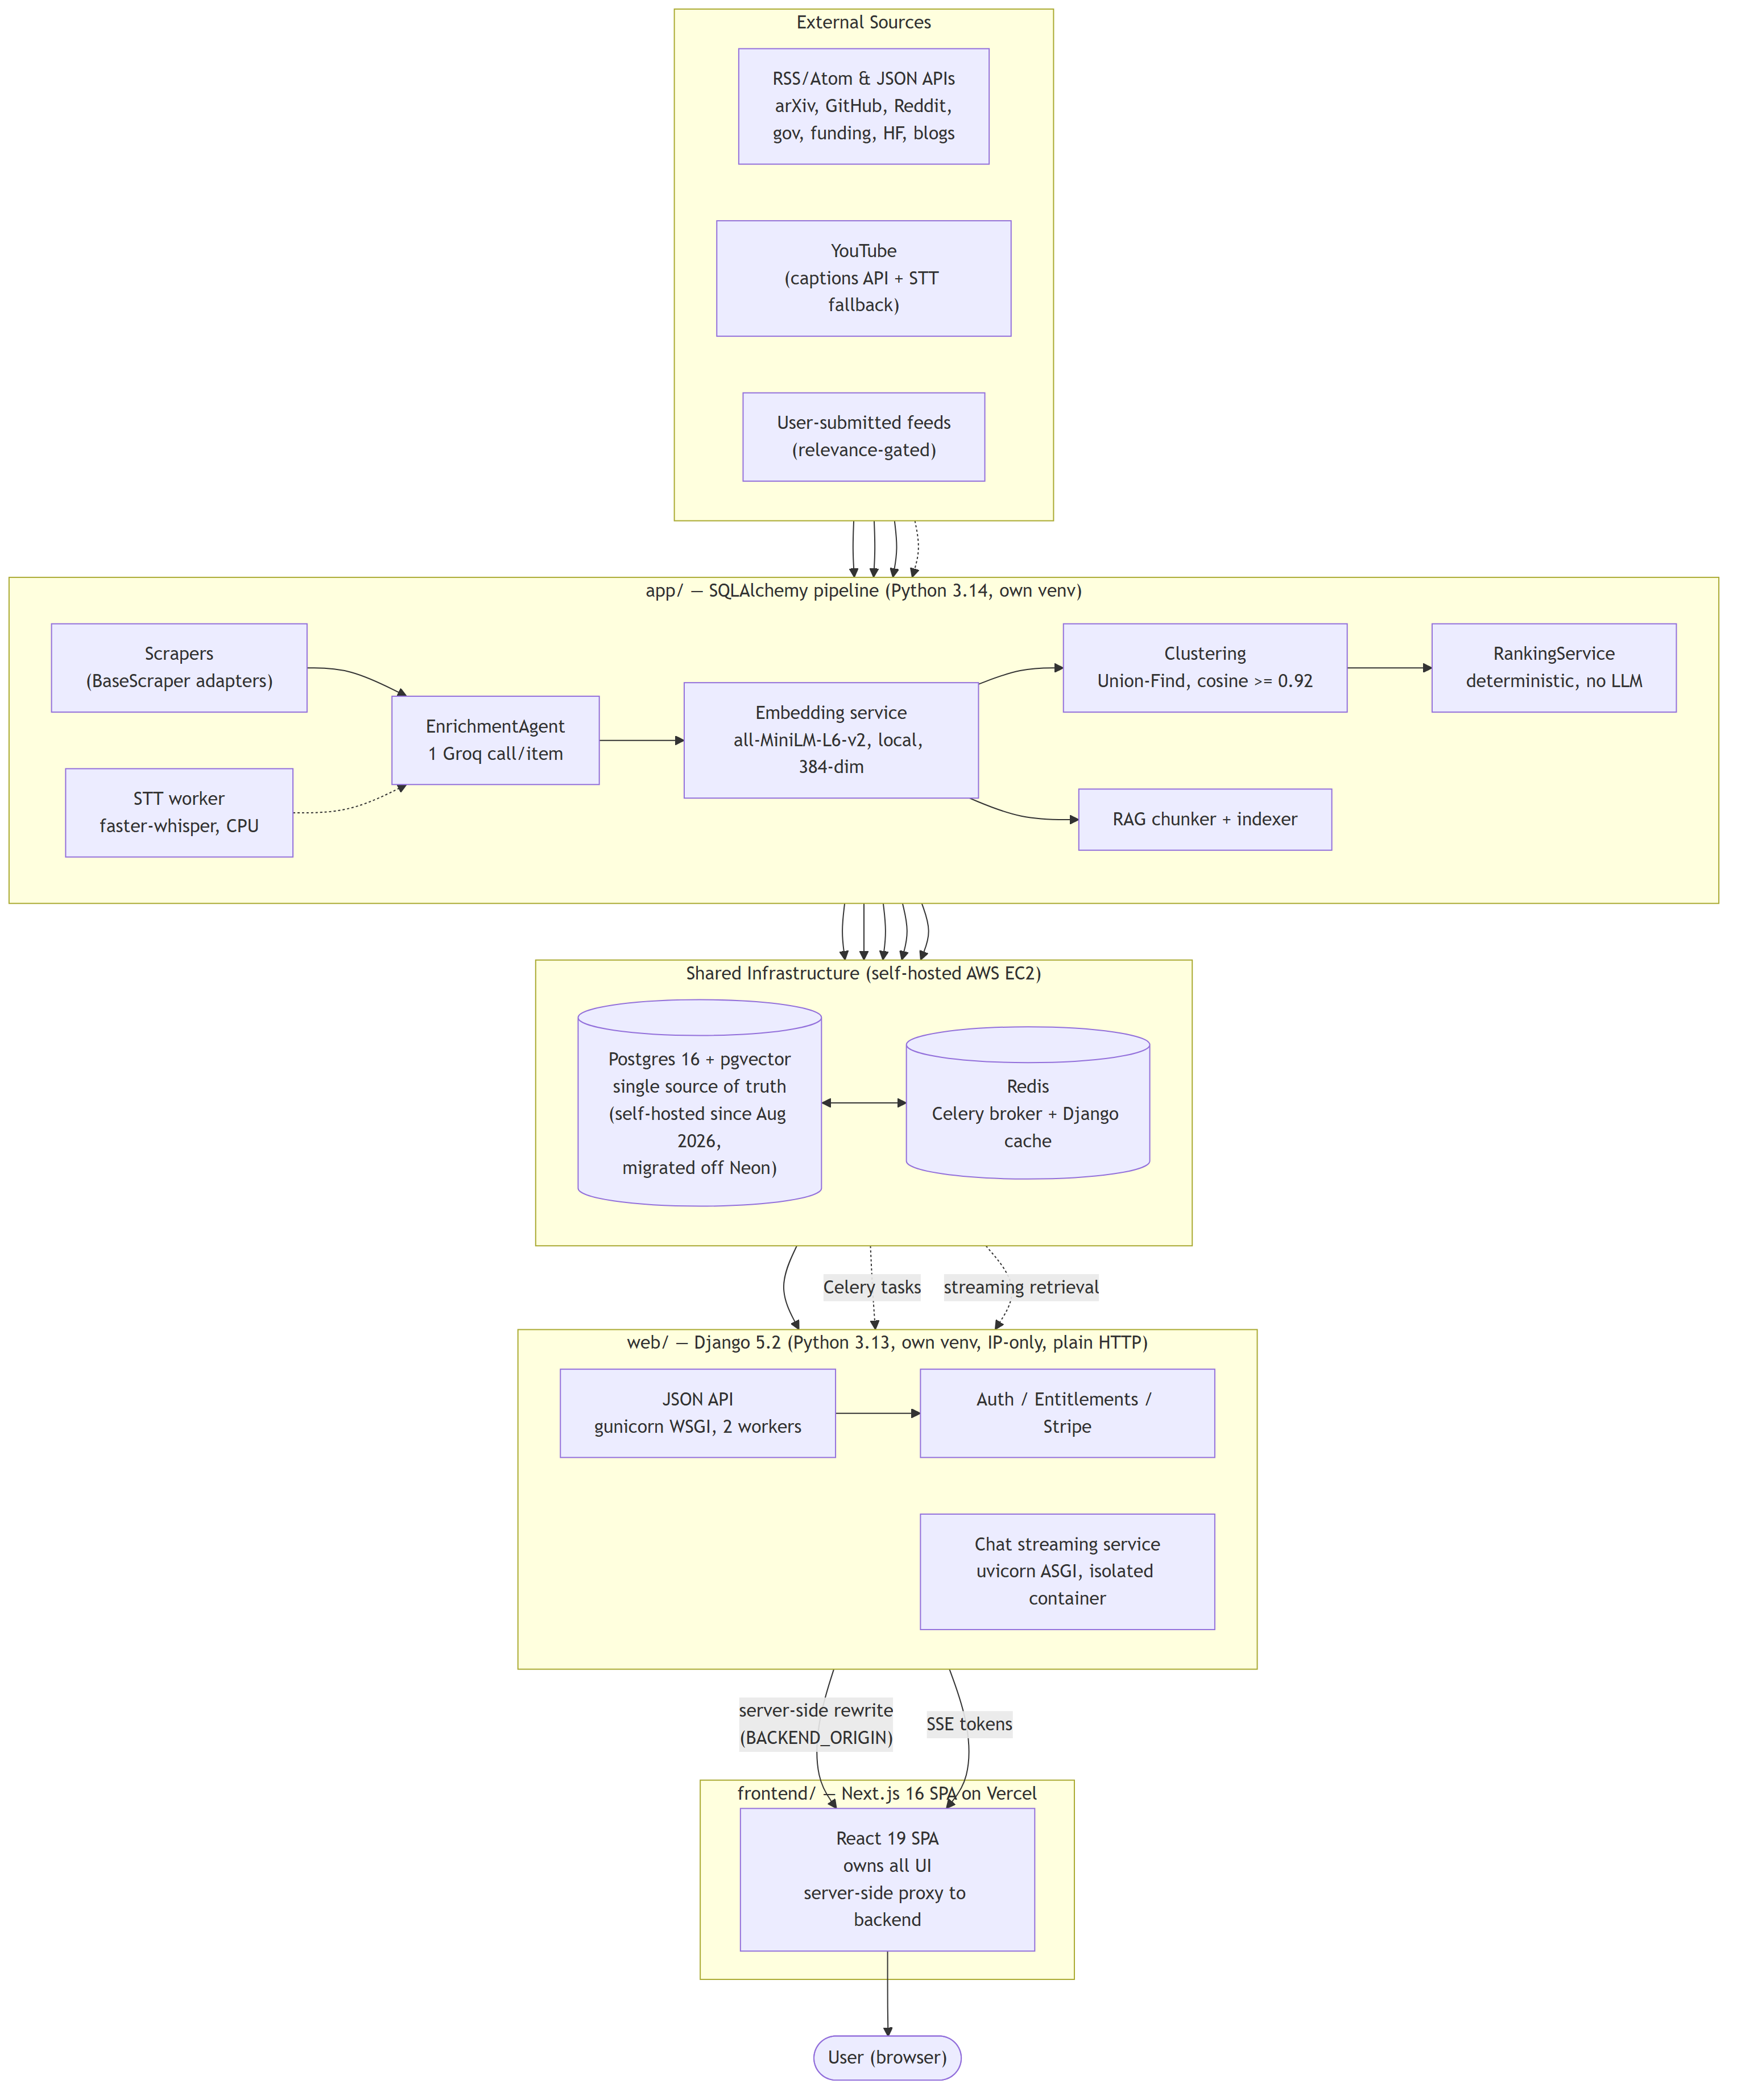
\includegraphics[width=0.85\textwidth,height=0.88\textheight,keepaspectratio]{figures/system_architecture.png}
\caption{AI Compass system architecture: external sources feed the
pipeline, which writes to a shared PostgreSQL+pgvector database; the Django
backend and Next.js frontend serve users, with a dedicated ASGI process
isolating the RAG assistant's SSE streaming from the main WSGI
application.}
\label{fig:sysarch}
\end{figure}

Figure~\ref{fig:sysarch} shows how these pieces fit together end to end. At
the top, \textbf{external sources} enter through three paths: RSS/Atom
feeds and JSON APIs (arXiv, GitHub, Reddit, government notices, funding
announcements, Hugging Face, and blogs), YouTube (captions API first,
speech-to-text fallback otherwise), and user-submitted feeds, gated by the
relevance check before their content is ever ingested. All three feed the
\textbf{pipeline}, whose five stages the figure exposes explicitly:
source-specific \textbf{scrapers} hand raw items to the
\textbf{EnrichmentAgent}, which makes the single structured LLM call per
item; its output is embedded by the local \textbf{embedding service};
embeddings feed both \textbf{clustering}, which groups near-duplicates, and
the \textbf{RAG chunker and indexer}, which builds the passage index the
assistant retrieves from; clustering output finally reaches the
deterministic \textbf{RankingService}. The dashed edge from the
\textbf{STT worker} into the EnrichmentAgent reflects that transcribed
video re-enters the same enrichment step as any other content, rather than
following a separate path.

Everything the pipeline produces is written to the \textbf{shared
infrastructure} box: a self-hosted PostgreSQL~16 instance with
\texttt{pgvector}, and Redis, both on the same AWS EC2 host. Redis serves a
dual role, drawn as one box connected bidirectionally to Postgres: it is
the Celery broker for the pipeline's background tasks and, separately, the
Django cache. From this shared store, the \textbf{Django backend} serves
two distinct kinds of traffic through two distinct processes: the
\textbf{JSON API}, under Gunicorn as a conventional WSGI application with
two synchronous workers, handling authentication, entitlements, Stripe, and
every ordinary request; and a \textbf{dedicated chat streaming service},
the same Django codebase's ASGI entry point under Uvicorn in its own
container. The two reach the shared infrastructure differently (the JSON
API dispatches Celery tasks and waits for a result, while the chat service
issues streaming retrieval calls), and the isolation exists specifically so
a long-lived server-sent-event connection can never occupy one of the JSON
API's only two workers. Finally, the \textbf{Next.js frontend}, on Vercel,
owns the entire UI and reaches the backend over two channels: a server-side
rewrite proxying ordinary API calls same-origin, and a direct SSE token
stream for chat, before rendering to the \textbf{user's browser}.

\section{Key Technology Decisions}
\label{sec:arch-tech-decisions}

Table~\ref{tab:techstack} summarizes the primary technology choices behind
each major layer of the system.

\begin{table}[htbp]
\centering
\caption{Key technology decisions across the three codebases.}
\label{tab:techstack}
\begin{tabular}{|p{3.8cm}|p{11cm}|}
\hline
\textbf{Layer} & \textbf{Choice} \\
\hline
Language / runtime & Python 3.14 (pipeline), Python 3.13 (Django), TypeScript / Next.js 16 (frontend) \\
\hline
Database & PostgreSQL 16 with the \texttt{pgvector} extension \\
\hline
Task queue & Celery with Redis as broker, split into \texttt{default}/\texttt{interactive}/\texttt{stt} queues \\
\hline
LLM provider & Groq (Llama~3.1~8B and Llama~3.3~70B tiers) \\
\hline
Embedding model & \texttt{all-MiniLM-L6-v2}, local, 384-dimensional \\
\hline
ASR & \texttt{faster-whisper} \texttt{distil-large-v3}, CPU-only \\
\hline
\end{tabular}
\end{table}

Each row in Table~\ref{tab:techstack} reflects a trade-off rather than a
default choice. The pipeline and the Django application sit on different,
independently upgradable Python versions because they are separate
deployment units with no shared runtime to reconcile, consistent with
Section~\ref{sec:arch-three-codebases}. PostgreSQL with \texttt{pgvector}
lets ordinary relational data and vector similarity search live in the one
database the cross-ORM boundary already depends on, rather than operating
a second, specialized vector store. Celery with Redis gives the system
three independently tunable queues: a slow speech-to-text job can never
delay the six-hourly batch pipeline, and neither can delay a live
user-facing search or assistant request, expanded on in
Section~\ref{sec:arch-task-orchestration}. Groq was chosen for its
low-latency inference of open-weight models, used at two tiers so
high-volume tasks (per-item enrichment, query condensation) run on the
smaller 8B model while assistant answer generation uses the larger 70B
model. \texttt{all-MiniLM-L6-v2} runs locally at negligible cost, avoiding
a per-call external dependency for an operation every ingested item and
every search query requires. \texttt{faster-whisper}'s
\texttt{distil-large-v3} was chosen as a CPU-only, no-GPU-required speech-
to-text engine, a constraint imposed by the project's deployment budget
rather than a performance-first choice; its measured throughput on that
hardware is reported in the evaluation chapter rather than assumed here.

\section{Background Task Orchestration}
\label{sec:arch-task-orchestration}

All scheduled and asynchronous work in AI Compass runs through Celery, with
work partitioned across three queues chosen to keep unrelated latency and
resource profiles from interfering with one another.

The \textbf{default} queue carries the pipeline's own scheduled work
(scraping, enrichment, embedding, clustering, and ranking) triggered on a
recurring six-hour cycle by Celery's beat scheduler rather than by any user
action. The \textbf{interactive} queue carries work a user is actively
waiting on: semantic search, retrieval for the conversational assistant,
and processing a newly submitted source, all of which need to feel like a
live, synchronous response and are therefore routed away from the default
queue so a long-running pipeline pass cannot delay them. The
\textbf{stt} queue isolates speech-to-text transcription because it is
CPU-heavy and can run for tens of minutes on a single long video; its own
queue and worker mean a transcription in progress never blocks the batch
pipeline or a live request on the interactive queue. This three-way
separation is a direct, mechanical consequence of the non-functional
requirements set out in Section~\ref{sec:req-nonfunctional}: an optional,
slow subsystem must be able to degrade in isolation without degrading the
rest of the system.

\chapter{Data Acquisition and Content Intelligence}
\label{ch:data-pipeline}

The pipeline codebase (\texttt{app/}) is the single point of entry through which every piece of content (a paper, a code release, a video, a government filing, a funding announcement) enters AI Compass. This chapter documents the full path an item travels from external source to a scored, embedded, clustered row in the shared database: how sources are registered and dispatched, how a user-submitted feed is screened before it is trusted, how one language-model call produces the structured intelligence attached to every item, how a deterministic quality score is computed, and how near-duplicate coverage of the same real-world story is detected and merged. Every mechanism described here is a design choice made under the project's governing principle stated in Chapter~1 (\emph{ingest once, personalize later}), so none of the computation in this chapter is user-specific; it runs exactly once per item, globally, regardless of how many users eventually see the result.

\section{Source Registry and Ingestion Adapters}
\label{sec:source-registry}

AI Compass ingests content through a \texttt{sources} database table that currently holds 16 rows. Of these, 9 are dispatched through an adapter registry keyed by a \texttt{source.key} string: \texttt{arxiv}, \texttt{github\_release}, \texttt{youtube}, \texttt{reddit}, \texttt{government\_us}, \texttt{government\_uk}, \texttt{government\_nist}, \texttt{funding\_crunchbase}, and \texttt{huggingface\_model}. A further 2 rows (\texttt{blog\_openai} and \texttt{blog\_anthropic}) are legacy stubs: they exist only as foreign-key anchors so that historical articles retain a valid \texttt{source\_id}, but the registry never dispatches them, because the actual OpenAI and Anthropic blog scraping is performed by a separate, hardcoded \texttt{BlogScraper} that bypasses the registry entirely. The remaining rows are sources that individual users submitted through the product and that passed the relevance gate described in Section~\ref{sec:relevance-gate}.

Every registry-dispatched source is handled through a common adapter interface: an abstract \texttt{BaseScraper} base class defining the scrape-and-persist contract, behind which sit two families of concrete implementation. The first is a single, generic, configuration-driven \texttt{RssFeedScraper} that reads a feed URL and a small set of parsing hints from the source's own database row, so adding a new pure-RSS source requires zero new code: only a new row in \texttt{sources}. The second family consists of five bespoke \texttt{BaseScraper} subclasses, written where the source exposes a structured JSON or REST API rather than an RSS feed and therefore cannot be handled generically: the arXiv API, the GitHub Releases API, the YouTube Data API (paired with transcript retrieval, Chapter~8), the Federal Register API, and the Hugging Face Hub API. This is a deliberate cost-of-extension trade-off: the common RSS case is free to add, while sources whose data model genuinely differs earn their own adapter rather than being force-fitted into a generic one.

\section{User-Submitted Source Screening}
\label{sec:relevance-gate}

Users can propose their own sources, which raises an obvious risk: an unscreened submission could flood the shared content pool with material unrelated to AI, degrading the corpus for every other user. AI Compass gates every user-submitted source behind an automated relevance check before it is admitted into the registry-eligible pool. A deliberate, disclosed design decision governs how this check works: it is \emph{not} a generative-AI judgment call. Routing every submission through a large language model would add both latency and per-submission cost to a request path that a Django worker is synchronously blocked on, for a decision that does not require language understanding at the level an LLM provides.

Instead, the gate is a cheap, deterministic, embedding-similarity heuristic. The candidate feed's most recent items are embedded (using the same embedding model described in Section~\ref{sec:schema}), and the mean cosine similarity between those item embeddings and a corpus centroid is computed, where the centroid is the mean embedding of a 500-row random sample drawn from the existing \texttt{embeddings} table. Let $\bar{s}$ denote this mean similarity. The decision rule is:
\begin{equation}
\label{eq:relevance-gate}
\text{decision}(\bar{s}) =
\begin{cases}
\text{accept} & \text{if } \bar{s} \geq 0.30 \\[2pt]
\text{reject} & \text{if } \bar{s} \leq 0.12 \\[2pt]
\text{keyword fallback} & \text{otherwise}
\end{cases}
\end{equation}
Submissions whose similarity falls in the gray zone between the two thresholds are resolved by a secondary, equally non-generative heuristic that measures the density of AI-related keywords in the candidate items, rather than being defaulted to either outcome. The gate is intentionally conservative at both ends and defers only the ambiguous middle to a second cheap signal, keeping the entire check free of any per-submission LLM inference.

\section{Content Enrichment}
\label{sec:enrichment}

Once an item is ingested and deduplicated (Section~\ref{sec:schema}), it is enriched exactly once by a single structured LLM call on Groq's cheapest tier, \texttt{llama-3.1-8b-instant}, returning a Pydantic-validated output containing a summary, controlled-vocabulary topics, named entities, a \texttt{content\_category} label, a \texttt{technical\_depth} rating (1--5), key points, technical details, a business angle, and a ``why it matters'' statement. This deliberately replaces what would otherwise be four or five separate per-item calls (summarization, topic tagging, entity extraction, category classification, business-relevance) with one round trip: since enrichment runs over every ingested item, not per user, this multiplicative saving in latency and cost is the entire justification.

Because the output is machine-generated and only schema-validated, defensive validation applies rather than trusting it outright: an invalid \texttt{content\_category} falls back to \texttt{"other"}, and any entity or topic failing validation against the controlled vocabulary (Section~\ref{sec:taxonomy}) is silently dropped, never invented. A disclosed limitation: content is truncated to its first \texttt{content[:10000]} characters before the call, so long articles and transcripts are only partially seen, mitigated only for long video via Chapter~8's map-reduce mechanism, while ordinary long articles remain subject to the ceiling.

\section{Quality Scoring}
\label{sec:quality-score}

Independently of enrichment, every item receives a deterministic content-quality score, computed by a fully transparent, project-specific formula rather than a learned model. This score is intentionally not drawn from prior recommender-systems literature; it is an AI Compass project-specific formulation, designed to reward exactly the properties that make an item usable downstream (successfully enriched, substantive in length, entity- and topic-rich, and recent):
\begin{equation}
\label{eq:quality-score}
\begin{split}
\text{score} = {}& 0.30\,\mathbb{1}[\text{enriched}] \;+\; 0.20\,\text{length\_score} \;+\; 0.15\,\min\!\left(1,\tfrac{\text{entity\_count}}{5}\right) \\
& {}+\; 0.15\,\min\!\left(1,\tfrac{\text{topic\_count}}{3}\right) \;+\; 0.20\,\text{freshness}
\end{split}
\end{equation}
where $\mathbb{1}[\text{enriched}]$ is 1 if the item has a valid enrichment record and 0 otherwise, \text{entity\_count} and \text{topic\_count} are the number of validated entities and topics attached to the item, and the two component terms are themselves defined as
\begin{equation}
\label{eq:quality-components}
\text{length\_score} = \min\!\left(1,\ \frac{\ln(1+\text{content\_length})}{\ln(1+5000)}\right), \qquad
\text{freshness} = \exp\!\left(-\frac{\text{age\_days}}{14}\right).
\end{equation}
The logarithmic length term rewards substantive content while saturating near 5,000 characters so that arbitrarily long items are not rewarded without bound; the freshness term is an exponential decay with a 14-day half-life-like constant, so a score computed today already discounts an item that was fresh a month ago. This score is stored per item and is not itself a ranking decision; it is one of the five weighted signals consumed by the personalized ranking formula presented in Chapter~6, where it enters as the \texttt{quality} term.

\section{Taxonomy and Named-Entity Extraction}
\label{sec:taxonomy}

AI Compass classifies content along two structurally different axes. The first is a fixed, controlled taxonomy of exactly 27 topic slugs, curated so that every enrichment call assigns topics only from this closed vocabulary rather than free text. Of these 27 slugs, 15 overlap exactly with the vocabulary exposed to users during onboarding as selectable \texttt{Interest} chips; the remaining 12 are content-classification-only topics, judged too technical or too granular to present as a user-facing preference (for example, distinctions useful for indexing research content but not meaningful as an onboarding choice). This split means the taxonomy serves two audiences at once from a single source of truth: the classification layer that tags every item, and the narrower onboarding vocabulary that a user actually sees.

The second axis is named-entity extraction, which is deliberately open-ended rather than drawn from a fixed list. Entities fall into four types (company, model, person, and technology) and are deduplicated within a type by exact name match, i.e. by the pair (name, entity\_type). This is a disclosed limitation rather than an oversight: because deduplication is purely lexical, two spellings of the same real-world entity, such as "OpenAI" and "Open AI," can coexist as distinct entity rows rather than being merged into one canonical record. Resolving this would require an entity-canonicalization step (for instance, a second embedding-similarity pass over entity names, or a curated alias table) that AI Compass does not currently implement; the trade-off accepted here is that entity extraction stays simple and cheap, at the cost of occasional near-duplicate entities that a future canonicalization pass would need to merge.

\section{Near-Duplicate Clustering}
\label{sec:clustering}

The same real-world event is frequently covered by multiple outlets (a model release reported by both a GitHub changelog and several downstream blog posts, for instance). AI Compass detects this kind of near-duplicate coverage through a purpose-built clustering step, run on a schedule as part of every full pipeline pass rather than incrementally. The mechanism is not a clustering library; it is a hand-rolled Union-Find (disjoint-set) data structure~\cite{tarjan1975unionfind} applied over a k-nearest-neighbor similarity graph built with pgvector. For each embedded item, its top-8 nearest neighbors are retrieved by cosine similarity, and an edge is kept between two items only when their similarity is at or above 0.92; connected components in the resulting graph become clusters. The code's own comments are explicit that this targets near-duplicate \emph{story} deduplication (multiple outlets covering one event), not general topical grouping, which is instead served by the taxonomy of Section~\ref{sec:taxonomy}. The pipeline rebuilds cluster membership wholesale on every run rather than incrementally: existing membership rows are discarded and replaced in full each time, trading recomputation cost for mechanism simplicity.

The 0.92 threshold was arrived at empirically. An earlier version used 0.85, at which the templated, near-identical phrasing of Hugging Face model-card summaries collapsed every model-card item in a run into one spurious $\approx$60-item ``mega-cluster,'' an artifact of the template, not any shared real-world story. The fix combined excluding the Hugging Face model-card source from clustering entirely with raising the threshold to 0.92 for every other source, tightening ``near-duplicate'' enough that superficially similar but substantively different items no longer merge. Algorithm~\ref{alg:clustering} summarizes the procedure.

\begin{algorithm}[htbp]
\caption{Near-duplicate story clustering via Union-Find over a k-NN similarity graph}
\label{alg:clustering}
\KwInput{Embedded content items $I$; neighbor count $k=8$; similarity threshold $\tau=0.92$}
\KwOutput{Cluster assignment (or none) for every item in $I$}
Initialize a disjoint-set structure with one singleton set per item in $I$\;
\ForEach{item $i \in I$}{
  $N_i \leftarrow$ top-$k$ nearest neighbors of $i$ by cosine similarity (pgvector ANN query)\;
  \ForEach{neighbor $j \in N_i$}{
    \If{$\cos(i,j) \geq \tau$}{
      \textsc{Union}$(i,j)$ \tcp*[f]{merge the two disjoint sets}
    }
  }
}
components $\leftarrow$ connected components of the disjoint-set structure\;
discard every component of size 1 (no near-duplicate found)\;
delete all existing cluster-membership rows\;
bulk-insert the surviving components as new cluster-membership rows\;
\end{algorithm}

Figure~\ref{fig:screenshot-trending} shows this mechanism as it surfaces to end users: the Trending Stories page groups items by the connected components Algorithm~\ref{alg:clustering} produces, ranking each story by how many distinct sources cover it and letting the user restrict the view to a 48-hour, 7-day, or 30-day recency window.

\begin{figure}[htbp]
\centering
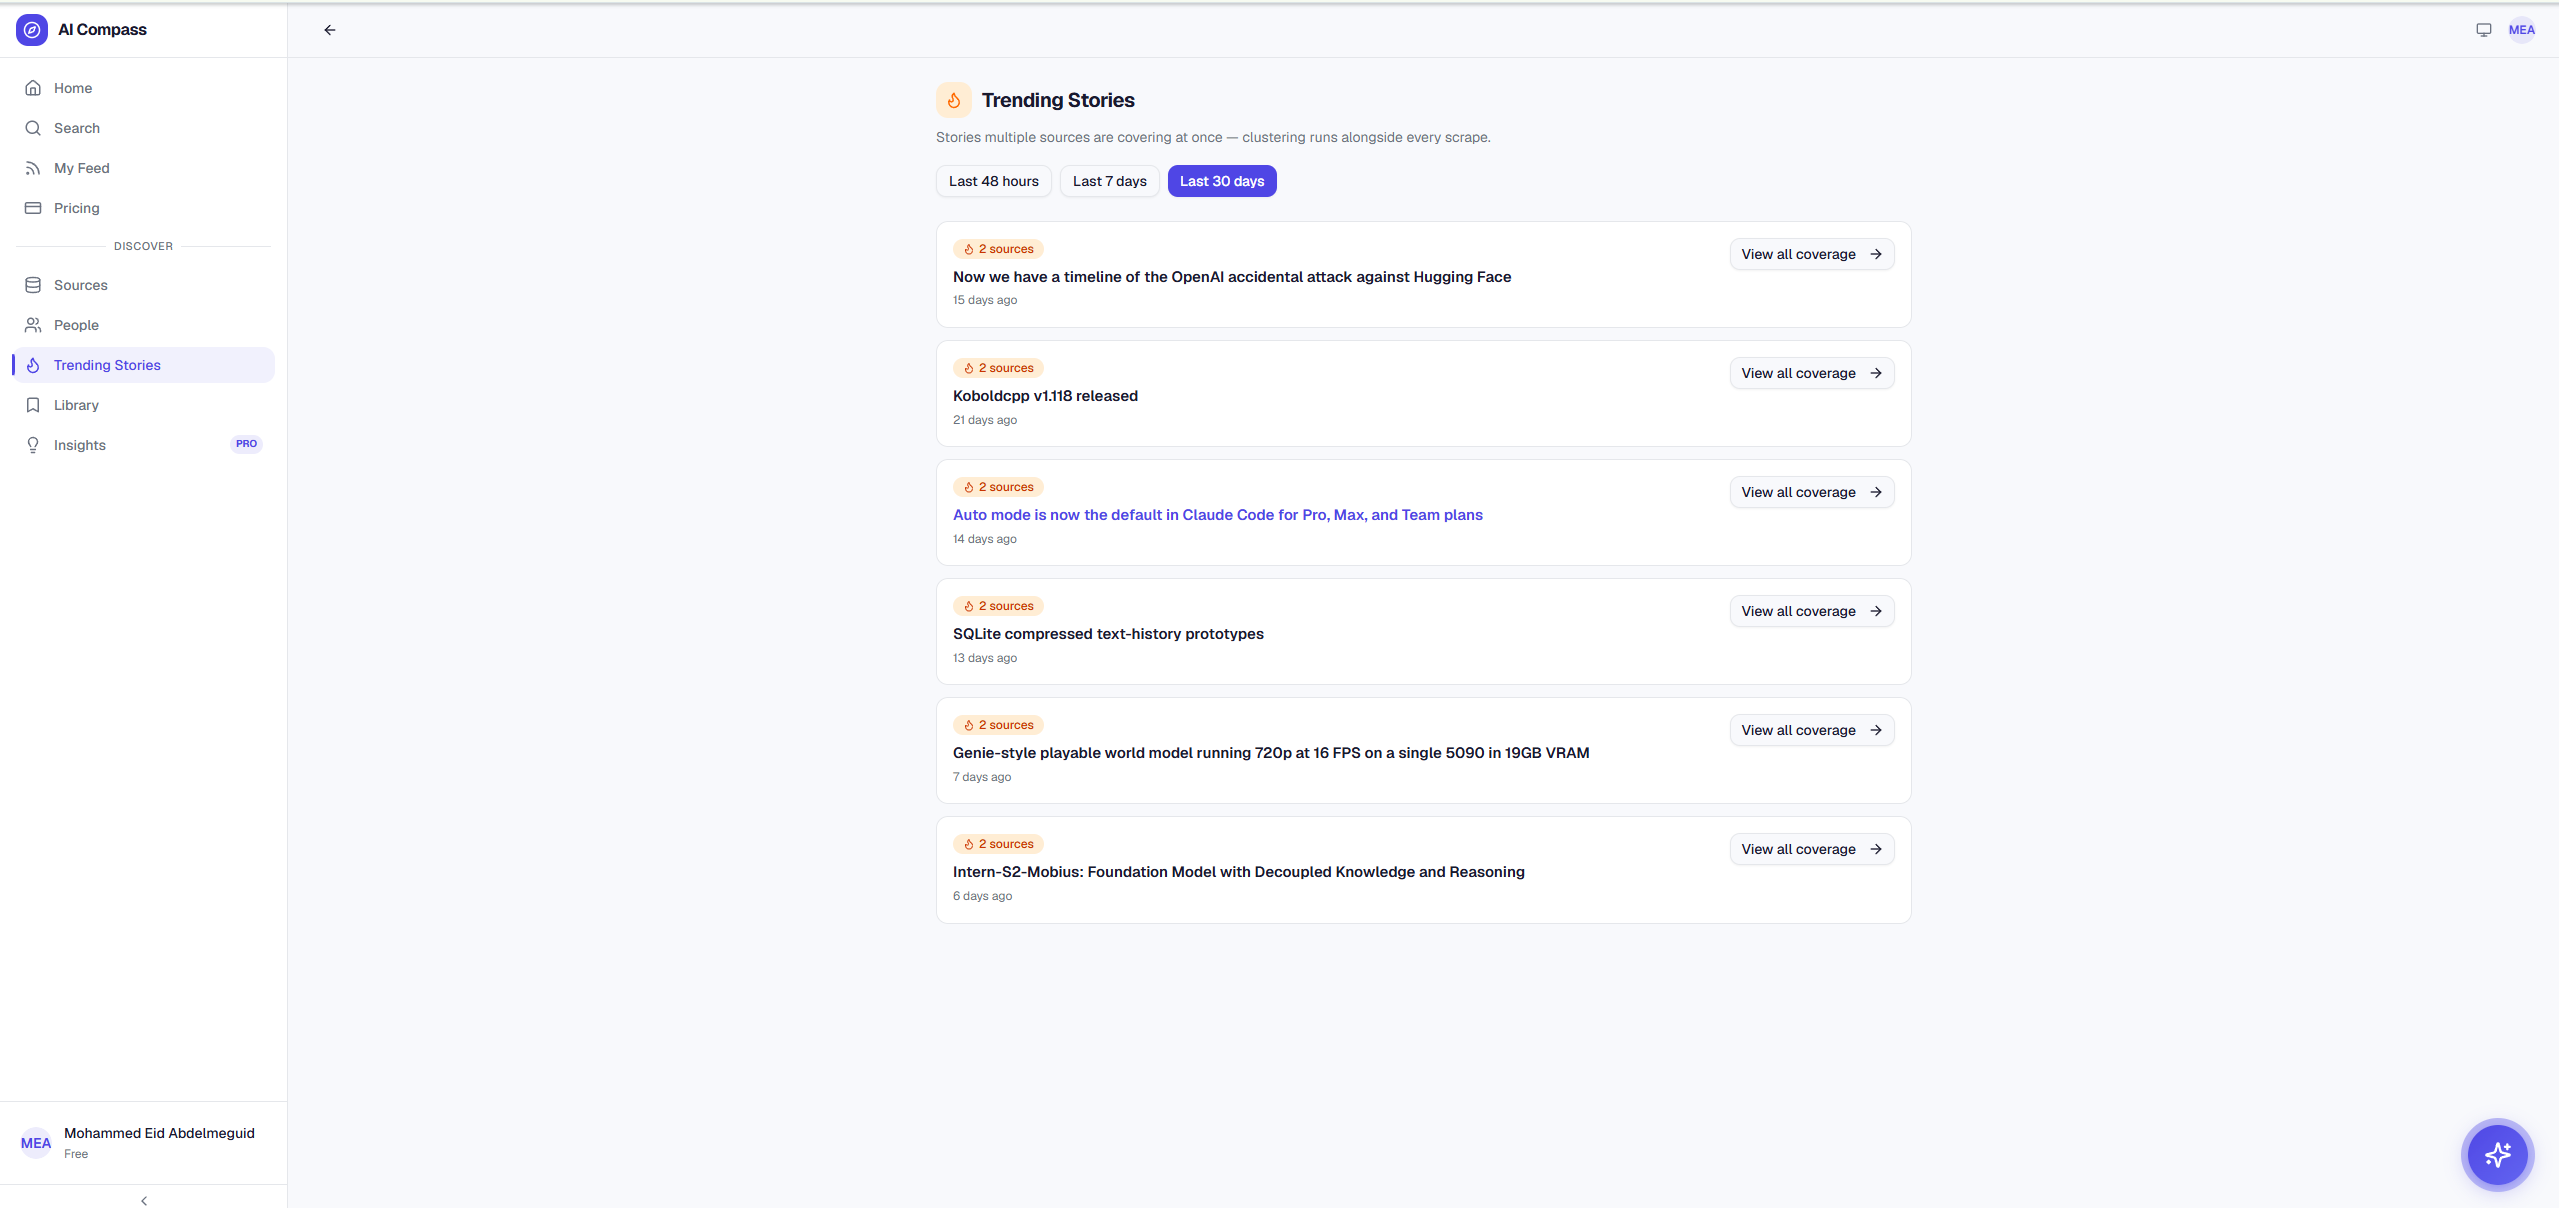
\includegraphics[width=0.85\textwidth]{figures/screenshots/screenshot_trending.png}
\caption{The Trending Stories page, showing near-duplicate story clusters (Section~\ref{sec:clustering}) ranked by the number of distinct sources covering each story, with time-window filters for the last 48 hours, 7 days, and 30 days.}
\label{fig:screenshot-trending}
\end{figure}

\section{Pipeline Data Flow}
\label{sec:pipeline-flow}

Figure~\ref{fig:content-pipeline} lays out the full sequence described in this chapter as a single flow: registry-dispatched and legacy scrapers pull raw items from external sources; ingestion deduplicates and persists them; enrichment attaches the single-call structured intelligence of Section~\ref{sec:enrichment}; embedding computes a vector representation (Section~\ref{sec:schema}); clustering and quality scoring run over the resulting pool; and the passage-level RAG index described in Chapter~7 is populated from the same enriched content. Every stage in this diagram runs once, globally, consistent with the ingest-once-personalize-later principle; none of it is re-triggered by a user viewing content.

\begin{figure}[htbp]
\centering
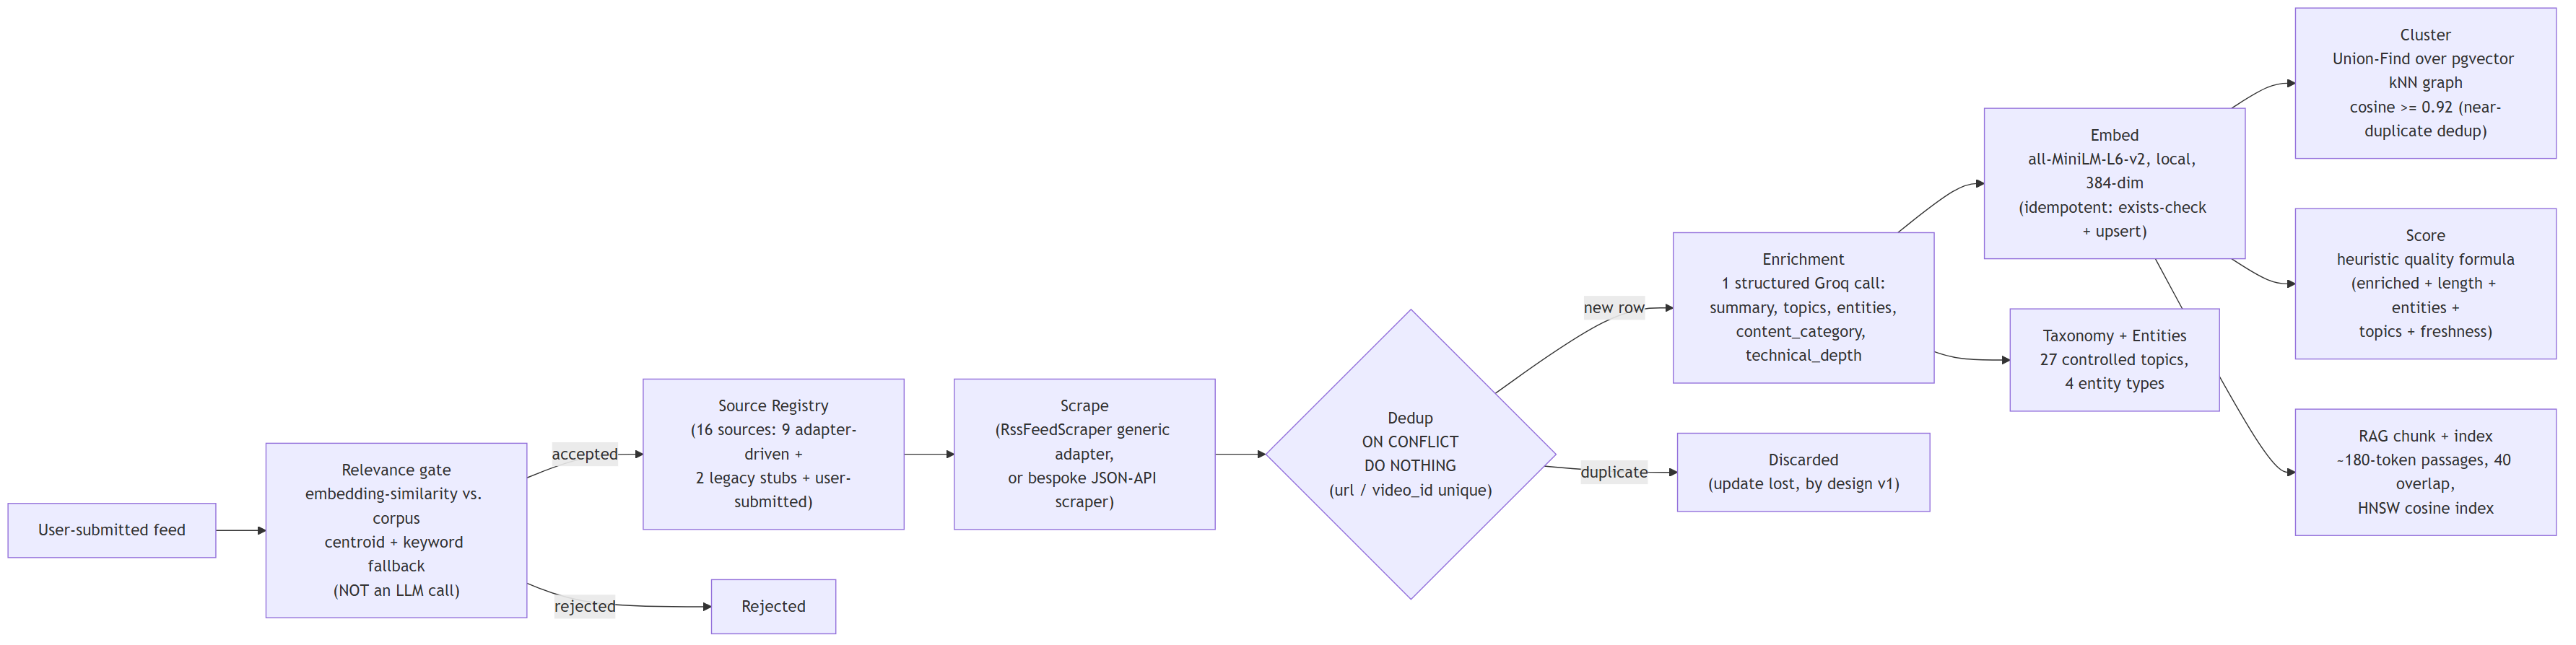
\includegraphics[width=\textwidth,height=0.88\textheight,keepaspectratio]{figures/content_pipeline.png}
\caption{Content ingestion and intelligence pipeline: from source registry through scraping, deduplication, enrichment, embedding, clustering, scoring, and RAG indexing.}
\label{fig:content-pipeline}
\end{figure}

\section{Database Schema}
\label{sec:schema}

The pipeline owns its schema directly through SQLAlchemy, independent of the Django backend's own models (the ownership boundary between the two is formalized in Chapter~4). Figure~\ref{fig:pipeline-schema} shows the pipeline-owned entity-relationship diagram. \texttt{Sources} is the registry table described in Section~\ref{sec:source-registry}; each source's raw items land in \texttt{Articles} or \texttt{YoutubeVideos} depending on content type. Ingestion-time deduplication is enforced at the database level through an \texttt{INSERT ... ON CONFLICT DO NOTHING} clause keyed on a natural unique identifier (the article URL, or the YouTube \texttt{video\_id}), a deliberate v1 design choice that keeps ingestion cheap and idempotent: re-running a scrape never produces duplicate rows. The disclosed cost of this choice is that if a source later republishes a corrected or expanded version of the same URL, that later version is never re-ingested, since the conflict clause silently discards it rather than updating the existing row; this is a genuine limitation of the current design, not an unnoticed bug.

\texttt{ContentEnrichment} stores the structured output of Section~\ref{sec:enrichment}, one row per item, linked polymorphically by a \texttt{(content\_type, content\_id)} pair so the same table serves both articles and videos. \texttt{Embeddings} stores one 384-dimensional vector per item, computed locally with \texttt{all-MiniLM-L6-v2} from the Sentence-BERT / \texttt{sentence-transformers} family~\cite{reimers2019sentencebert,wang2020minilm,sbert_docs}, chosen because it runs locally with no per-embedding API cost, unlike the enrichment LLM call. Every embedding write is idempotent by construction: gated first by an application-level existence check, then independently by a database-level unique constraint on \texttt{(content\_type, content\_id)} enforced through an \texttt{INSERT ... ON CONFLICT DO UPDATE} clause, so duplicate embedding rows are structurally impossible even under a race condition, not merely unlikely. \texttt{RagChunks} is the passage-level index the retrieval-augmented assistant of Chapter~7 queries against; \texttt{ContentClusters} and its membership table record the output of Section~\ref{sec:clustering}; \texttt{ContentScores} stores the quality score of Section~\ref{sec:quality-score}; and \texttt{Entities} / \texttt{TaxonomyTopics} store the two classification axes of Section~\ref{sec:taxonomy}. \texttt{UserRankings}, \texttt{UserAffinities}, and \texttt{UserProfileVectors}, consumed by the ranking mechanism of Chapter~6, were added in a later milestone and are the only tables here that are genuinely per-user rather than global.

\begin{figure}[htbp]
\centering

\includegraphics[width=\textwidth,height=0.88\textheight,keepaspectratio]{figures/pipeline_schema.png}
\caption{Entity-relationship diagram of the pipeline-owned (SQLAlchemy) database schema, including the passage-level RAG index (\texttt{rag\_chunks}) and personalization tables (\texttt{user\_rankings}, \texttt{user\_affinities}, \texttt{user\_profile\_vectors}) added in later milestones.}
\label{fig:pipeline-schema}
\end{figure}

\section{Ingestion Sources Table}
\label{sec:sources-table}

Table~\ref{tab:sources} summarizes the composition of the 16-row \texttt{sources} table, grouped by how each row reaches the content pool: the 9 sources dispatched through the adapter registry, the 2 legacy stub rows, and the remaining user-submitted sources that were admitted through the relevance gate of Section~\ref{sec:relevance-gate}.

\begin{table}[htbp]
\centering
\caption{Composition of the \texttt{sources} registry table (16 rows total).}
\label{tab:sources}
\small
\begin{tabular}{|p{2.3cm}|p{3.4cm}|p{4.4cm}|p{2.6cm}|}
\hline
\textbf{Category} & \textbf{Registry key} & \textbf{Adapter type} & \textbf{Dispatch status} \\
\hline
Research literature & \texttt{arxiv} & Bespoke (arXiv API) & Registry-dispatched \\
\hline
Open-source releases & \texttt{github\_\allowbreak release} & Bespoke (GitHub Releases API) & Registry-dispatched \\
\hline
Long-form video & \texttt{youtube} & Bespoke (YouTube Data API + transcripts) & Registry-dispatched \\
\hline
Developer community & \texttt{reddit} & Generic \texttt{RssFeedScraper} & Registry-dispatched \\
\hline
Government (US) & \texttt{government\_\allowbreak us} & Bespoke (Federal Register API) & Registry-dispatched \\
\hline
Government (UK) & \texttt{government\_\allowbreak uk} & Generic \texttt{RssFeedScraper} & Registry-dispatched \\
\hline
Government (NIST) & \texttt{government\_\allowbreak nist} & Generic \texttt{RssFeedScraper} & Registry-dispatched \\
\hline
Funding \& investment & \texttt{funding\_\allowbreak crunchbase} & Generic \texttt{RssFeedScraper} & Registry-dispatched \\
\hline
Model databases & \texttt{huggingface\_\allowbreak model} & Bespoke (Hugging Face Hub API) & Registry-dispatched \\
\hline
Legacy blog scraping & \texttt{blog\_openai}, \texttt{blog\_\allowbreak anthropic} & Hardcoded \texttt{BlogScraper} & Inert FK-only stubs; bypasses registry \\
\hline
User-submitted & (varies) & Generic \texttt{RssFeedScraper} & Admitted via relevance gate \\
\hline
\end{tabular}
\end{table}

Once admitted, a user-submitted row is scraped through the same generic \texttt{RssFeedScraper} used by any other RSS-based registry source, with no separate code path distinguishing it from one that AI Compass shipped with by default.

Figure~\ref{fig:screenshot-sources} shows the Sources page that exposes Table~\ref{tab:sources}'s registry to the end user: every registry-dispatched source listed with a per-user visibility toggle, the category filter chips corresponding to each row's grouping, and the submission form through which a new user-supplied RSS or YouTube feed enters the relevance gate of Section~\ref{sec:relevance-gate}.

\begin{figure}[htbp]
\centering
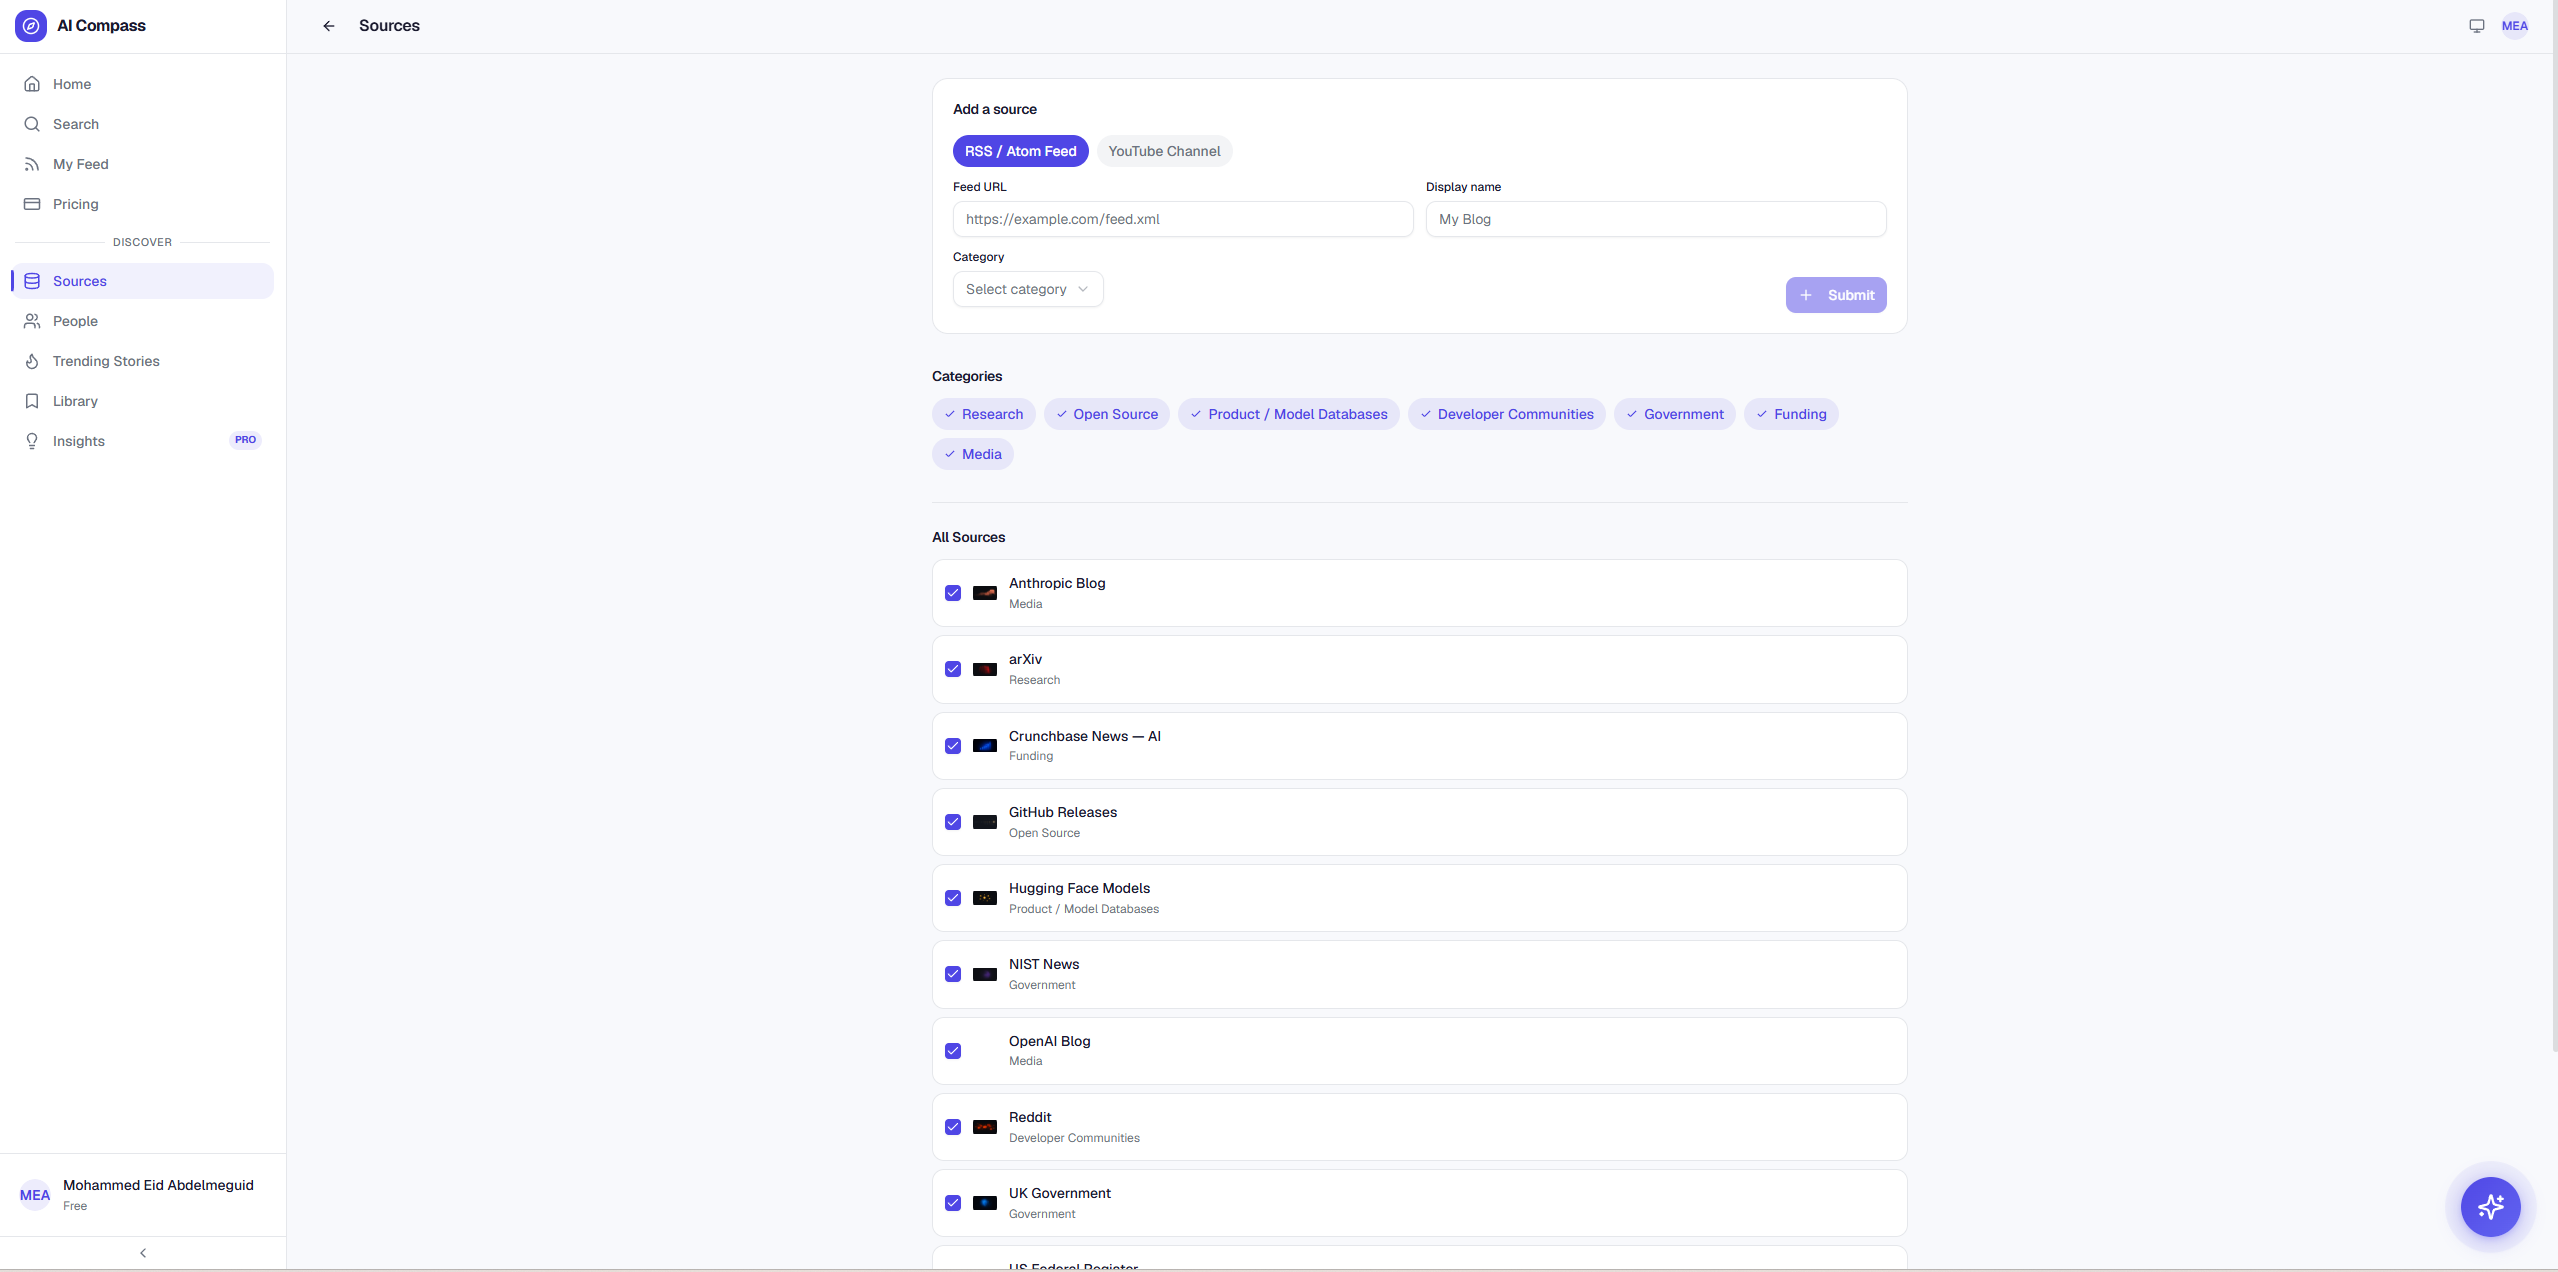
\includegraphics[width=0.85\textwidth]{figures/screenshots/screenshot_sources.png}
\caption{The Sources page, listing the registry-dispatched sources of Table~\ref{tab:sources} with per-user visibility toggles, category filters, and the submission form feeding the relevance gate (Section~\ref{sec:relevance-gate}).}
\label{fig:screenshot-sources}
\end{figure}

\chapter{Personalization and Recommendation}
\label{ch:recommendation}

\section{Overview and Two Ranking Systems}
\label{sec:rec-overview}

AI Compass contains two ranking mechanisms that must be kept conceptually separate. The first, and the subject of most of this chapter, is the \emph{personalized feed ranking} (\texttt{app/services/ranking\_service.py}'s \texttt{RankingService}), which drives a logged-in user's Home feed and digest email: given a content pool and a specific user, it produces a per-user ordered list with a human-readable explanation for every item. The module declares \texttt{RANKER\_VERSION = "v1-deterministic"}, and its own comment calls it ``a documented, heuristic v1, NOT tuned'': fully deterministic (identical inputs always produce identical scores), but its weights, multipliers, and diversification parameter were set by engineering judgement rather than fit to data.

The second mechanism is a considerably simpler, entirely \emph{non-personalized} formula powering the public Home feed shown to a signed-out visitor (\texttt{web/apps/news/feed\_ranking.py}). It shares no code, weights, or behavioral inputs with the personalized ranker; Section~\ref{sec:rec-public-feed} treats it separately so the two are never conflated.

The personalized ranker is a three-stage pipeline followed in order below: \emph{candidate generation} (Section~\ref{sec:rec-candidates}) assembles a bounded eligible pool; \emph{scoring} (Section~\ref{sec:rec-score}) assigns each candidate a deterministic score from five weighted signals adjusted by bounded multipliers; and \emph{selection} (Section~\ref{sec:rec-mmr}) greedily builds the final list under a diversity objective plus a reserved exploration slice. Every selected item receives a templated, non-generative explanation (Section~\ref{sec:rec-explanations}). Section~\ref{sec:rec-pipeline} recaps the pipeline as a figure; Sections~\ref{sec:rec-deferred}--\ref{sec:rec-limitations} close with what was deliberately left out of scope and what was not.

\section{Behavioral Signal Aggregation}
\label{sec:rec-signals}

Personalization begins with raw behavioral events. AI Compass records six event types against a user and a content item: \texttt{impression}, \texttt{click}, \texttt{save}, \texttt{hide}, \texttt{dwell} (time spent on an item), and \texttt{digest\_click} (a link opened from a digest email). These events are the only input to two nightly-recomputed structures that the personalized ranker later reads: \texttt{UserAffinity}, a per-user set of decaying weights along three dimensions (\texttt{topic}, \texttt{source}, and \texttt{entity}), and \texttt{UserProfileVector}, a single per-user embedding summarizing the content the user has actually engaged with.

Both structures are built from the same nightly job over a rolling 90-day window of events, and both apply the same exponential recency decay, with a half-life of 14 days, to each event before it contributes to the aggregate:

\begin{equation}
\text{weight}(u, d) = \sum_{e \,\in\, E_u(d)} w(e) \cdot e^{-\lambda \cdot \text{age\_days}(e)}, \qquad \lambda = \frac{\ln 2}{14}
\label{eq:affinity-decay}
\end{equation}

\noindent where $E_u(d)$ is the set of events belonging to user $u$ associated with dimension value $d$ (a topic, source, or entity), $w(e)$ is a fixed weight per event type, and $\text{age\_days}(e)$ is the event's age at aggregation time. With $\lambda = \ln 2/14$, an event's contribution is exactly halved every 14 days without reinforcement, so recent behavior dominates while older behavior fades smoothly rather than being discarded at a fixed cutoff.

The event-type weights $w(e)$ are asymmetric by design: \texttt{impression} $= 0.1$, \texttt{click} $= 1.0$, \texttt{save} $= 3.0$, \texttt{digest\_click} $= 1.5$: a save counts as a substantially stronger interest signal than a click, and a click stronger than a mere impression. \texttt{hide} is deliberately \emph{negative}, $-2.0$: an explicit rejection actively pulls the corresponding affinity downward rather than merely failing to reinforce it. \texttt{dwell} is folded in as an additional graded engagement signal.

\texttt{UserProfileVector} is built from the same 90-day window, but over a narrower subset of events: only \texttt{click}, \texttt{save}, \texttt{dwell}, and \texttt{digest\_click} contribute, while \texttt{impression} and \texttt{hide} are excluded. It is a decayed, weighted mean of the embeddings behind those qualifying events, L2-normalized before storage so it can be compared to candidate embeddings by cosine similarity. The job wholesale-recomputes this vector nightly rather than updating it incrementally, so it always reflects the exact current 90-day window with no accumulated online-update drift.

\section{Candidate Generation}
\label{sec:rec-candidates}

Before any item can be scored for a given user, it must first survive an \emph{eligibility filter} and then be admitted into a bounded \emph{candidate pool} through one of three routes. The eligibility filter is applied first and is a hard gate, not a scoring adjustment: an item is dropped outright if its source has been excluded by the user, if its content category has been excluded by the user, or if it belongs to a source whose visibility is \texttt{user}-restricted and the requesting user is not subscribed to it. Only items that survive this filter are eligible to enter the candidate pool through any of the three legs described below.

The three legs are a union, not alternatives: an item qualifying through more than one leg is still scored once. \emph{Leg A (recency)} contributes the newest 300 eligible items by \texttt{published\_at}, giving every pool a baseline of current content. \emph{Leg B (similarity)} performs a pgvector nearest-neighbor search against the user's \texttt{UserProfileVector} (Section~\ref{sec:rec-signals}), returning up to 150 closest items by embedding; with no profile vector yet (cold start), it falls back to items whose topic overlaps the user's onboarding interests. \emph{Leg C (follows)} guaranteedly admits any item matching a followed topic, entity, source, or followed person's footprint (blog, GitHub, or YouTube channel); it is the only leg that bypasses recency and similarity entirely, so an old item from a followed source is still admitted. The union is capped at 300 candidates before scoring.

Leg C is also the one place where the platform's Free/Pro entitlement distinction touches candidate generation, and it is worth stating precisely how: a Free-plan user is limited to \texttt{FREE\_FOLLOW\_LIMIT} = 20 follow relationships, while a Pro-plan user may hold an unlimited number. This limit bounds how many items \emph{can possibly} enter through Leg C for a Free user; it does not alter the scoring formula, the multipliers, or the diversification step in any way for either plan. There is no Free/Pro branch anywhere inside the scoring logic itself; the only interaction between entitlements and ranking is this indirect, upstream effect on how much material a Free user's follows can guarantee into the candidate pool before scoring ever begins.

Algorithm~\ref{alg:candidates} summarizes the process.

\begin{algorithm}[htbp]
\DontPrintSemicolon
\KwInput{user $u$, eligible content pool $P$ (after the eligibility filter)}
\KwOutput{candidate pool $C$, $|C| \le 300$}
$A \leftarrow$ top 300 items of $P$ ordered by $\text{published\_at}$ descending\tcp*{Leg A: recency}
\If{$u$ has a stored \texttt{UserProfileVector} $v_u$}{
  $B \leftarrow$ top 150 items of $P$ by cosine similarity to $v_u$ (pgvector ANN search)\tcp*{Leg B: similarity}
}
\Else{
  $B \leftarrow \{\, p \in P : \text{topic}(p) \in \text{onboarding\_interests}(u) \,\}$\tcp*{Leg B cold-start fallback}
}
$F \leftarrow \{\, p \in P : p \text{ matches a followed topic, entity, source, or followed-person footprint} \,\}$\tcp*{Leg C: follows}
$C \leftarrow A \cup B \cup F$, retaining every item in $F$ and truncating $A \cup B$ as needed to cap $|C|$ at 300\;
\Return{$C$}
\caption{Candidate generation (three-leg union)}
\label{alg:candidates}
\end{algorithm}

Figure~\ref{fig:screenshot-preferences} shows the standalone Preferences page that supplies the \texttt{onboarding\_interests}(u) set used by Leg B's cold-start fallback above: a user who has not yet accumulated enough behavioral history for a \texttt{UserProfileVector} instead has their candidate pool shaped directly by the topic chips selected here.

\begin{figure}[htbp]
\centering
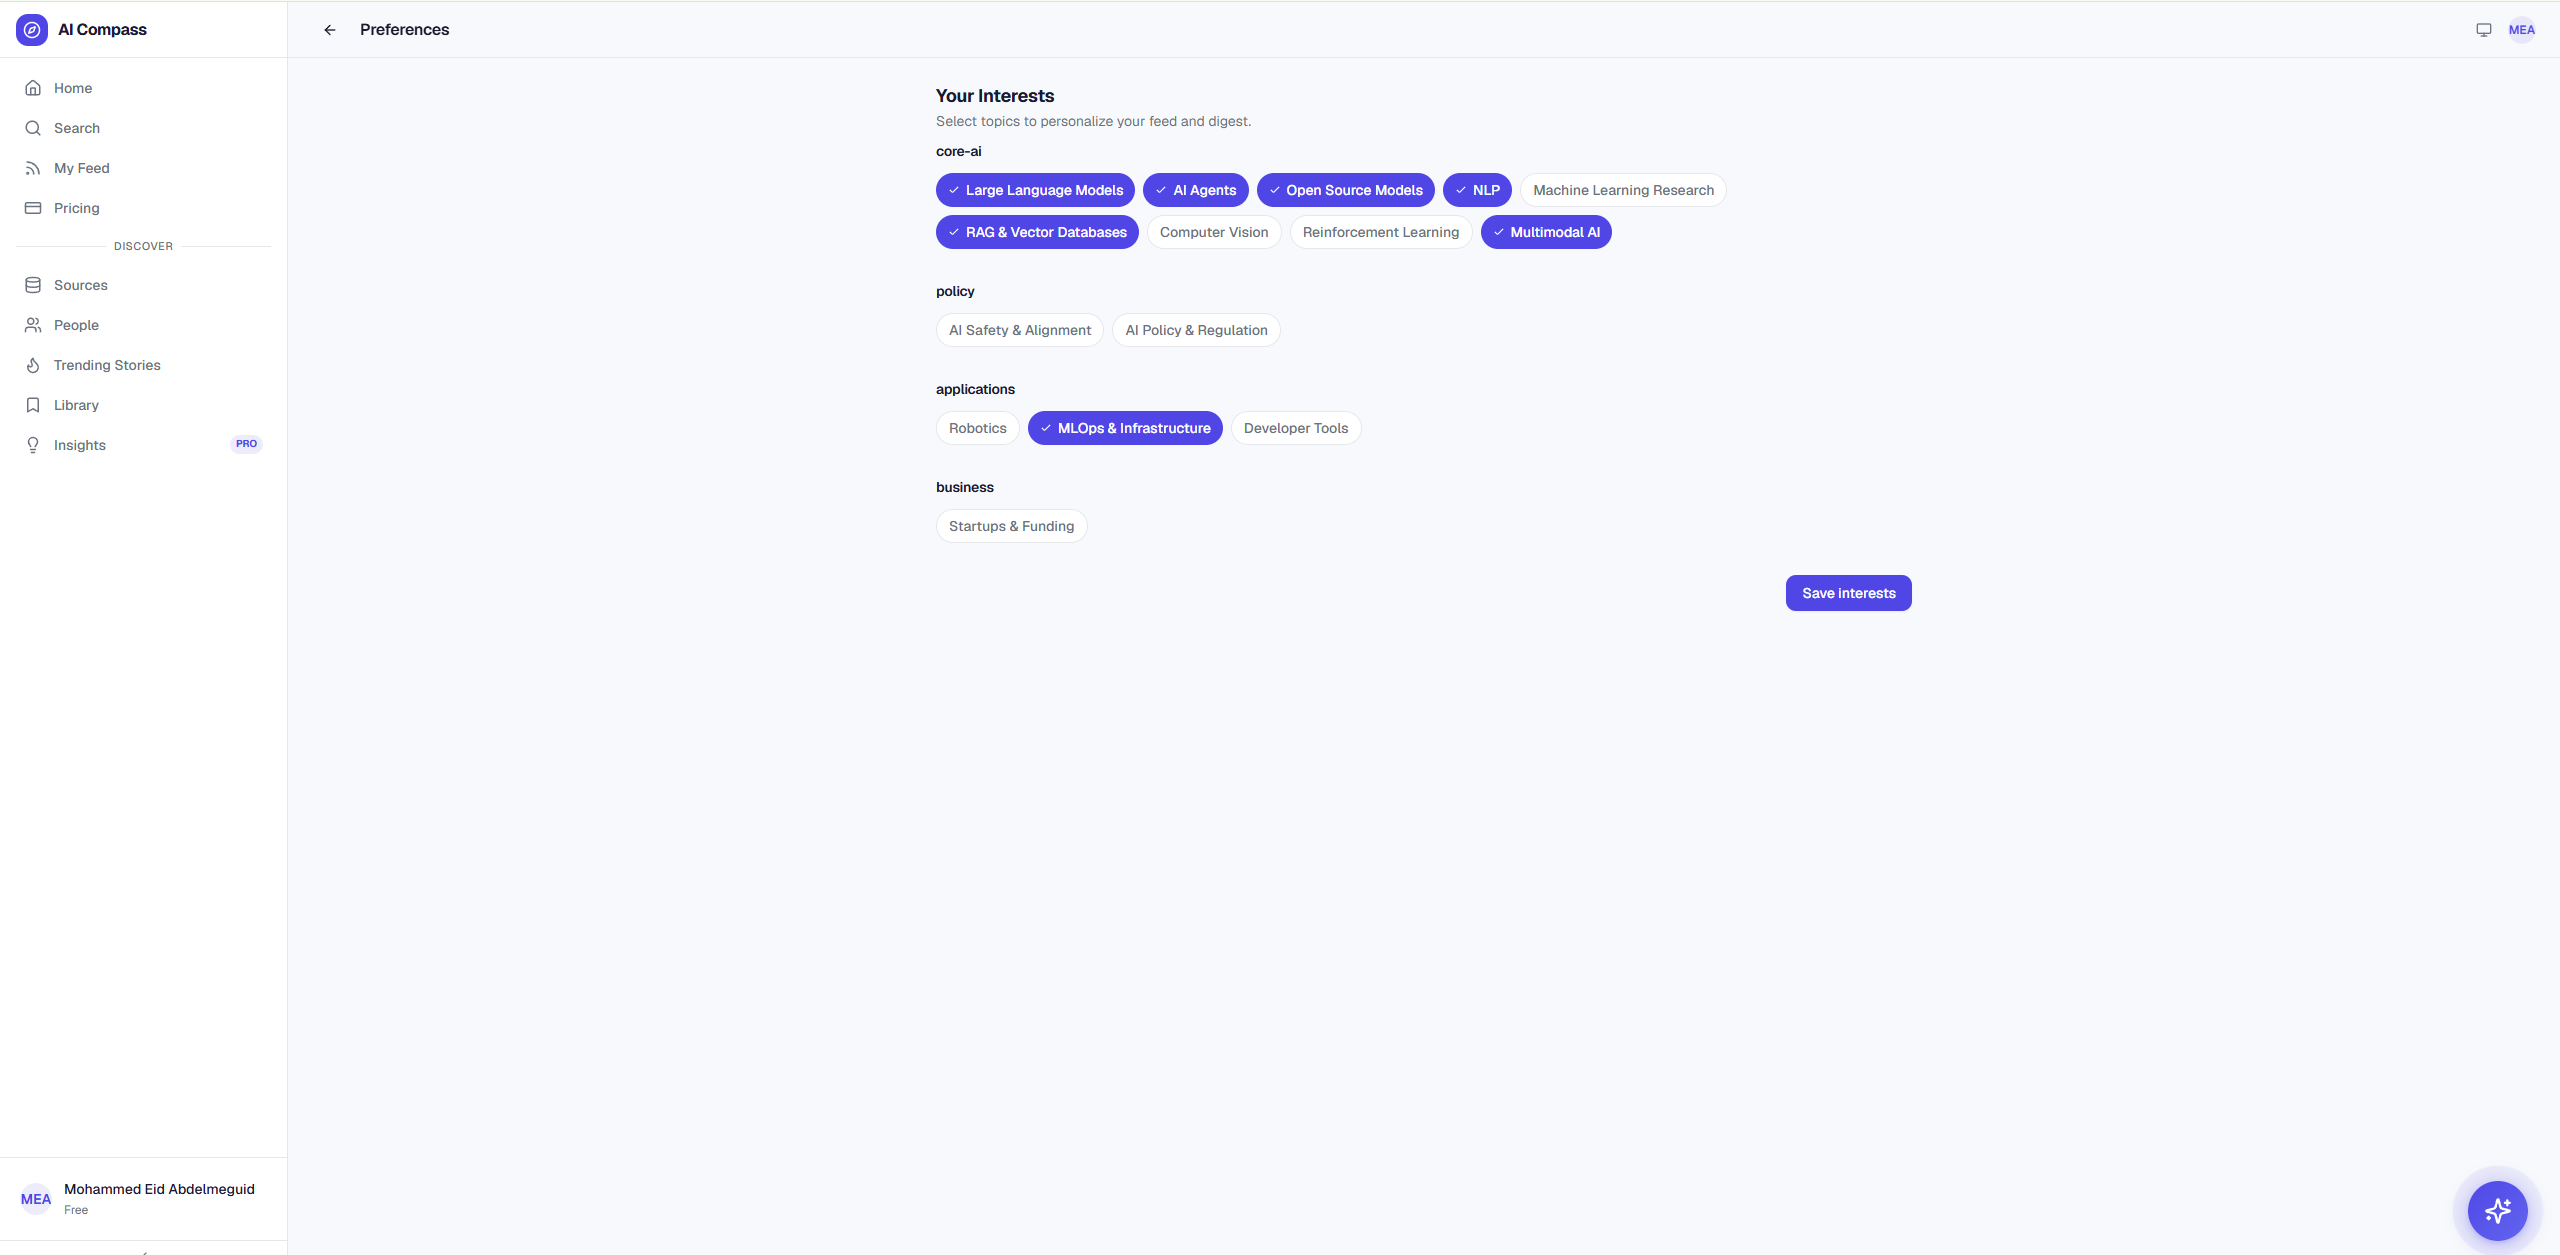
\includegraphics[width=0.85\textwidth]{figures/screenshots/screenshot_preferences.png}
\caption{The Preferences page, showing the interest-selection chip grid that seeds a new user's cold-start candidate generation (Leg B fallback, Section~\ref{sec:rec-candidates}).}
\label{fig:screenshot-preferences}
\end{figure}

\section{The Personalized Ranking Score}
\label{sec:rec-score}

Once a bounded candidate pool exists for a user, every candidate is scored by \texttt{RankingService.\_score()}. The score is built in three steps, expressed here as three equations, all implemented in the same function.

\begin{equation}
\text{base} = 0.35\,I + 0.20\,Q + 0.15\,F + 0.15\,S + 0.15\,N
\label{eq:ranking-base}
\end{equation}

\begin{itemize}
  \item $I$ (\emph{interest\_score}): the candidate's maximum per-topic \texttt{UserAffinity} weight (dimension \texttt{topic}), normalized by the user's own maximum topic-affinity weight, so that $I \in [0,1]$ regardless of how large or small a user's absolute affinity magnitudes are. If the user has no affinity data at all, a cold-start fallback applies: $I = 1.0$ if the item shares a topic with the interests the user selected during onboarding, and $I = 0.0$ otherwise.
  \item $Q$ (\emph{quality}): read directly from the \texttt{content\_scores.score} value, a separate quality heuristic computed once per item by the content-intelligence pipeline (Chapter~5) and never recomputed here; it defaults to $0.5$ if no score row yet exists for the item.
  \item $F$ (\emph{freshness}): $F = \exp\!\left(-\dfrac{\ln 2}{48}\cdot\text{age\_hours}\right)$, an exponential decay with a 48-hour half-life measured from the item's publication time to the present.
  \item $S$ (\emph{source\_affinity}): the item's per-source \texttt{UserAffinity} weight, normalized by the user's own maximum source-affinity weight in the same way as $I$; it defaults to $0.5$ if the user has no source-affinity data at all.
  \item $N$ (\emph{novelty}): $N = 1.0$ if the item has never been shown to this user, determined by a 30-day lookback over digest-email click tokens; otherwise $N = 1 - \exp\!\left(-\dfrac{\ln 2}{10}\cdot\text{age\_days}\right)$, a recovery curve with a 10-day half-life, where $\text{age\_days}$ is the time since the item was last shown. This is an important precision point: because ``shown'' is tracked exclusively through digest-email click tokens, $N$ in the current implementation measures ``has this item not recently been emailed to this user,'' not ``has this item not recently been viewed anywhere, including the web feed.'' A user who has already seen and read an item on the web feed, but never received it in a digest email, is still scored as though the item were fully novel, a real, disclosed precision gap rather than an intended design property, revisited in Section~\ref{sec:rec-limitations}.
\end{itemize}

The weighted sum in Equation~\ref{eq:ranking-base} is the largest single design decision AI Compass makes about what personalization means in this system: 35\% of the score rewards demonstrated topical interest, 20\% rewards independently assessed content quality, and the remaining 45\% is split evenly across recency, source loyalty, and novelty. These five weights are a project-specific configuration choice, not a value drawn from prior literature.

\begin{equation}
\text{final\_score} = \text{clamp}_{[0,1]}\Bigl(\text{base} \times M_{\text{depth}} \times M_{\text{format}} \times M_{\text{lean}} \times M_{\text{time}}\Bigr)
\label{eq:ranking-final}
\end{equation}

\begin{itemize}
  \item $M_{\text{depth}}$ compares the item's \texttt{content\_enrichment.technical\_depth} classification against the band implied by the user's stated expertise level.
  \item $M_{\text{format}}$ favors video or article content according to the user's stated format preference.
  \item $M_{\text{lean}}$ favors research-leaning or industry-leaning content according to the user's stated interest lean.
  \item $M_{\text{time}}$ penalizes content whose estimated reading or watch time exceeds the user's stated reading-time budget.
\end{itemize}

All four multipliers fall within roughly $[0.5, 1.15]$, and the codebase's own documentation is explicit that these are ``nudges, not hard filters'': no multiplier can ever drive a candidate's score to zero, only adjust it upward or downward by roughly 15--50\%. A candidate with strong base-signal support therefore always remains visible even if none of the four soft preferences line up with it, which is a deliberate property: the multipliers reflect stated stylistic preference, not a correctness gate on relevance.

\begin{equation}
\text{relevance\_score} = \text{clamp}\bigl(\text{round}(\text{final\_score} \times 10,\, 2),\, 0,\, 10\bigr)
\label{eq:ranking-relevance}
\end{equation}

Equation~\ref{eq:ranking-relevance} is purely presentational: it rescales the internal $[0,1]$ final score onto the more legible $[0,10]$ range (rounded to two decimal places) that is persisted to \texttt{user\_rankings} and, ultimately, shown wherever a relevance figure is surfaced to a user or an evaluator. Table~\ref{tab:ranking-signals} summarizes the five base-formula signals in one place.

\begin{table}[htbp]
\centering
\caption{The five weighted signals in the personalized ranking base score (Equation~\ref{eq:ranking-base}).}
\label{tab:ranking-signals}
\small
\begin{tabular}{|p{2.4cm}|p{1.3cm}|p{4.6cm}|p{4.8cm}|}
\hline
\textbf{Signal} & \textbf{Weight} & \textbf{Formula / Source} & \textbf{Notes} \\
\hline
Interest ($I$) & 0.35 & Max per-topic \texttt{UserAffinity}, normalized & Cold-start: 1.0/0.0 by onboarding topic overlap \\
\hline
Quality ($Q$) & 0.20 & \texttt{content\_scores.score} (Chapter~5) & Default 0.5 if no score row exists \\
\hline
Freshness ($F$) & 0.15 & $\exp(-\ln2/48 \times \text{age\_hours})$ & 48-hour half-life \\
\hline
Source affinity ($S$) & 0.15 & Max per-source \texttt{UserAffinity}, normalized & Default 0.5 if no data \\
\hline
Novelty ($N$) & 0.15 & $1$, or $1-\exp(-\ln2/10 \times \text{age\_days})$ & Measures ``not recently emailed,'' not ``not recently viewed'' \\
\hline
\end{tabular}
\end{table}

\section{Diversification: Maximal Marginal Relevance and Exploration}
\label{sec:rec-mmr}

A ranking that simply sorted candidates by \texttt{final\_score} would tend to repeatedly surface near-duplicates of whatever a user's affinities already favor, reinforcing rather than counteracting a filter bubble. AI Compass addresses this with Maximal Marginal Relevance (MMR), the established diversification method introduced by Carbonell and Goldstein~\cite{carbonell1998mmr}, applied here in its now-standard form: rather than picking items purely by relevance, MMR builds the output list greedily, at each step picking the candidate that best balances relevance against dissimilarity to what has already been selected.

\begin{equation}
\text{mmr\_score}(c) = \lambda \cdot \text{final\_score}(c) \;-\; (1-\lambda) \cdot \max_{s \,\in\, \text{selected}} \cos\bigl(\text{embed}(c), \text{embed}(s)\bigr)
\label{eq:mmr}
\end{equation}

Selection proceeds greedily: at each step, the remaining candidate with the highest $\text{mmr\_score}$ is appended to the selected list, and the process repeats until the output list's relevance quota is filled; ties are broken by earlier position in the candidate pool, a stable but not semantically meaningful tie-break rule. It is important to distinguish two different things in Equation~\ref{eq:mmr}: MMR itself, the general subtraction of a similarity-to-already-selected penalty from a relevance term, is the established method from the information-retrieval literature~\cite{carbonell1998mmr}, while the specific value $\lambda = 0.7$ is an AI Compass project-specific configuration choice, not a value drawn from Carbonell and Goldstein's paper or from any other source; it simply reflects this project's own judgement that relevance should dominate diversity roughly 70/30 in the trade-off.

Separately from MMR, AI Compass reserves a fixed fraction of the output list's slots for a distinct, deliberate filter-bubble countermeasure: an \emph{exploration slice}. When the output list has at least five total slots, approximately 12\% of them are filled not by MMR selection but by a weighted-random draw over the leftover candidates, the ones MMR did not select. Each leftover candidate's draw weight is its own \texttt{final\_score}, floored at 0.01 so that no candidate has literally zero chance of being drawn. This weighting is a deliberate middle ground: it is biased toward candidates that scored reasonably but not at the very top, rather than being either pure noise (a uniform draw over everything) or a disguised extension of the same top-relevance ordering MMR already produces.

This mechanism carries one limitation that should be stated plainly rather than left implicit: the weighted draw is implemented with Python's unseeded \texttt{random.random()}, which means the exploration slice for a given user and candidate pool is genuinely \emph{not} reproducible from one ranking run to the next. Two ranking passes over an identical candidate pool for the same user can select different items for the exploration slots purely due to this randomness. This is a disclosed, real property of the current implementation, not a design intention; a reproducible variant would seed the draw deterministically per user and per ranking run, and this is noted again as a limitation in Section~\ref{sec:rec-limitations}.

\section{Explanation Generation}
\label{sec:rec-explanations}

Every item that survives selection is paired with an explanation of why it was chosen, and this explanation is generated by pure string templating; there is no large language model call anywhere on this path. \texttt{RankingService}'s explanation builder inspects which of a small set of conditions hold for the selected item (a matched topic, a followed-entity or followed-source match, unusually high source affinity, unusually high freshness, unusually high quality) and composes whichever clauses apply into a single sentence beginning ``Recommended because\ldots''. Items filled by the exploration slice (Section~\ref{sec:rec-mmr}) receive a fixed, separate explanation string instead: ``A change of pace from your usual topics, worth a look.'' This is not a templated composition of matched signals, since by construction those items were not chosen for scoring an unusually good match.

This design is worth calling out as a clean, positive confirmation of one of the project's own stated goals: a fully explainable, non-generative ranking pipeline. Every explanation shown to a user is fully deterministic given the same scored item and the same set of matched conditions, is computed with negligible latency and cost relative to a generative call, and is traceable directly back to the specific signal or signals that produced it; there is no possibility of an explanation inventing a reason that does not correspond to an actual computed signal, because the templating logic can only ever select from the fixed set of clauses it was given.

\section{The Public (Non-Personalized) Home Feed}
\label{sec:rec-public-feed}

A visitor who is not logged in still sees an ordered Home feed, but it is produced by an entirely separate, considerably simpler formula, implemented in \texttt{web/apps/news/feed\_ranking.py} rather than in \texttt{RankingService}:

\begin{equation}
\text{score} = 0.65\,F_{\text{page}} + 0.35\,Q - \text{penalty}
\label{eq:public-feed}
\end{equation}

Here $Q$ is the same content-quality value used elsewhere, but $F_{\text{page}}$ is deliberately \emph{not} the same freshness computation as Equation~\ref{eq:ranking-base}'s $F$: it is measured relative to the newest item appearing on the current page being rendered, rather than relative to wall-clock ``now.'' The penalty term is an anti-repetition mechanism unrelated to personalization: it adds 0.08 for every prior pick in the same list that came from the same source, plus a further 0.18 once a single source has produced two or more picks in a row, so that a source with an unusually large volume of recent content cannot dominate consecutive positions in the public feed. This formula is computed inline, freshly, for every HTTP request that renders the public Home feed; it is never persisted to any table and never varies by user, because there is no user-specific state to vary it by. It must not be read as a simplified or degraded version of the personalized ranker described in Section~\ref{sec:rec-score}; the two share no code, no weights, and no behavioral signal, and exist to solve genuinely different problems.

\section{Pipeline Summary}
\label{sec:rec-pipeline}

\begin{figure}[htbp]
\centering
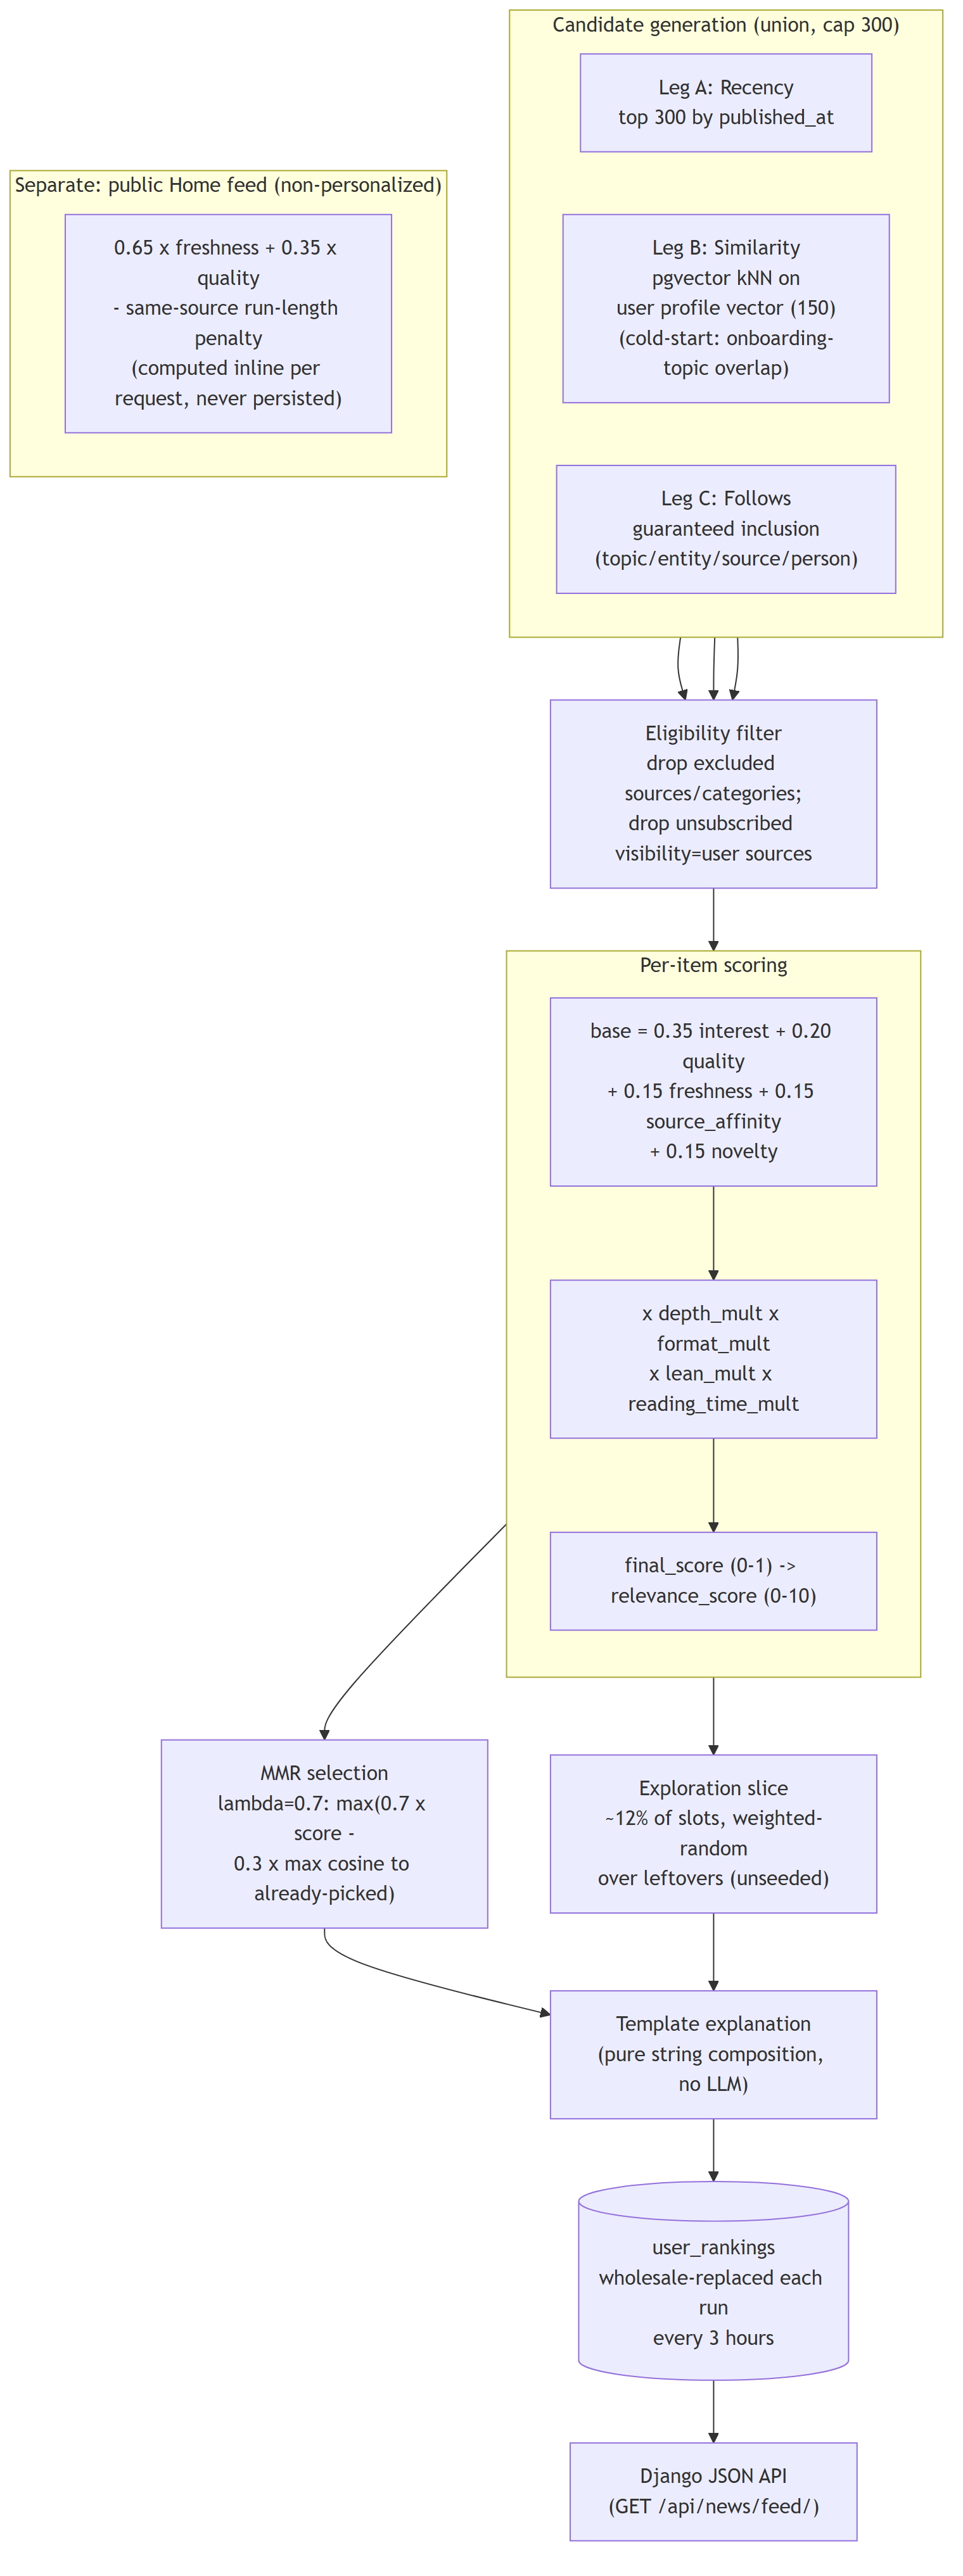
\includegraphics[width=0.55\textwidth,height=0.88\textheight,keepaspectratio]{figures/ranking_pipeline.png}
\caption{The personalized ranking pipeline: three-leg candidate generation, eligibility filtering, weighted-signal scoring, MMR diversification with a reserved exploration slice, and templated explanation generation.}
\label{fig:ranking-pipeline}
\end{figure}

Figure~\ref{fig:ranking-pipeline} lays out the personalized pipeline end to end. A feed request first applies the eligibility filter (Section~\ref{sec:rec-candidates}), then the surviving pool feeds the three-leg candidate union capped at 300 (Algorithm~\ref{alg:candidates}). Every candidate is scored deterministically through Equations~\ref{eq:ranking-base}--\ref{eq:ranking-relevance}, drawing on the nightly decayed affinities and profile vector (Equation~\ref{eq:affinity-decay}). Scored candidates pass through MMR selection (Equation~\ref{eq:mmr}), which fills most slots under the relevance/diversity trade-off, while a reserved exploration slice fills the remaining $\approx$12\% via a weighted random draw over MMR's leftovers. Every selected item, MMR-chosen or exploration-chosen, is paired with a templated explanation before persistence to \texttt{user\_rankings}. No stage calls a large language model.

Figure~\ref{fig:screenshot-myfeed} shows My Feed, the page this pipeline ultimately renders into for a signed-in user: each card is prefixed with the templated explanation string described in Section~\ref{sec:rec-explanations} (for example, ``Recommended because it published recently'' or ``Recommended because it from a source you engage with often, and published recently''), making the connection between the scoring pipeline and what the user actually sees directly visible rather than left to the reader's imagination.

\begin{figure}[htbp]
\centering
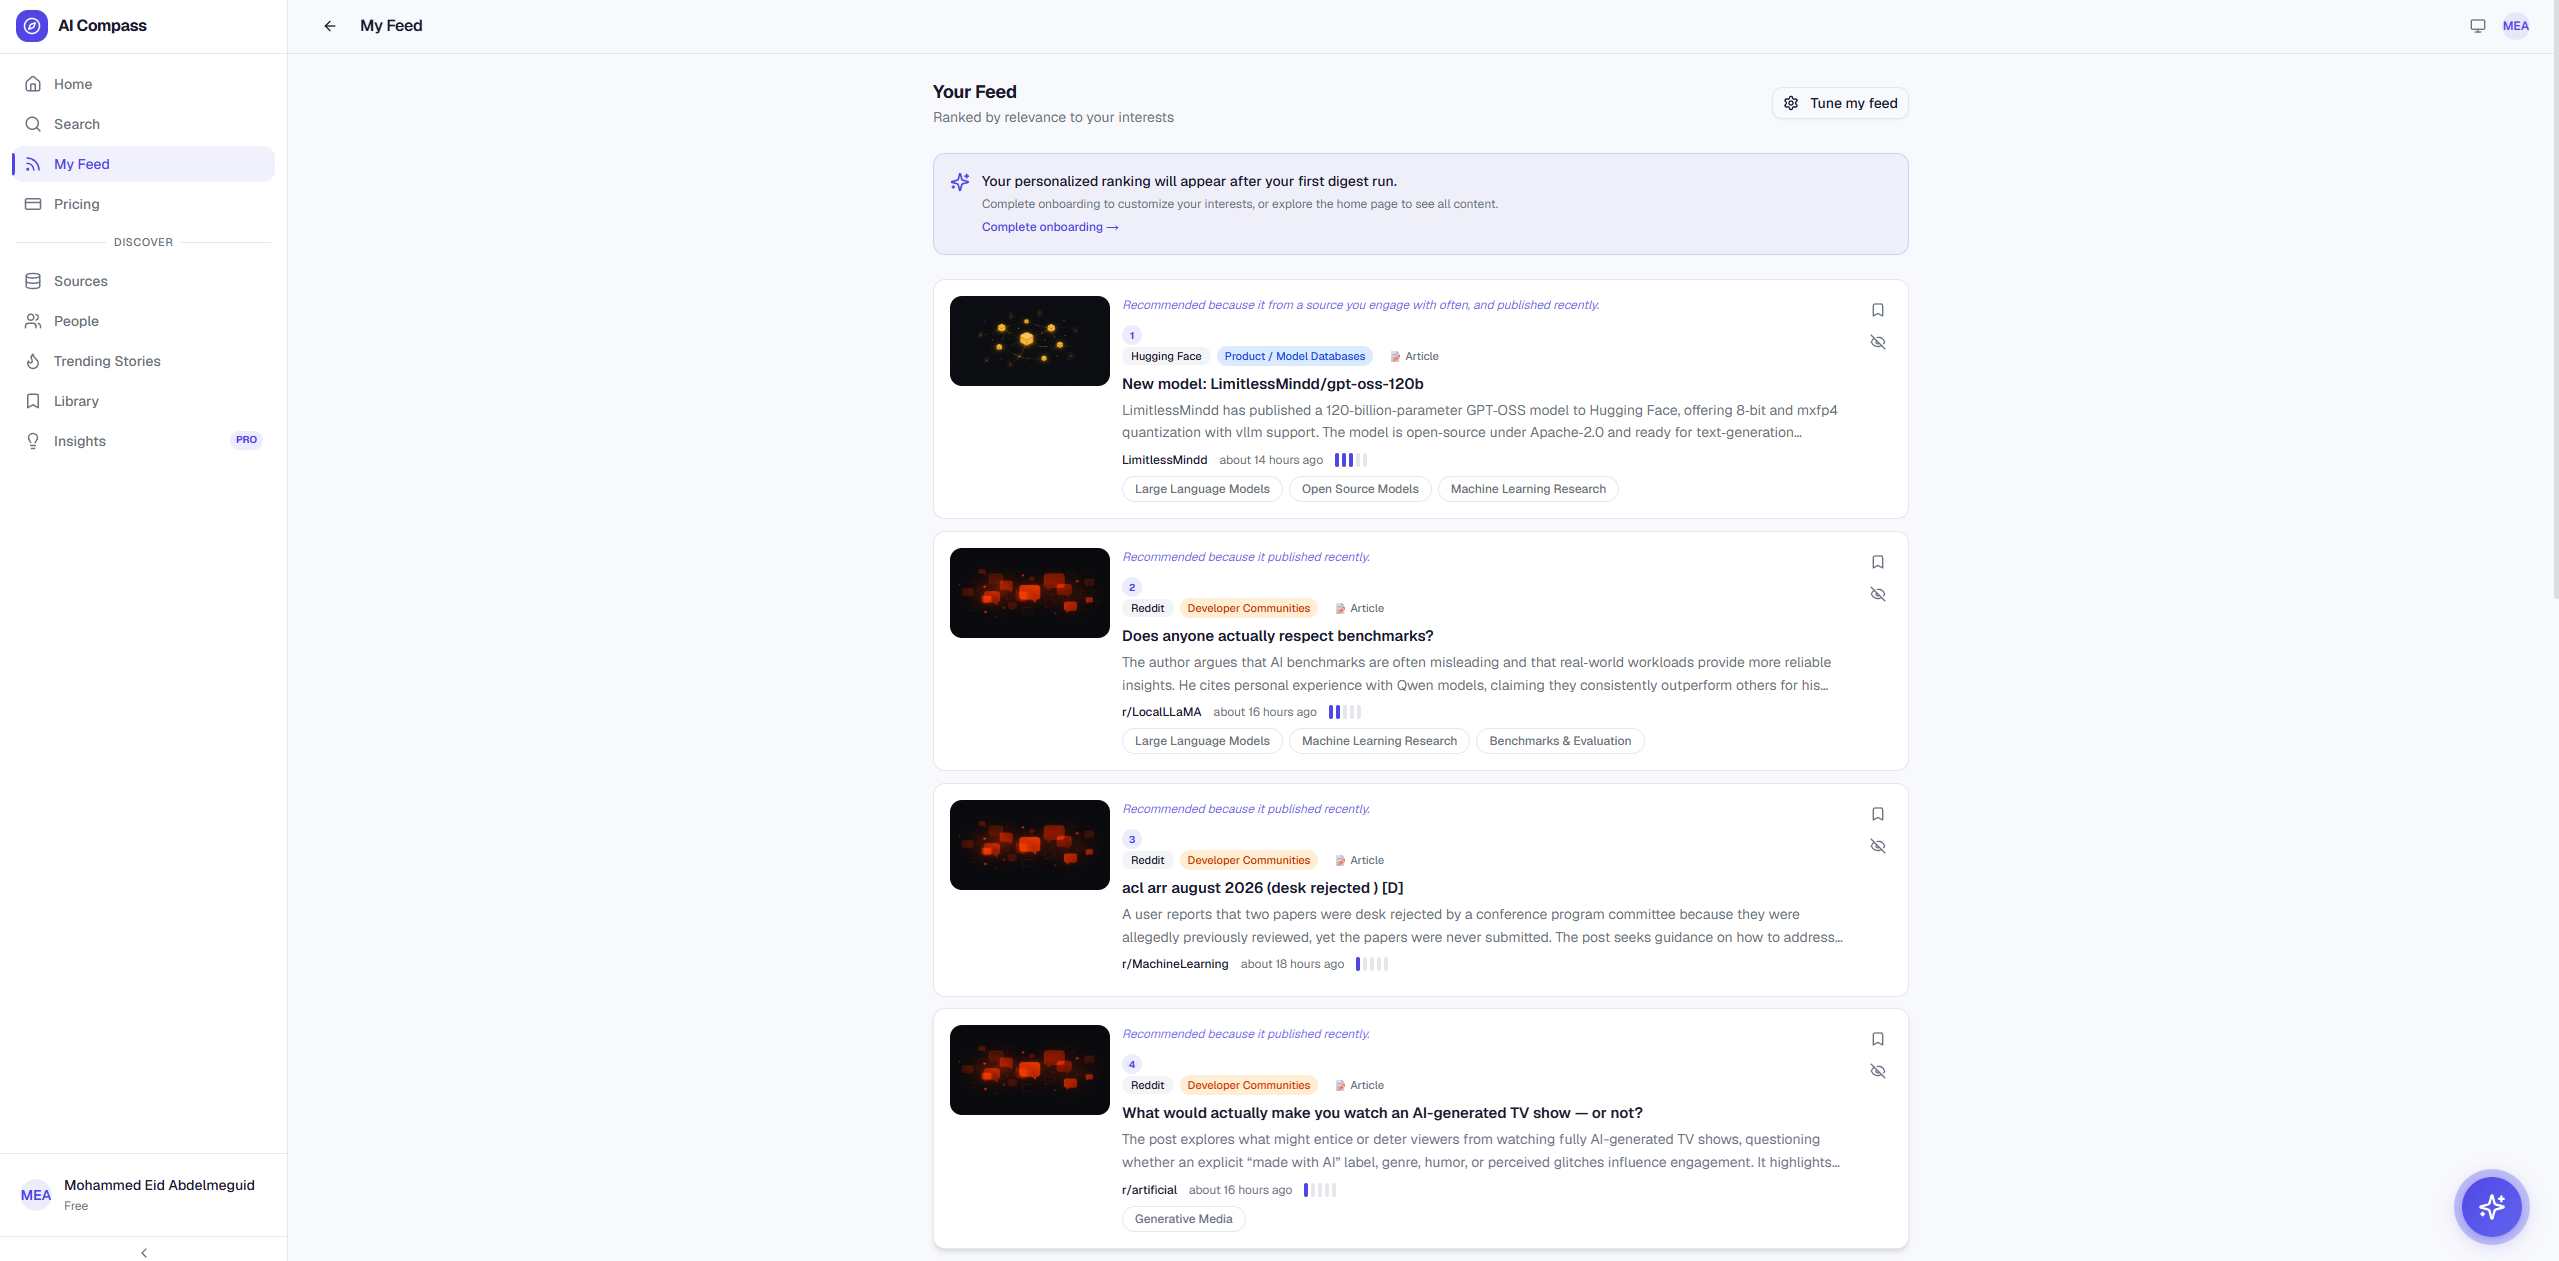
\includegraphics[width=0.85\textwidth]{figures/screenshots/screenshot_myfeed.png}
\caption{My Feed, showing the per-item templated explanation strings (Section~\ref{sec:rec-explanations}) that accompany each ranked recommendation.}
\label{fig:screenshot-myfeed}
\end{figure}

\section{Deliberately Deferred Approaches}
\label{sec:rec-deferred}

Several more sophisticated approaches were considered and explicitly left out of scope, rather than overlooked:

\begin{itemize}
  \item \textbf{Neural or learned ranking}: deferred; it would need substantially more logged interaction data than currently exists to train or validate, the same data-scarcity finding Chapter~10 documents directly.
  \item \textbf{Collaborative filtering}: deferred; the classic cold-start problem at a small user base leaves too little cross-user co-engagement signal to outperform the content-based approach already in place.
  \item \textbf{Per-persona summaries}: deferred to keep the one-LLM-call-per-item enrichment budget growing per-item, not per-user.
  \item \textbf{Region and language filters}: deferred; the current content pool and user base are not yet large or linguistically diverse enough for such filters to be meaningful.
  \item \textbf{Manual per-source weight sliders}: deferred in favor of the existing follow/exclude and source-affinity mechanisms, which already cover most of the same use case with less interface complexity.
  \item \textbf{Audience tags} (beyond the existing \texttt{technical\_depth} field): deferred as an enrichment dimension not yet justified by a concrete downstream use.
\end{itemize}

\section{Known Limitations of the Current Formula}
\label{sec:rec-limitations}

Three real, disclosed gaps are worth restating together, plainly, rather than left scattered.

First, \texttt{UserAffinity} maintains three dimensions (\texttt{topic}, \texttt{source}, \texttt{entity}), and entity-level affinity \emph{is} computed nightly (Section~\ref{sec:rec-signals}), but Equation~\ref{eq:ranking-base} only ever reads \texttt{topic} and \texttt{source} for $I$ and $S$; \texttt{entity} is computed but never consumed. This is a genuine, unaddressed gap, not a deliberate decision; the dimension exists specifically to feed personalization, and currently does not.

Second, the novelty signal $N$ (Section~\ref{sec:rec-score}) is tracked exclusively through digest-email click tokens, so it really measures ``not recently emailed,'' not ``not recently viewed on the web feed.'' A user who reads an item on the web but never receives it by email is scored as though it were fully novel indefinitely.

Third, the exploration slice's weighted draw (Section~\ref{sec:rec-mmr}) uses Python's unseeded \texttt{random.random()}, so exploration-slot items are not reproducible across repeated runs over an identical pool; the deterministic MMR-selected majority is unaffected, but the exploration slice cannot be replayed exactly without a seeded source.

None of these three gaps invalidate the ranker's core determinism claim for the MMR-selected portion of the list, and none were hidden in the implementation; all three are visible directly in the code and, in the case of the entity-affinity gap, in the mismatch between what is computed nightly and what the scoring function actually reads. They are recorded here, and again in Chapter~11, as concrete, well-scoped items for future work rather than as an indictment of the current design.

\chapter{Semantic Search and the RAG Conversational Assistant}
\label{chap:rag}

\section{Overview}
\label{sec:rag-overview}

The preceding chapters describe a serving path that is, by explicit architectural principle, deterministic and free of generative-model calls: the personalized feed (Chapter~\ref{ch:recommendation}) is produced by a fixed weighted formula, not by a language model reasoning about each candidate item. This chapter concerns the one part of AI Compass where that principle is deliberately relaxed: the conversational assistant, which exists because a ranked list of items, however well personalized, cannot answer a free-form question such as ``what does this mean?'' or ``which of these releases support long-context inference?''. The assistant is built on the retrieval-augmented generation (RAG) pattern: a \emph{retrieval} model, running over embeddings of the ingested corpus, selects a small set of passages relevant to the user's question, and a separate \emph{generation} model produces an answer conditioned only on those passages \cite{lewis2020rag}. Retrieval is embedding-based, deterministic given its inputs, and never calls a large language model; generation is the one step in the entire request-serving path that does. Conflating the two would misrepresent AI Compass as an application whose every request passes through a language model, when the ranking and browsing hot path (Chapter~\ref{ch:recommendation}) deliberately does not. The rest of this chapter follows the pipeline in order: chunking and indexing, retrieval and access control, generation and grounding checks, multi-turn conversation, and streaming.

Figure~\ref{fig:screenshot-search} shows the platform's search surface, which is the semantic/keyword search feature referenced above rather than the conversational assistant itself: a query for ``llm quantization techniques'' returning real, currently-indexed arXiv and Reddit results on quantization methods, each carrying its source, category, and topic tags. The assistant itself is a separate, chat-style panel, shown open alongside an article in Figure~\ref{fig:screenshot-rag-chat}.

\begin{figure}[htbp]
\centering
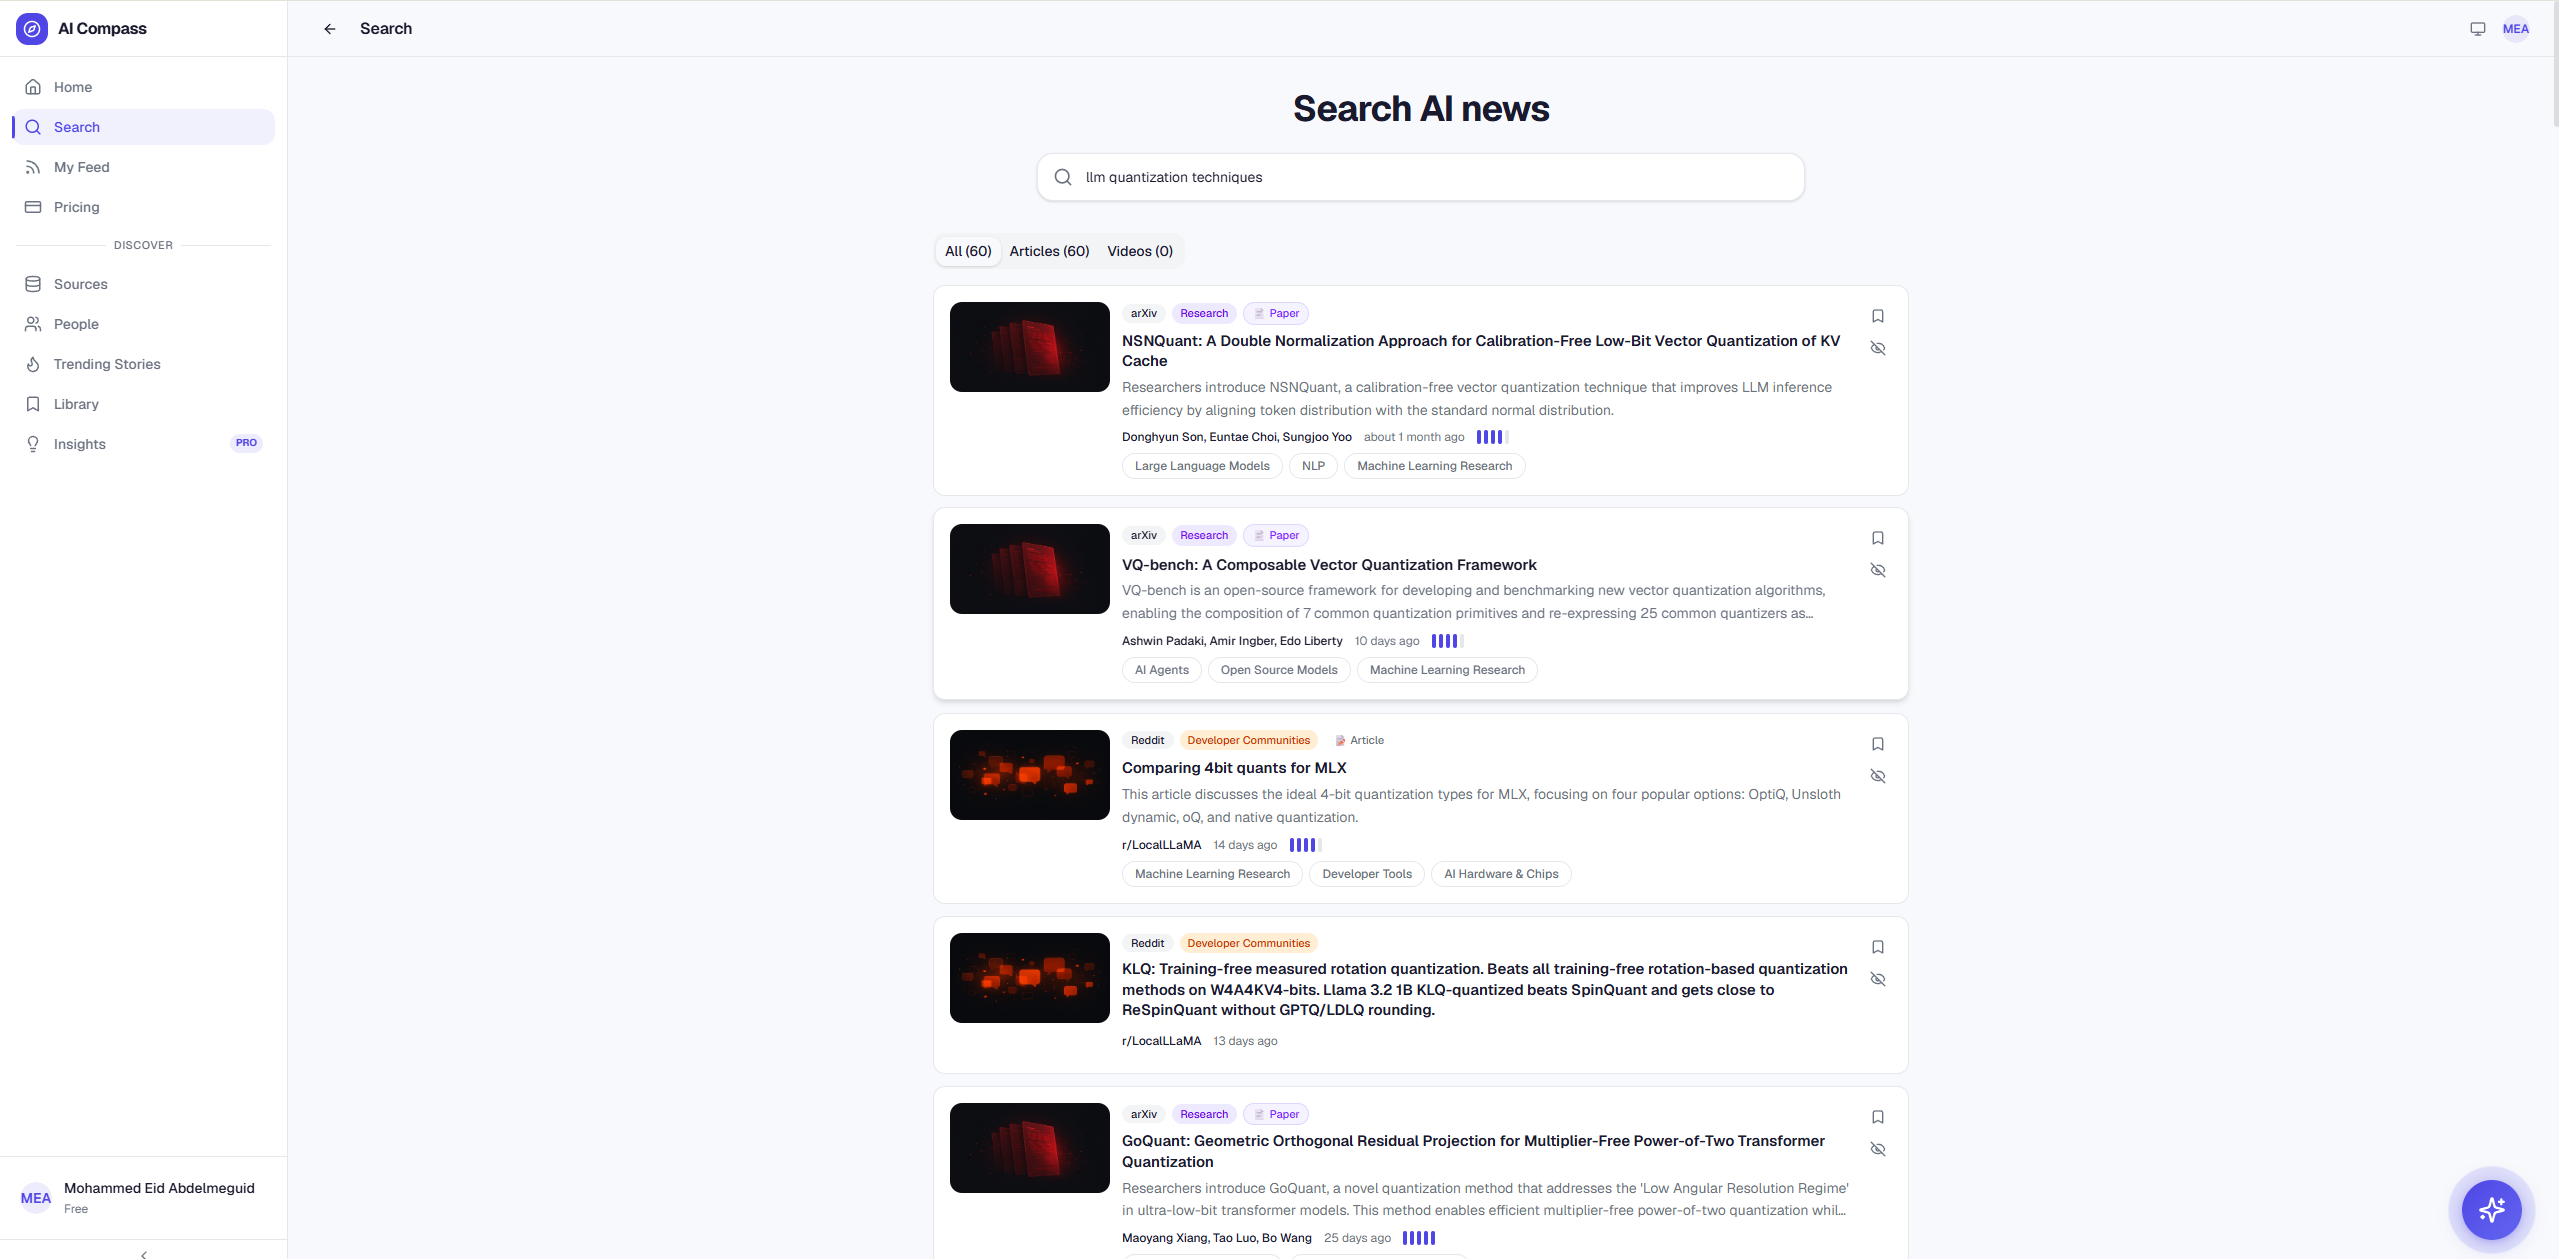
\includegraphics[width=0.85\textwidth]{figures/screenshots/screenshot_search.png}
\caption{The AI Compass search surface, showing results for the query ``llm quantization techniques.''}
\label{fig:screenshot-search}
\end{figure}

\begin{figure}[htbp]
\centering
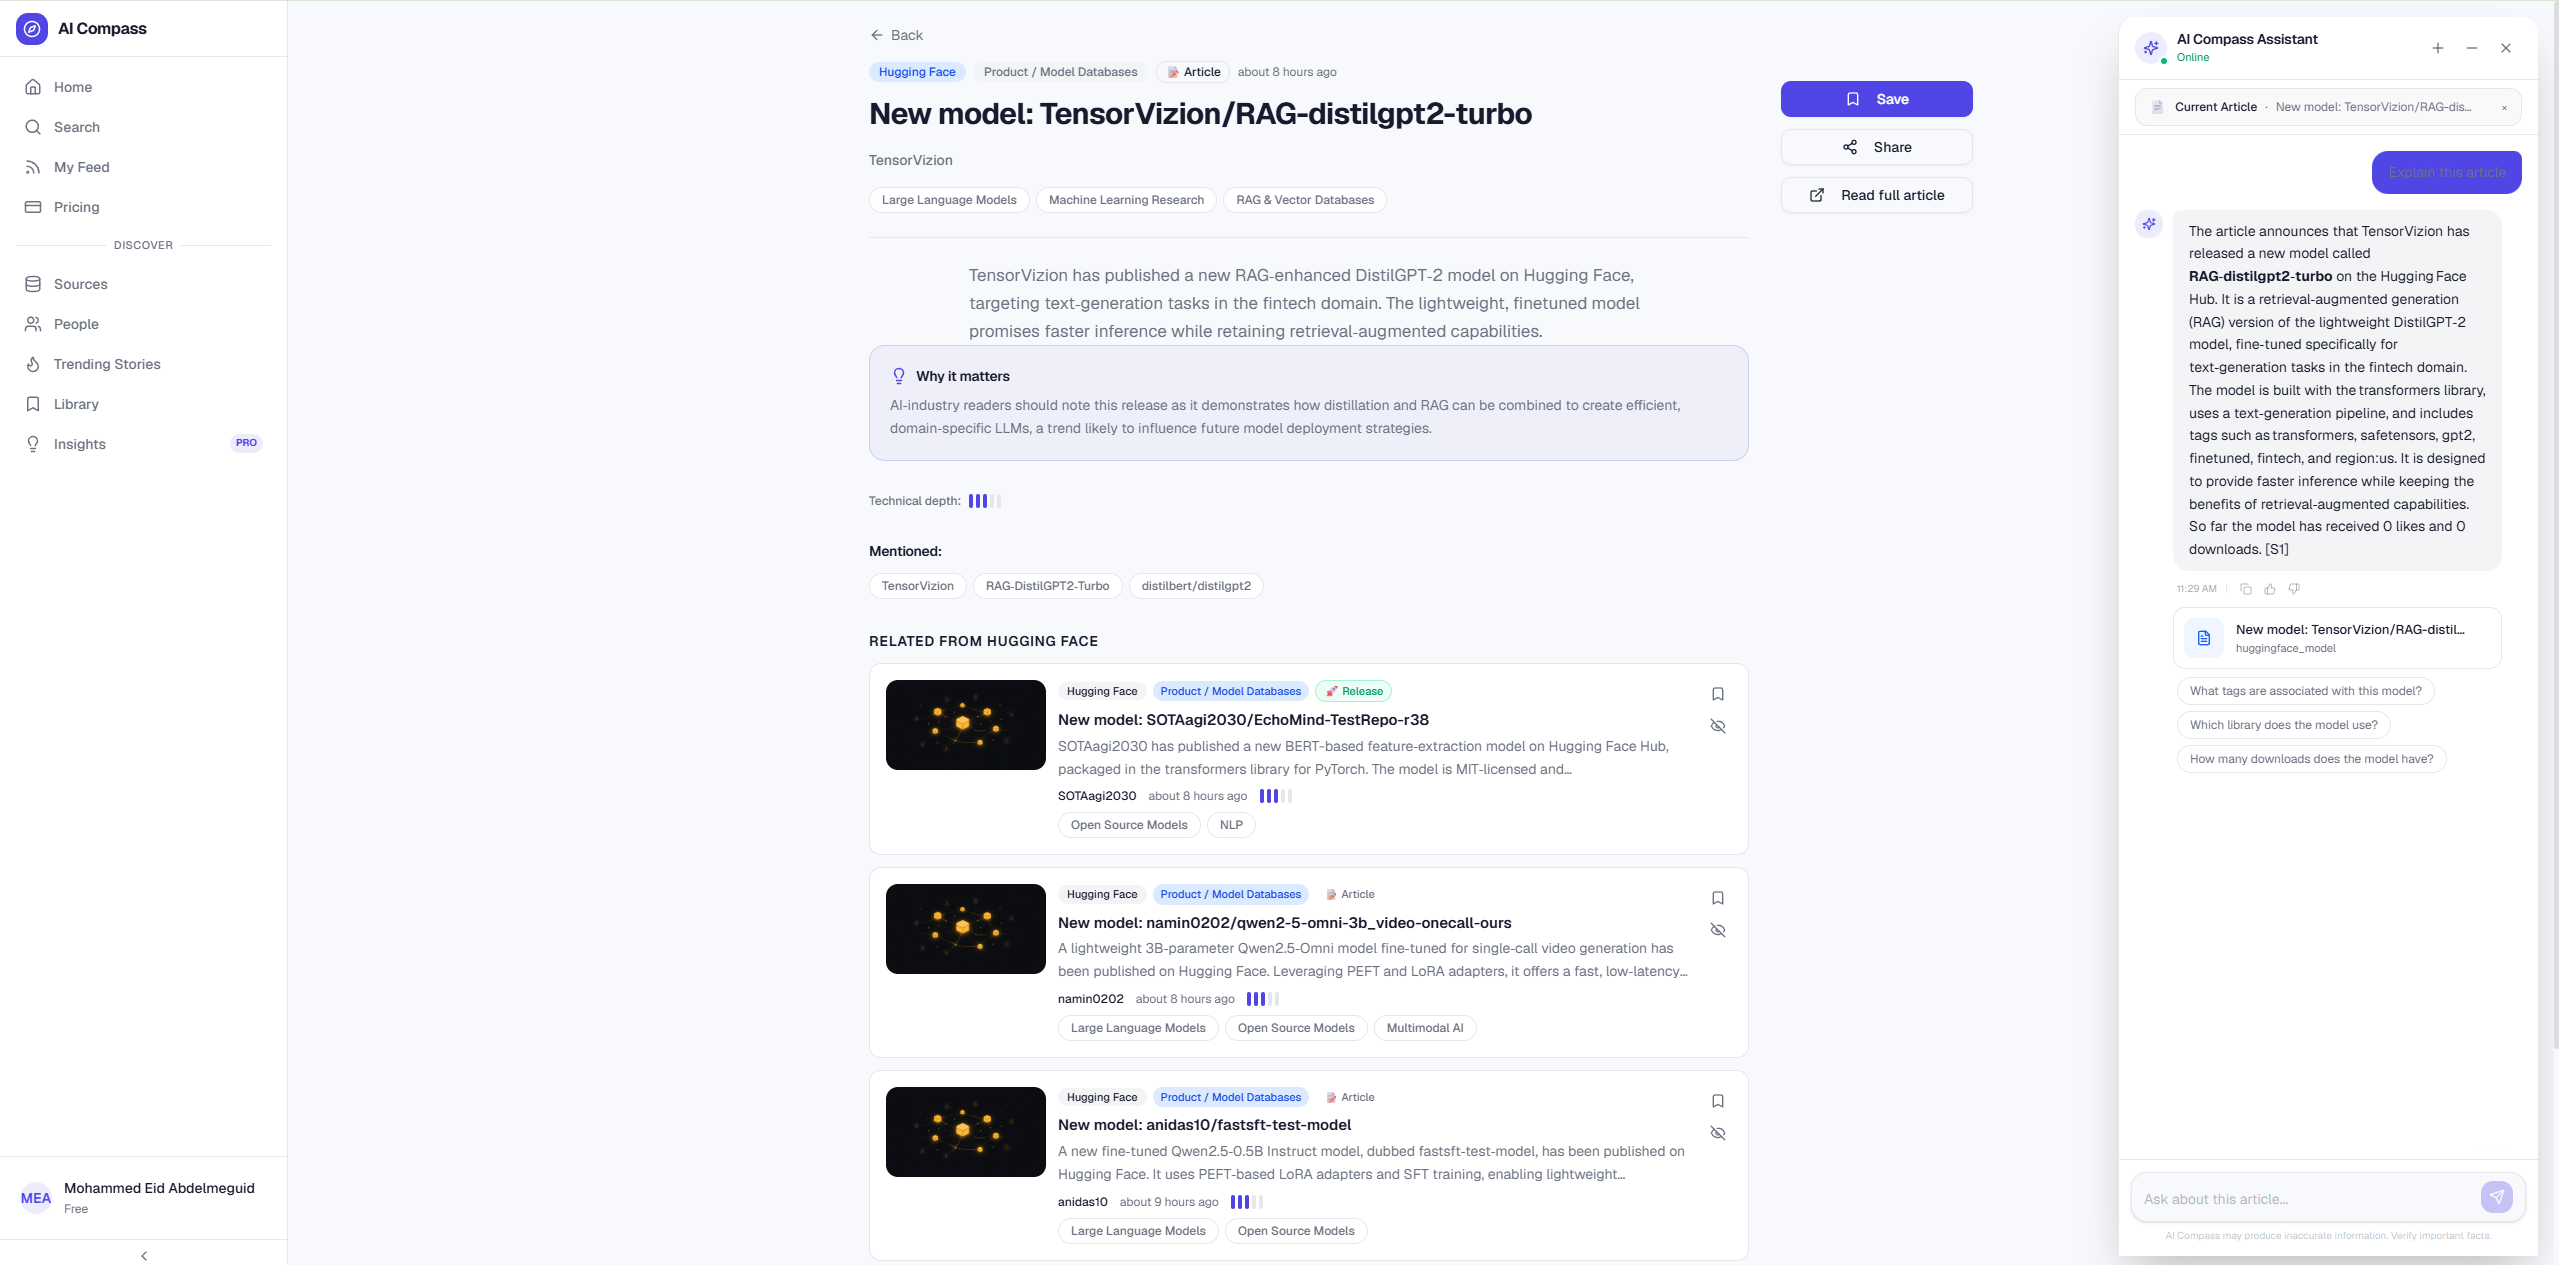
\includegraphics[width=0.85\textwidth]{figures/screenshots/screenshot_article_chat.png}
\caption{The RAG conversational assistant open alongside an article, with a numbered \texttt{[S\#]} citation resolved to a source card and follow-up suggestion chips generated by the same call (Section~\ref{sec:rag-multiturn}).}
\label{fig:screenshot-rag-chat}
\end{figure}

\section{Passage Chunking}
\label{sec:rag-chunking}

Retrieval-augmented generation operates over passages, not whole documents: a long document must be cut into smaller units before it can be embedded and searched at passage granularity, since embedding an entire document into one vector discards exactly the fine-grained detail a specific question is likely to ask about. AI Compass implements two chunkers feeding the same downstream embedding step. A sentence-based chunker is used for prose (articles): it accumulates whole sentences into a passage and carries the passage's starting and ending character offsets, later letting a citation link back to a specific span of the original text. A segment-based chunker is used for video transcripts: it accumulates transcript segments, each already carrying a start/end timestamp from the captioning or speech-to-text stage (Chapter~\ref{chap:deep-media}), and propagates those timestamps onto the resulting passage so a citation into a video can deep-link to the exact playback position (a \texttt{?t=} parameter) rather than only naming the video.

Both chunkers share the same size budget: a target passage length of $\approx$180 tokens, an overlap of $\approx$40 tokens between consecutive passages so a fact spanning a boundary is not orphaned in exactly one chunk, and a hard cap of 240 tokens. This budget exists for a concrete reason: the embedding model used throughout AI Compass, \texttt{all-MiniLM-L6-v2} (Chapter~\ref{ch:background}), silently truncates any input beyond 256 word-piece tokens rather than raising an error, so a passage embedded past that ceiling would have its tail silently discarded with no signal anything was lost. Targeting $\approx$180 with a 240 hard cap leaves a working margin under the model's true 256-token ceiling.

The project uses no real subword tokenizer (no \texttt{tiktoken} dependency); token counts are instead estimated from word counts via $\hat{n}_{\text{tok}} \approx n_{\text{words}} / 0.75$ (Equation~\ref{eq:token-heuristic}), reflecting the rough English-language rate of $\approx$1.33 word-piece tokens per word, an honest approximation, not an exact count, and stated as such here. The design does not rely on the heuristic alone for correctness: the embedding model's own 256-token truncation is the real backstop, so an under- or over-estimate produces at worst a passage a little shorter or longer than the $\approx$180-token target, never one that silently loses content, since the 240-token hard cap already sits below the model's actual ceiling.

\begin{equation}
  \hat{n}_{\text{tok}} \approx \frac{n_{\text{words}}}{0.75}
  \label{eq:token-heuristic}
\end{equation}

\section{Passage Indexing}
\label{sec:rag-indexing}

Once chunked, every passage is embedded with the same \texttt{all-MiniLM-L6-v2} model already used elsewhere in the platform (384-dimensional, run locally rather than through a hosted embedding API), and the resulting vectors are stored in a table dedicated to this purpose, \texttt{rag\_chunks}, rather than in the general-purpose \texttt{embeddings} table that the ranking and clustering subsystems already use for one-embedding-per-item vectors.

This separation is a deliberate architectural decision, not an oversight. The existing \texttt{embeddings} table is read by two other subsystems (near-duplicate clustering, Chapter~\ref{ch:data-pipeline}; ranking candidate generation, Chapter~\ref{ch:recommendation}) under an implicit but load-bearing assumption: exactly one embedding per content item. A passage-level chunk breaks that assumption outright: a single long article can produce a dozen or more chunk embeddings. Writing chunk vectors into the shared table would have silently pulled passage rows into clustering and profile-vector searches as if they were independent items, a subtle bug that would surface only as slow quality degradation, not an error. A dedicated table sidesteps this entirely: neither existing caller needs to change, or even be aware, that passage-level chunking exists.

The \texttt{rag\_chunks} table carries a pgvector index built on the Hierarchical Navigable Small World (HNSW) graph structure, using cosine distance as its similarity metric,
\begin{equation}
  d_{\cos}(\mathbf{q}, \mathbf{c}) = 1 - \frac{\mathbf{q} \cdot \mathbf{c}}{\lVert \mathbf{q} \rVert \, \lVert \mathbf{c} \rVert},
  \label{eq:cosine-distance}
\end{equation}
computed between a query embedding $\mathbf{q}$ and a candidate chunk embedding $\mathbf{c}$, with nearer neighbors (those with the smallest $d_{\cos}$) approximated by traversing the HNSW graph rather than by an exhaustive scan of every stored vector. This is the first approximate-nearest-neighbor index anywhere in the project: the pre-existing \texttt{embeddings} table, by contrast, has no ANN index of any kind, so a nearest-neighbor query against it falls back to an exact, exhaustive comparison, a limitation unrelated to the RAG assistant itself, but worth noting here because it means the retrieval path described in the rest of this chapter is, at the time of writing, the only part of AI Compass whose vector search is backed by genuinely sub-linear approximate search rather than a full scan.

\section{Retrieval}
\label{sec:rag-retrieval}

A question is first routed to one of three retrieval scopes: \emph{document} scope, when asked from a specific article or video detail page (the canonical case being ``what does this mean?'', which carries no subject of its own and must be interpreted against the page currently viewed); \emph{topic} scope, anchored to a topic rather than a single item; or an unscoped general knowledge-base query. The chosen scope can augment the query text before embedding (e.g. folding in the current page's title), and can change mid-conversation, since scope is recorded per message rather than locked to the conversation.

Once the (possibly scope-augmented) query is embedded, retrieval deliberately over-fetches $k' = \text{top\_k} \times 6$ (Equation~\ref{eq:overfetch}) candidates from the HNSW cosine search, where $\text{top\_k}$ defaults to 8, giving $k'=48$ candidates pulled back before any filtering. Over-fetching exists because the next stage (an access-control filter, Section~\ref{sec:rag-access-control}) removes an a priori unknown fraction of the result, and fetching only the final target count would risk too few, or zero, surviving passages whenever a meaningful share of the nearest neighbors belong to sources the requester cannot see.

\begin{equation}
  k' = \text{top\_k} \times 6
  \label{eq:overfetch}
\end{equation}

Surviving candidates then pass into a greedy selection step bounded by two constraints at once: a 2200-token total context budget, and a per-document diversity cap of at most 3 chunks, so one long, highly relevant document with many overlapping high-similarity chunks cannot crowd out every other relevant source.

Finally, if the filtering and selection steps leave nothing to answer with, the system does not simply return an empty context. Section~\ref{sec:rag-fallback} below describes the deterministic, non-vector fallback that recovers from exactly this case using the page the user is currently viewing, when one exists. Algorithm~\ref{alg:rag-retrieval} summarizes the full retrieval pipeline described in this section, from query embedding through to that fallback.

\begin{algorithm}[htbp]
  \small
  \DontPrintSemicolon
  \KwInput{query $q$, scope $s$, requesting user $u$, current-page document $d_{\text{page}}$ (may be null), $\text{top\_k}$ (default 8), token budget $B$ (2200), per-document cap $c$ (3)}
  \KwOutput{an ordered list of source passages $\mathcal{S}$, each carrying a citation number}
  $q' \leftarrow \textsc{AugmentByScope}(q, s)$\;
  $\mathbf{v} \leftarrow \textsc{Embed}(q')$ \tcp*{same model used to index \texttt{rag\_chunks}}
  $C \leftarrow \textsc{HNSWCosineSearch}(\mathbf{v}, k = \text{top\_k} \times 6)$ \tcp*{over-fetch, up to 48 candidates}
  $C \leftarrow \{\, c \in C : \textsc{PassesAccessControl}(c, u) \,\}$ \tcp*{Section~\ref{sec:rag-access-control}}
  sort $C$ by descending similarity to $\mathbf{v}$\;
  $\mathcal{S} \leftarrow \emptyset$; $\text{tokens\_used} \leftarrow 0$; $\text{count}[\cdot] \leftarrow 0$\;
  \ForEach{$c \in C$}{
    \If{$\text{tokens\_used} + |c| \le B$ \textbf{and} $\text{count}[\text{doc}(c)] < c_{\text{cap}}$}{
      $\mathcal{S} \leftarrow \mathcal{S} \cup \{c\}$\;
      $\text{tokens\_used} \leftarrow \text{tokens\_used} + |c|$\;
      $\text{count}[\text{doc}(c)] \leftarrow \text{count}[\text{doc}(c)] + 1$\;
    }
  }
  \If{$\mathcal{S} = \emptyset$ \textbf{and} $d_{\text{page}} \ne \text{null}$ \textbf{and} \textsc{PassesAccessControl}($d_{\text{page}}$, $u$)}{
    $\mathcal{S} \leftarrow \{\, \textsc{RawContent}(d_{\text{page}})[\,:9000\,] \,\}$ \tcp*{deterministic fallback, Section~\ref{sec:rag-fallback}}
  }
  \Return{\textsc{Numbered}($\mathcal{S}$)}
  \caption{RAG passage retrieval}
  \label{alg:rag-retrieval}
\end{algorithm}

\section{Access Control and Private Sources}
\label{sec:rag-access-control}

AI Compass lets users exclude entire sources or categories from their own feed, and subscribe to sources with restricted visibility, including ones they submitted themselves. Because retrieval draws candidates from the same shared \texttt{rag\_chunks} index for every user, nothing about the HNSW similarity search itself prevents a query from surfacing a passage the requester should never see; the access-control filter closes that gap and is a genuine, disclosed leak-prevention mechanism, not an incidental feature.

The filter applies two independent conditions to every candidate chunk. First, a chunk is dropped if its source is among the requesting user's excluded sources or categories: the same exclusion mechanism governing the personalized feed is honored here. Second, a chunk is dropped if its source is marked \texttt{visibility='user'} (submitted for private use, not curated public content) and the requester is not a subscriber, the more security-relevant condition, since without it one user's private source material could be retrieved and quoted to an unrelated user simply for being the closest semantic match.

Critically, this same filter also applies to the current-page document consulted by the deterministic fallback below: a private, unsubscribed document cannot become answerable material merely because a user is viewing its detail page.

\section{Answer Generation and Anti-Hallucination Mechanisms}
\label{sec:rag-generation}

Once a set of numbered source passages has been assembled, generation is performed by Groq's hosted \texttt{llama-3.3-70b-versatile} model, with \texttt{max\_tokens} bounded at 700 and temperature set to 0.3. The 700-token bound is the first hard \texttt{max\_tokens} limit anywhere in this codebase, a deliberate cost- and latency-control decision: an unbounded call on the project's largest model tier would expose per-message cost and latency to whatever length the model chose, rather than to an operator-capped length. The moderate, non-zero temperature (versus temperature-0 for the smaller condensation model, Section~\ref{sec:rag-multiturn}) reflects that answer generation is a synthesis task where some lexical variety is desirable, unlike condensation, which should be as deterministic as possible.

Three anti-hallucination mechanisms work together. First, the system prompt requires every substantive claim to carry a numbered \texttt{[S\#]} marker matching a supplied source, and instructs the model never to invent one, necessarily advisory, since nothing prevents a model from disregarding an instruction. Second, and server-side: every \texttt{[S\#]} marker in the returned answer is checked by regular expression against the genuinely supplied source numbers, and any marker that fails to resolve is surgically removed inline, rather than triggering a whole-sentence or whole-answer rejection; natural-language prose does not decompose into independently droppable units the way a bulleted list does, so discarding an entire sentence or answer around one bad marker would throw away legitimate cited content along with it. Third, a \texttt{grounded} boolean is set to \texttt{false} only when \emph{every} marker in the raw answer failed to resolve (the model appears to have ignored the sources entirely), remaining \texttt{true} if at least one marker resolved even when others did not, a threshold chosen so one slipped citation number does not flag an otherwise well-supported answer as ungrounded, while the all-fail case remains a strong, actionable signal.

\section{Multi-Turn Conversation}
\label{sec:rag-multiturn}

A conversational assistant must resolve a follow-up such as ``can you simplify that?'' into something retrieval can act on, since neither the phrase nor its embedding carries any information about what ``that'' refers to. AI Compass addresses this with a query-condensation step running before retrieval on every turn after the first: given the last 6 messages of history, a separate, cheaper (8B-class) Groq model at temperature 0 rewrites the follow-up into a standalone question. The rewritten question, not the literal follow-up text, is what gets embedded and retrieved against.

Because this call sits on the critical path of every follow-up turn, its failure mode is conservative: any failure falls back to the raw original question rather than blocking the turn, so a follow-up degrades gracefully to ``retrieval against the literal text'' instead of failing outright. Stored conversation history is capped server-side at 8 messages ($\approx$4 turn pairs), bounding both the condensation prompt and retained state.

A closely related feature costs nothing extra: the same generation call (Section~\ref{sec:rag-generation}) is instructed to append a trailer line \texttt{SUGGESTIONS: q1 | q2 | q3}, parsed out server-side by regex and never shown raw. Since suggestions come from the same call that produces the answer, this costs zero additional model round-trips, a feature that otherwise could have doubled per-message cost as a second, dedicated call.

\section{Streaming Architecture}
\label{sec:rag-streaming}

AI Compass exposes the assistant over two HTTP mechanisms: a conventional, non-streaming JSON endpoint returning a complete answer in one response, and a server-sent-events (SSE) endpoint streaming the answer token by token. These two paths are not deployed identically. The bulk of the Django backend (including the non-streaming chat endpoint and every other view) runs under gunicorn as a standard synchronous WSGI service with a small, fixed worker pool. Only the streaming SSE endpoint runs on a second, dedicated ASGI process (uvicorn), in its own container. It would be equally imprecise to call the backend uniformly WSGI or uniformly ASGI; the accurate statement is that the bulk of it is WSGI, and only the streaming chat path is carved out onto an isolated ASGI process.

The reason follows directly from what a long-lived streaming connection does to a small, fixed worker pool: a synchronous WSGI worker is occupied for a request's entire duration, so serving a token-by-token stream from a main-service gunicorn worker would tie it up, unavailable to any other request, for as long as the connection stayed open. Isolating the streaming endpoint means a slow or long-lived chat stream can never starve the main service's worker pool.

This split is also the one deliberate, disclosed exception to a broader principle holding everywhere else in the project: the Django web tier makes no direct LLM calls of its own, and every other LLM call happens inside the pipeline's Celery worker processes, not inside a Django request. The streaming endpoint is the exception because it needs its own lightweight Groq client living directly in Django: a Celery task boundary suits a bounded unit of work that reports back once finished, but has no mechanism for streaming individual tokens back to an already-open HTTP connection, which is exactly what SSE requires.

\section{Pipeline Summary}
\label{sec:rag-summary}

\begin{figure}[htbp]
  \centering
  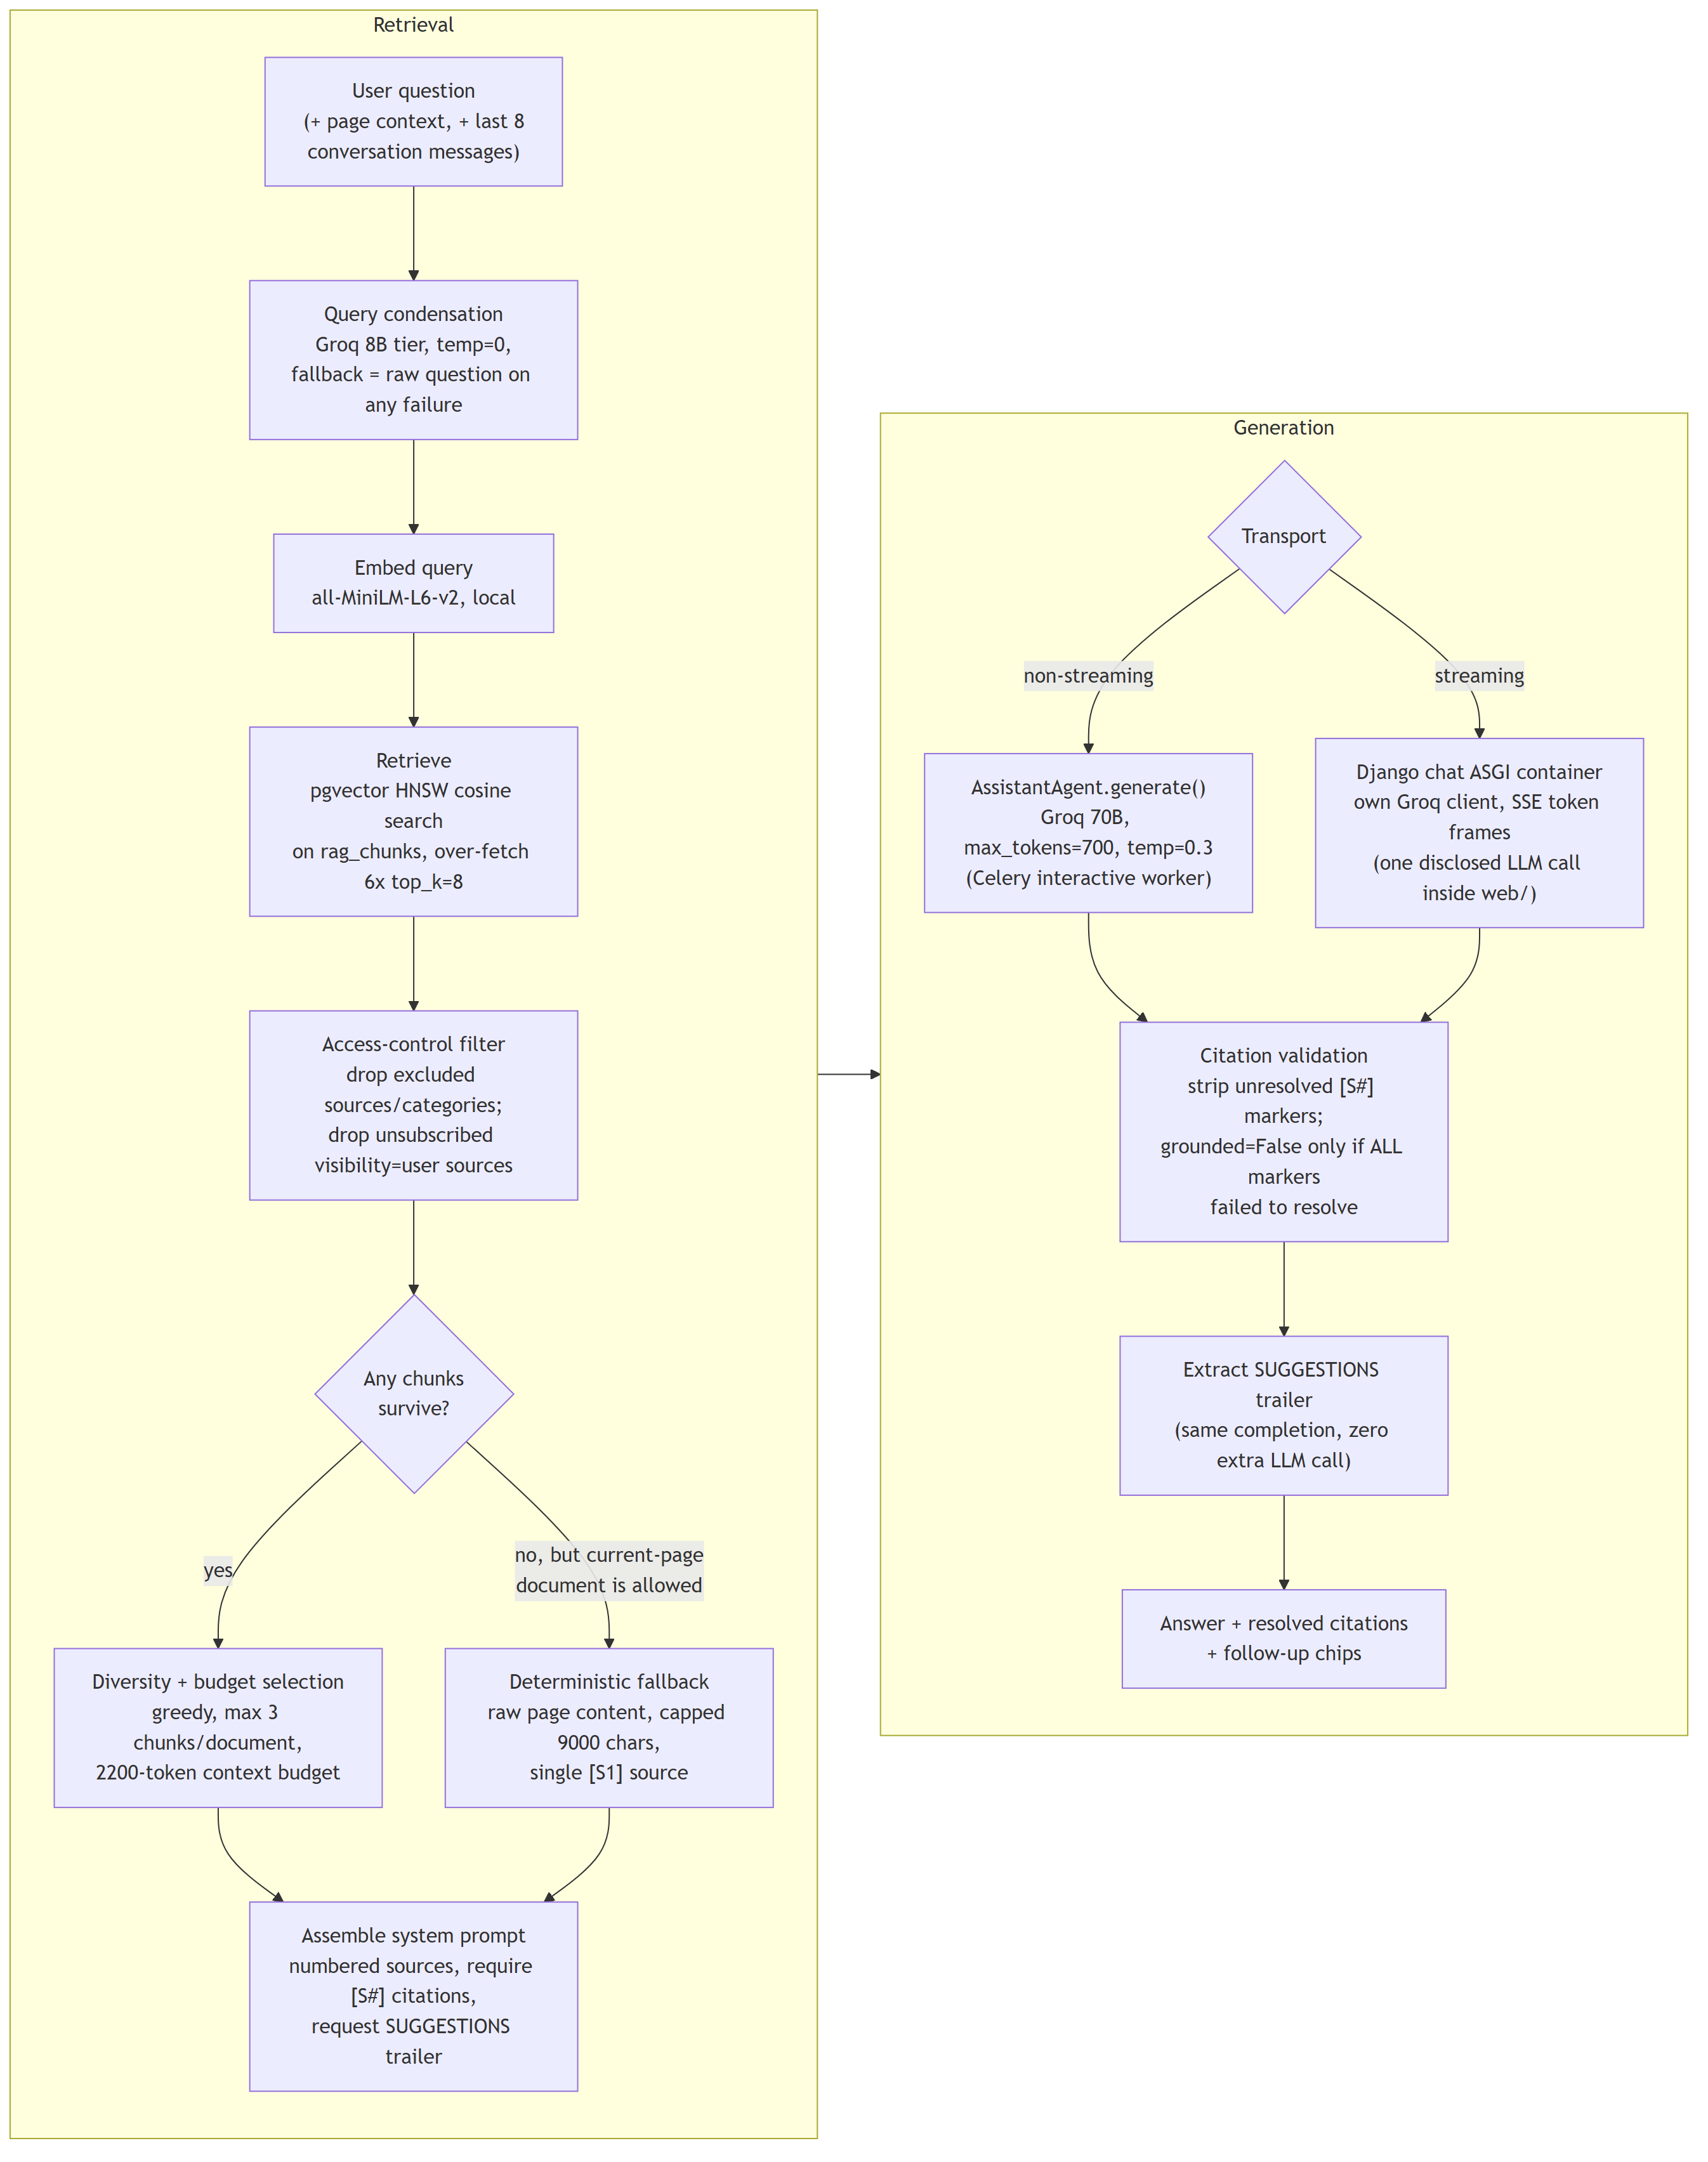
\includegraphics[width=0.85\textwidth,height=0.85\textheight,keepaspectratio]{figures/rag_pipeline.png}
  \caption{The RAG assistant's retrieval and generation pipeline, from query condensation through access-controlled retrieval to citation-validated generation.}
  \label{fig:rag-pipeline}
\end{figure}

Figure~\ref{fig:rag-pipeline} traces the full path a message takes through the assistant, drawing together every mechanism described in this chapter. A follow-up message is first condensed, with a raw-question fallback, into a standalone query (Section~\ref{sec:rag-multiturn}). The query is routed to a retrieval scope and embedded with the same model used to index passages (Section~\ref{sec:rag-retrieval}), then matched against the \texttt{rag\_chunks} HNSW cosine index with a $6\times$ over-fetch. The access-control filter removes any passage the requesting user is not entitled to see, whether by exclusion or by unsubscribed private-source visibility (Section~\ref{sec:rag-access-control}), before a greedy, budget- and diversity-capped selection assembles the final numbered source list, falling back to the current page's raw content when nothing else survives (Section~\ref{sec:rag-fallback}, folded into Algorithm~\ref{alg:rag-retrieval}). Generation then produces a citation-bearing answer and an appended suggestions trailer in a single model call, after which server-side regex validation strips unresolvable citation markers and sets the \texttt{grounded} flag (Section~\ref{sec:rag-generation}). Finally, the answer is either returned as one JSON payload or streamed token by token from the isolated ASGI process described in Section~\ref{sec:rag-streaming}, depending on which endpoint the frontend called.

\subsection{Deterministic Fallback for Freshly Indexed Content}
\label{sec:rag-fallback}

One consequence of the pipeline above is worth stating on its own, since it explains a behavior a user is likely to notice directly. If the greedy selection step in Algorithm~\ref{alg:rag-retrieval} produces an empty passage set (most commonly because a page was indexed too recently for its chunks to have propagated, or because no chunk scored highly enough to survive filtering), the system checks whether the current page's own document passes the same access-control filter described in Section~\ref{sec:rag-access-control}. If it does, that document's raw content, truncated to the first 9000 characters, is used directly as the sole numbered source for the answer, bypassing vector search entirely. This deterministic, non-vector fallback is why a question such as ``summarize this article,'' asked from an article's own detail page, reliably works even on a page freshly indexed with no other passages yet found similar to the question; the fallback does not depend on the passage index having caught up at all.

\section{Limitations}
\label{sec:rag-limitations}

Two limitations of the RAG subsystem are worth stating plainly rather than glossed over. First, no automated test coverage was found for the RAG service or its retrieval logic; this was confirmed by a repository-wide search for test files, which turned up none exercising the chunking, retrieval, access-control, or generation code paths described in this chapter. Every behavior described here has been verified by direct code reading and by manual, live, browser-driven verification sessions rather than by an automated test suite, and the absence of that suite should be read as a genuine gap rather than an implicit claim of tested correctness.

Second, the deterministic fallback described in Section~\ref{sec:rag-fallback} is itself only a partial remedy for a freshly indexed or otherwise poorly matched document. Its 9000-character cap means that a document substantially longer than that is only partially visible to the assistant even while the fallback is active: the model is given the first 9000 characters of the page's raw content, not the whole document, so a question whose answer depends on material past that cutoff can go unanswered by the fallback in exactly the same way it could by an incomplete vector-search result. The fallback closes the specific gap of ``nothing was retrieved at all''; it does not, by itself, guarantee that the entirety of a long document is available to the model.

\chapter{Deep Media Processing}
\label{chap:deep-media}

Long-form video is structurally unlike every other source type AI Compass ingests: a research preprint or a government notice arrives as text the enrichment agent can read directly, but a video's substantive content is locked inside an audio track until something turns it into text. This chapter documents how the pipeline acquires a transcript for every ingested YouTube video, how it falls back to local speech-to-text when no caption track exists, how it copes with videos long enough that a single enrichment pass over the full transcript is neither practical nor within the system's own truncation limit, and how the resulting per-chapter summaries are exposed differently to Free and Pro viewers without duplicating the underlying computation.

\section{Caption Retrieval and STT Fallback}
\label{sec:deep-media-captions}

Every scraped YouTube video first attempts a caption-based transcript rather than committing directly to transcription. The caption-fetch step tries three sources in a fixed priority order: a manually created English caption track, if the uploader supplied one; failing that, an auto-generated English caption track; and failing that, an auto-generated caption track in any other language, machine-translated to English. This ordering reflects a simple accuracy hierarchy (a human-authored caption is trusted over a machine-generated one in the same language, which is in turn trusted over a machine-generated caption that has passed through an additional translation step), and it means the majority of videos that any caption track at all, in any language, never need to reach the transcription stage described in Section~\ref{sec:deep-media-transcription}.

When none of the three caption sources yields anything, the video is not dropped or deferred: it is still inserted into the corpus, with its content field left empty, and a speech-to-text job is queued against it in a dedicated \texttt{stt\_jobs} table with status \texttt{queued}. Keeping the video row in place rather than withholding it until a transcript exists means the item can already participate in title-only discovery and does not silently vanish from the pipeline's bookkeeping while transcription is pending.

An STT job moves through five possible states over its lifetime: \texttt{queued}, \texttt{running}, \texttt{completed}, \texttt{failed}, and \texttt{skipped\_too\_long} (the last of these is produced by the duration gate described in Section~\ref{sec:deep-media-transcription}, not by a transcription failure). The dispatch phase that hands queued jobs off to a Celery worker is written specifically to avoid a race between the database and the task queue: it claims a batch of queued jobs by flipping their status to \texttt{running} and \emph{committing that state change} before it calls the worker task that will actually perform the transcription. This ordering is deliberate rather than incidental: if the dispatch phase instead queued the worker task first and updated the row's status afterward, a worker could in principle start executing before the status flip was visible to it, and look up a row that still read \texttt{queued} even though it was already being processed. Committing the state transition first closes that window: by the time a worker is invoked at all, the row it will act on is guaranteed to already show \texttt{running} to any process that queries it.

\section{Transcription}
\label{sec:deep-media-transcription}

Before any audio is downloaded, the transcription stage runs a metadata-only duration probe against the video, which costs nothing beyond a lookup and requires no audio transfer. The probed duration is checked against a fixed ceiling of 10{,}800 seconds, three hours. A video at or above that ceiling is marked \texttt{skipped\_too\_long} immediately, without its audio ever being pulled; the ceiling exists precisely so that an unusually long recording (a multi-hour livestream re-upload, for instance) cannot consume disproportionate transcription time or storage for a single item.

For every video under the ceiling, audio is downloaded with \texttt{yt-dlp} and transcribed with \texttt{faster-whisper}, using the \texttt{distil-large-v3} distilled Whisper checkpoint as the default model, overridable through an environment variable if a different checkpoint is preferred for a given deployment. The transcription runs entirely on CPU, using int8 quantization; no GPU is used or required anywhere in this path. This matters operationally: it means the speech-to-text capability does not impose a GPU-hosting requirement on the deployment described in Chapter~9, at the cost of transcription taking noticeably longer than the underlying audio's own duration.

That cost is quantified by a genuine measurement recorded directly in the transcription service's own source as a dated code comment, not merely asserted in passing: a real 1{,}013-second (16.9-minute) video was transcribed in 1{,}778 seconds (29.6 minutes) on the development machine's CPU, which works out to approximately 1.76 times real time: that is, transcription took about 1.76 times as long as the video it was transcribing, running slower than real time rather than faster. It is important to state precisely what this figure is and is not. It is one measured data point, taken once, on one specific piece of development hardware, using the default model and quantization settings; it is not a formal benchmark suite, it was not repeated across multiple videos or machines to establish a distribution, and it should not be read as a guarantee of throughput on any other hardware, video length, or content type. Presented with that caveat, it is nonetheless a legitimate and useful figure: it establishes that CPU-only transcription at this model size is well within the range of "eventually finishes in a reasonable multiple of the video's own length" rather than being impractically slow, which is the property that makes running speech-to-text without a GPU a defensible engineering choice for this system rather than a corner cut for lack of one.

\section{Long-Video Chaptering}
\label{sec:deep-media-chaptering}

Whether a transcript originates from a real caption track or from the speech-to-text stage of Section~\ref{sec:deep-media-transcription}, both sources are normalized into the same \texttt{transcript\_segments} representation: a list of objects, each carrying a \texttt{start} time, a \texttt{duration}, and a \texttt{text} field. This shared shape is what allows a single piece of downstream chunking code to operate on either kind of transcript without a conditional branch distinguishing "captioned" from "transcribed" videos: from the chaptering logic's point of view, a caption-sourced and an STT-sourced transcript are indistinguishable inputs.

Videos at or above 1{,}200 seconds (twenty minutes) in duration are treated differently from shorter ones: rather than being summarized in a single pass, they are split into chunks of approximately 600 seconds (ten minutes) each. Chunk boundaries are never placed in the middle of a transcript segment; they are snapped to the nearest whole segment boundary, so that no individual caption or STT line is ever split across two chunks. If the final chunk produced by this process would run under 90 seconds, a short trailing remainder left over after the preceding whole-chunk divisions, it is merged into the previous chunk instead of being kept as its own undersized chunk, avoiding a chapter so short it would carry essentially no independent content.

Each chunk is then summarized independently: one Groq call per chunk produces that chunk's own chapter title and summary. This is the "map" half of a map-reduce structure. The "reduce" half concatenates the resulting chapter summaries, each prefixed with its timestamp, into a single combined text, and passes that combined text through the same content-enrichment agent used for every other ingested item (the one described in Chapter~5). This routing choice is deliberate and solves a real problem: Chapter~5 documents a 10{,}000-character truncation applied to content before enrichment, and a long video's raw transcript is exactly the kind of content most likely to exceed that limit by a wide margin. By enriching the concatenated \emph{chapter summaries} rather than the raw transcript, the reduce step operates on a much shorter, already-condensed text that is unlikely to hit the truncation limit at all, so the one part of the system most exposed to that limitation is precisely the part that ends up routed around it, rather than being the part most damaged by it.

\section{Entitlement Gating}
\label{sec:deep-media-entitlements}

Chapter-level video summaries are gated behind a Pro-only feature flag, \texttt{deep\_video\_summaries}. It is important to be precise about exactly what this flag controls, because it is narrower than it might first appear: it gates only the \emph{display} of a chapter's title and summary text on the video detail page. It does not gate the underlying computation described in Section~\ref{sec:deep-media-chaptering}: the chunking, the per-chunk map step, and the reduce-step enrichment all run for every qualifying video regardless of which plan any particular eventual viewer holds, because that computation happens once, at ingestion time, for the corpus as a whole, before any specific viewer's request exists.

The consequence, confirmed directly in both the pipeline code that produces chapters and the Django API view that serves video detail pages to the frontend, is that a Free-tier viewer is shown the correct number of chapters the video was divided into, but with each chapter's title and summary text blanked out rather than the chapter itself being omitted. This is a locked preview, not a vanished section: the viewer can see that the video has, say, four chapters and where they fall in the timeline, which is enough to convey that deeper structure exists and to motivate an upgrade, without disclosing the Pro-only content itself.

\section{Pipeline Summary}
\label{sec:deep-media-summary}

Figure~\ref{fig:deep-media} draws together the stages covered in this chapter into a single pipeline view. A newly scraped YouTube video first passes through caption retrieval (Section~\ref{sec:deep-media-captions}), trying manual English, then auto-generated English, then translated captions in that order; if all three fail, the video is inserted with empty content and an STT job is queued rather than the item being withheld. The STT dispatch phase claims queued jobs with a commit-before-dispatch ordering that removes the race between the database and the worker queue, after which the duration gate of Section~\ref{sec:deep-media-transcription} either short-circuits an over-long video to \texttt{skipped\_too\_long} or proceeds to audio download and CPU-based \texttt{faster-whisper} transcription. Whatever transcript results (captioned or transcribed, both normalized to the same \texttt{transcript\_segments} shape) feeds the duration check in Section~\ref{sec:deep-media-chaptering}: short videos are enriched directly, while videos of twenty minutes or more are chunked, mapped to per-chunk chapter summaries, and reduced through the shared enrichment agent. Finally, Section~\ref{sec:deep-media-entitlements}'s entitlement check is applied only at serving time, on the already-computed chapters, to decide whether a given request's viewer sees the chapter text or a locked preview of it.

\begin{figure}[htbp]
\centering
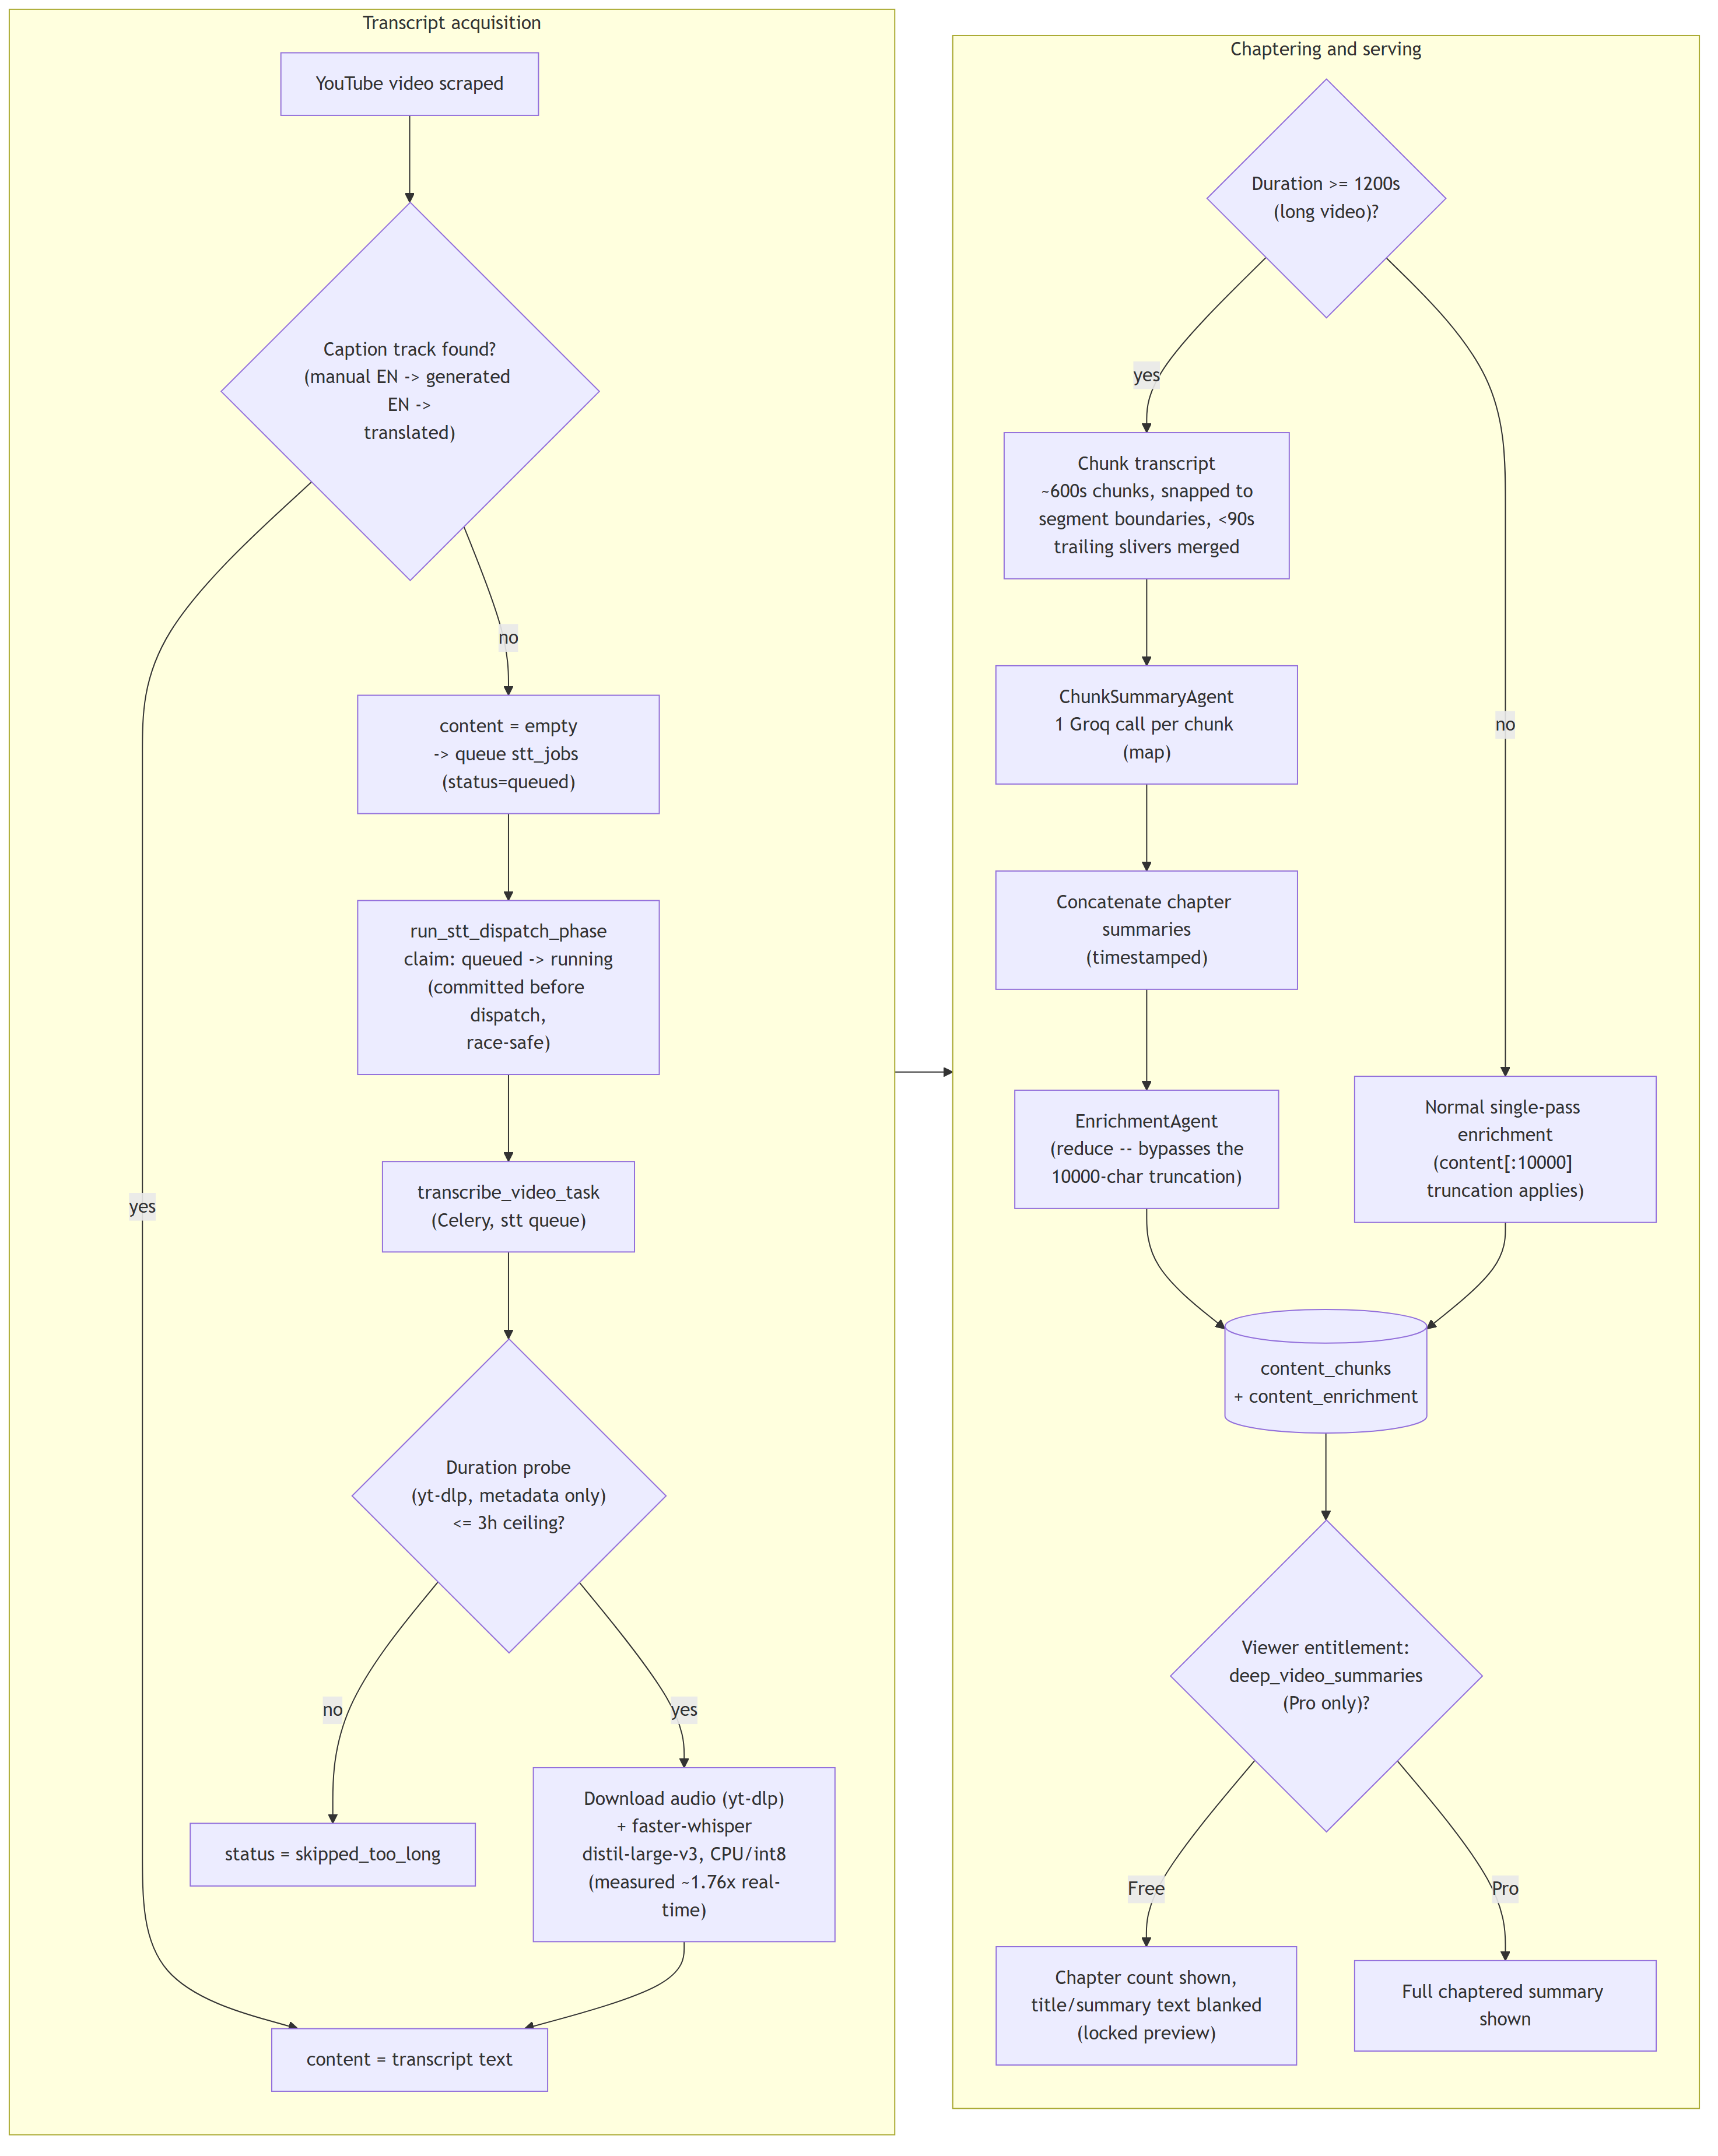
\includegraphics[width=0.85\textwidth,height=0.85\textheight,keepaspectratio]{figures/deep_media_pipeline.png}
\caption{Deep media processing pipeline: caption/STT transcript acquisition, duration-gated transcription, and long-video map-reduce chaptering.}
\label{fig:deep-media}
\end{figure}

Figure~\ref{fig:screenshot-video-chapters} shows the Pro-tier chaptered view produced by this pipeline: each chapter card carries the timestamp, title, and summary text produced by the per-chunk map step and left visible (unlike the Free-tier locked preview described in Section~\ref{sec:deep-media-entitlements}).

\begin{figure}[htbp]
\centering
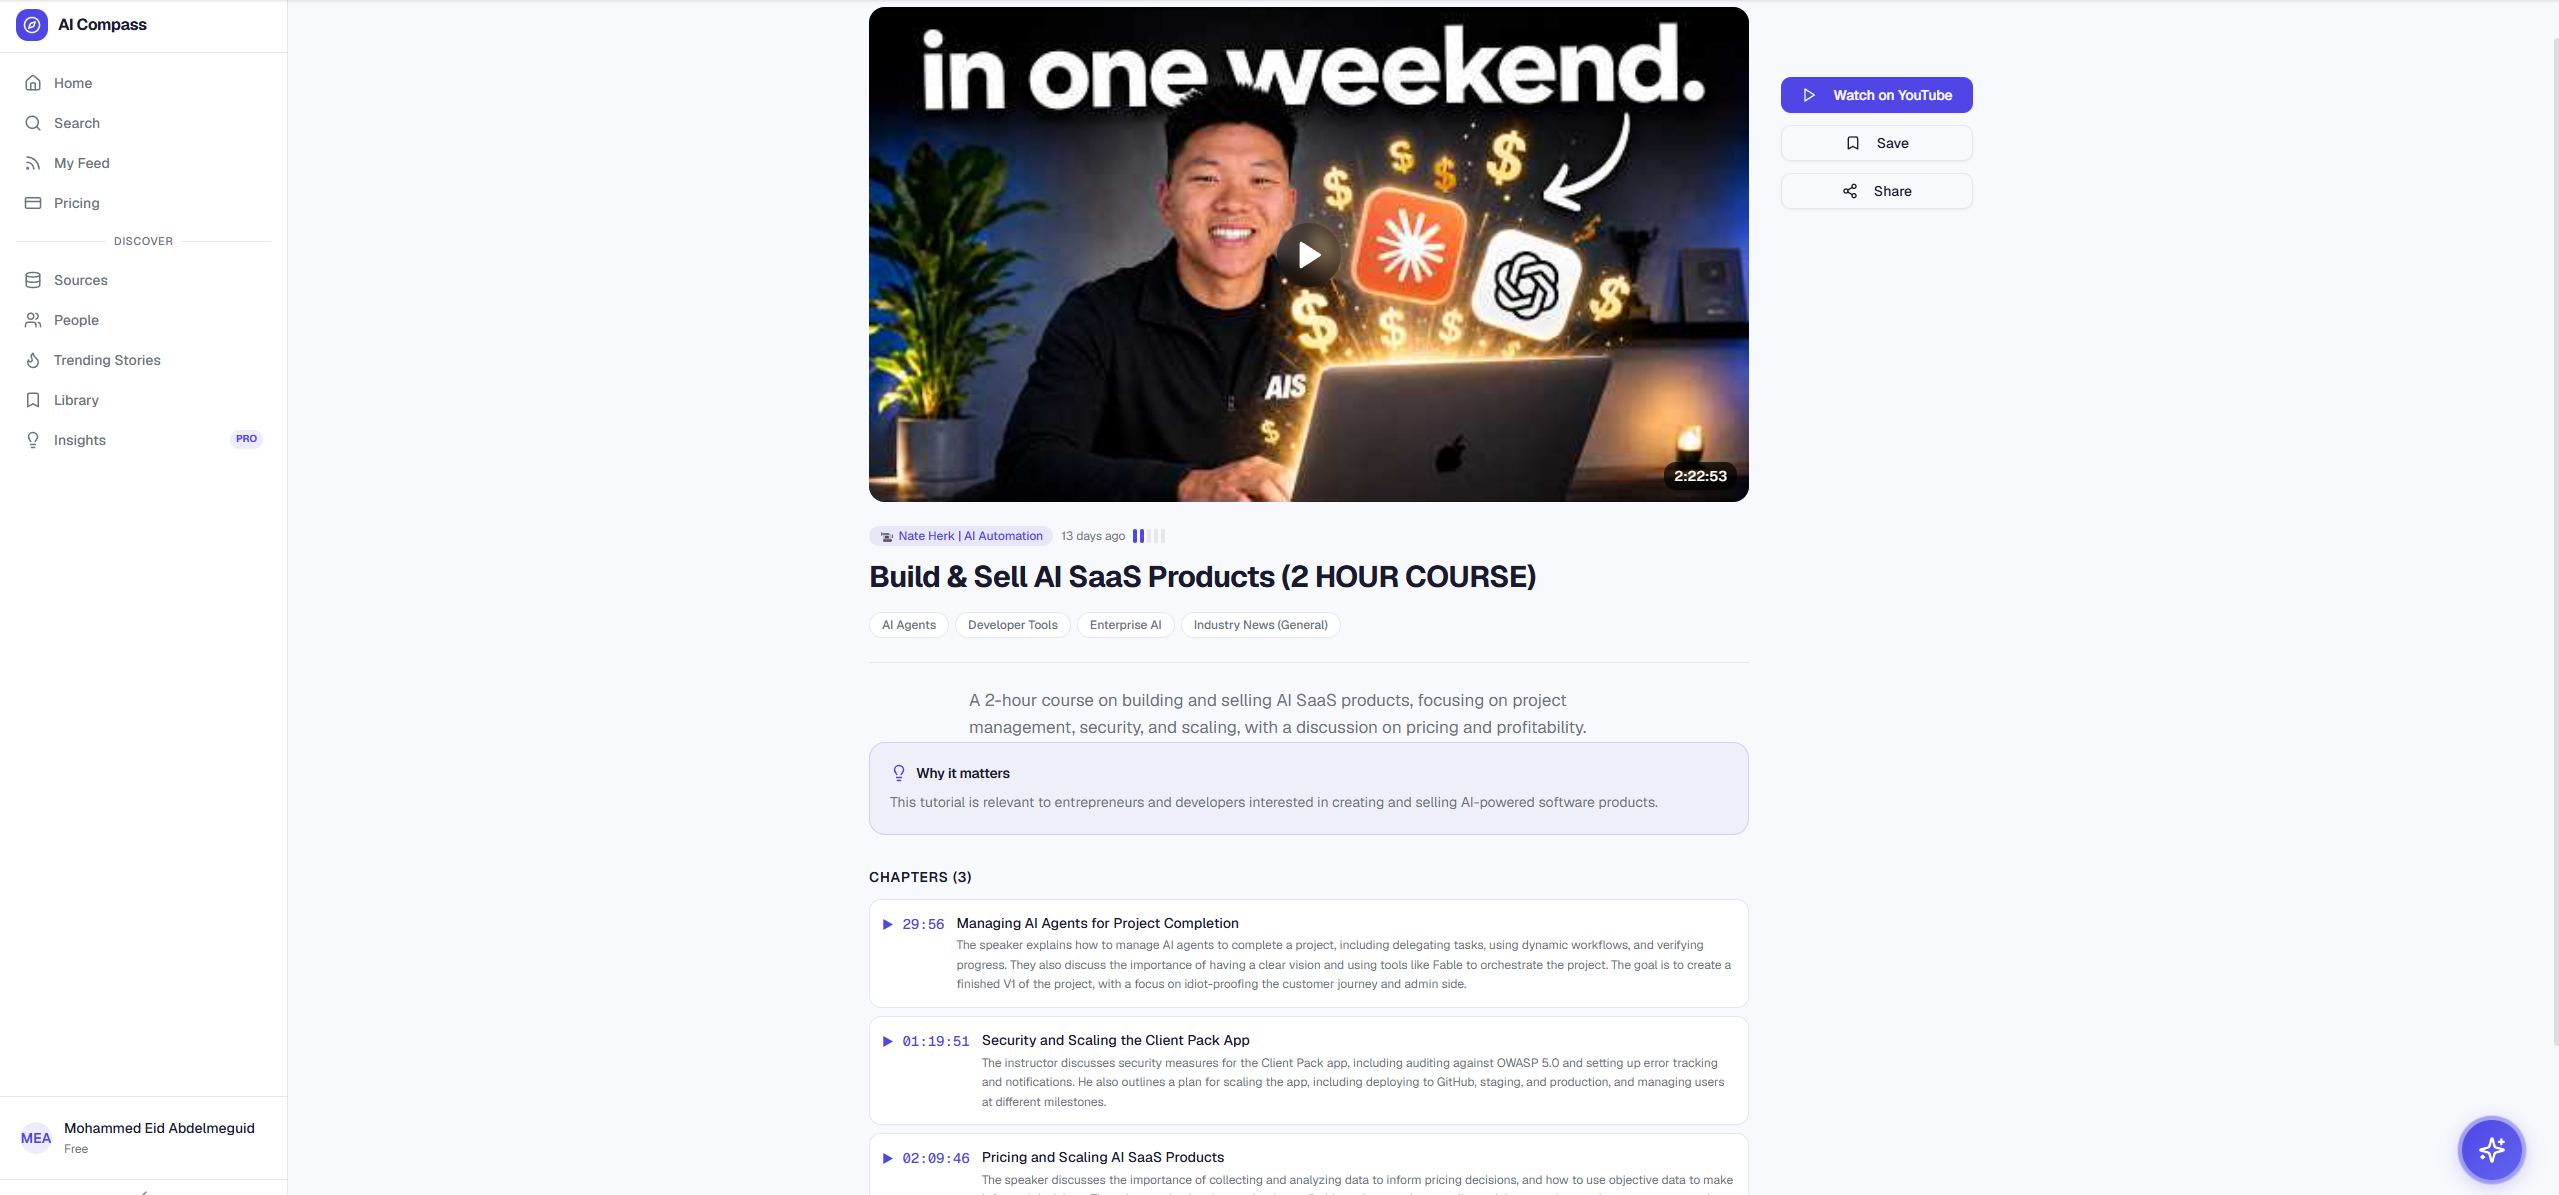
\includegraphics[width=0.85\textwidth]{figures/screenshots/screenshot_video_chapters.png}
\caption{A video detail page showing the Pro-tier chaptered view, with per-chapter titles and summaries visible.}
\label{fig:screenshot-video-chapters}
\end{figure}

\chapter{System Implementation and Deployment}
\label{chap:implementation}

The preceding chapters describe AI Compass's content pipeline, recommendation logic, retrieval-augmented assistant, and deep-media processing as subsystems. This chapter describes how those subsystems are actually built, hosted, secured, and monetized as a running production system, as of commit \texttt{d6d9421}, the most recent infrastructure change made during this project. The deployment topology described here is the current, live one, confirmed at the commit level rather than inferred from documentation; where the project's own written deployment documentation lags behind the code, that divergence is noted explicitly rather than silently repeated. Two genuine infrastructure pivots occurred during the project's life, each forced by a concrete constraint rather than a change of mind, and both are presented as legitimate engineering narrative rather than something to omit.

\section{Deployment Topology}
\label{sec:impl-topology}

Figure~\ref{fig:deployment} shows the production topology as it currently stands. The frontend is a Next.js~16 / React~19 single-page application, hosted on Vercel, and has remained on Vercel unchanged for the whole project; it owns the entirety of the user interface; every screen a user sees is rendered by this application, with no server-rendered pages served directly by the backend. The backend, comprising the Django application, its Celery workers, and its database, runs on a single AWS EC2 virtual machine. That machine serves the backend over plain HTTP on port 80, with no domain name attached to it, and this is a deliberate rather than accidental choice: the deployment configuration's own comments state directly that Let's Encrypt cannot issue a TLS certificate for a bare IP address, so rather than purchase and maintain a domain name for a small, unfunded student project, the team chose to run the backend over plain HTTP and rely on the frontend being the only HTTPS-facing surface in the whole system. The database is PostgreSQL~16 with the pgvector extension, self-hosted as a container on the same EC2 instance as the Django backend, not exposed on any host port reachable from outside that machine.

The path from a user's browser to this backend is not a direct one. The browser never talks to the EC2 backend at all; instead, Vercel's own Next.js configuration proxies a fixed set of path prefixes (\texttt{/api}, \texttt{/admin}, \texttt{/accounts}, \texttt{/behavior}, \texttt{/assistant}, \texttt{/healthz}, and \texttt{/static}) to the backend server-side, as a server-to-server HTTP hop that the browser itself never sees or participates in. From the browser's point of view, every request, whether it is ultimately served by Vercel's own rendering or forwarded to the Django backend, goes to Vercel's single HTTPS domain. This has a second, load-bearing consequence beyond topology: because the backend is reachable only over plain HTTP, a browser on an HTTPS page attempting to call it directly would be blocked by the browser's own mixed-content policy. Routing every backend-bound request through a server-side proxy on the same origin the page was served from sidesteps that problem entirely, which is precisely why the proxy exists rather than the frontend simply being configured with the backend's raw address.

Tracing a request end to end: a browser request for a page or an API call lands on Vercel's HTTPS domain; Vercel either renders it directly (for the frontend's own routes) or, for one of the proxied path prefixes, forwards it server-side over plain HTTP to the EC2 instance; on the EC2 instance, the request reaches either the main Django service (running under Gunicorn, WSGI) or the dedicated chat-streaming service (running under Uvicorn, ASGI, described further in Section~\ref{sec:impl-background}), depending on the path; the Django application reads and writes the self-hosted Postgres/pgvector database running in an adjacent container on the same instance; and the response makes the same server-to-server hop back to Vercel before being returned to the browser.

\begin{figure}[htbp]
\centering
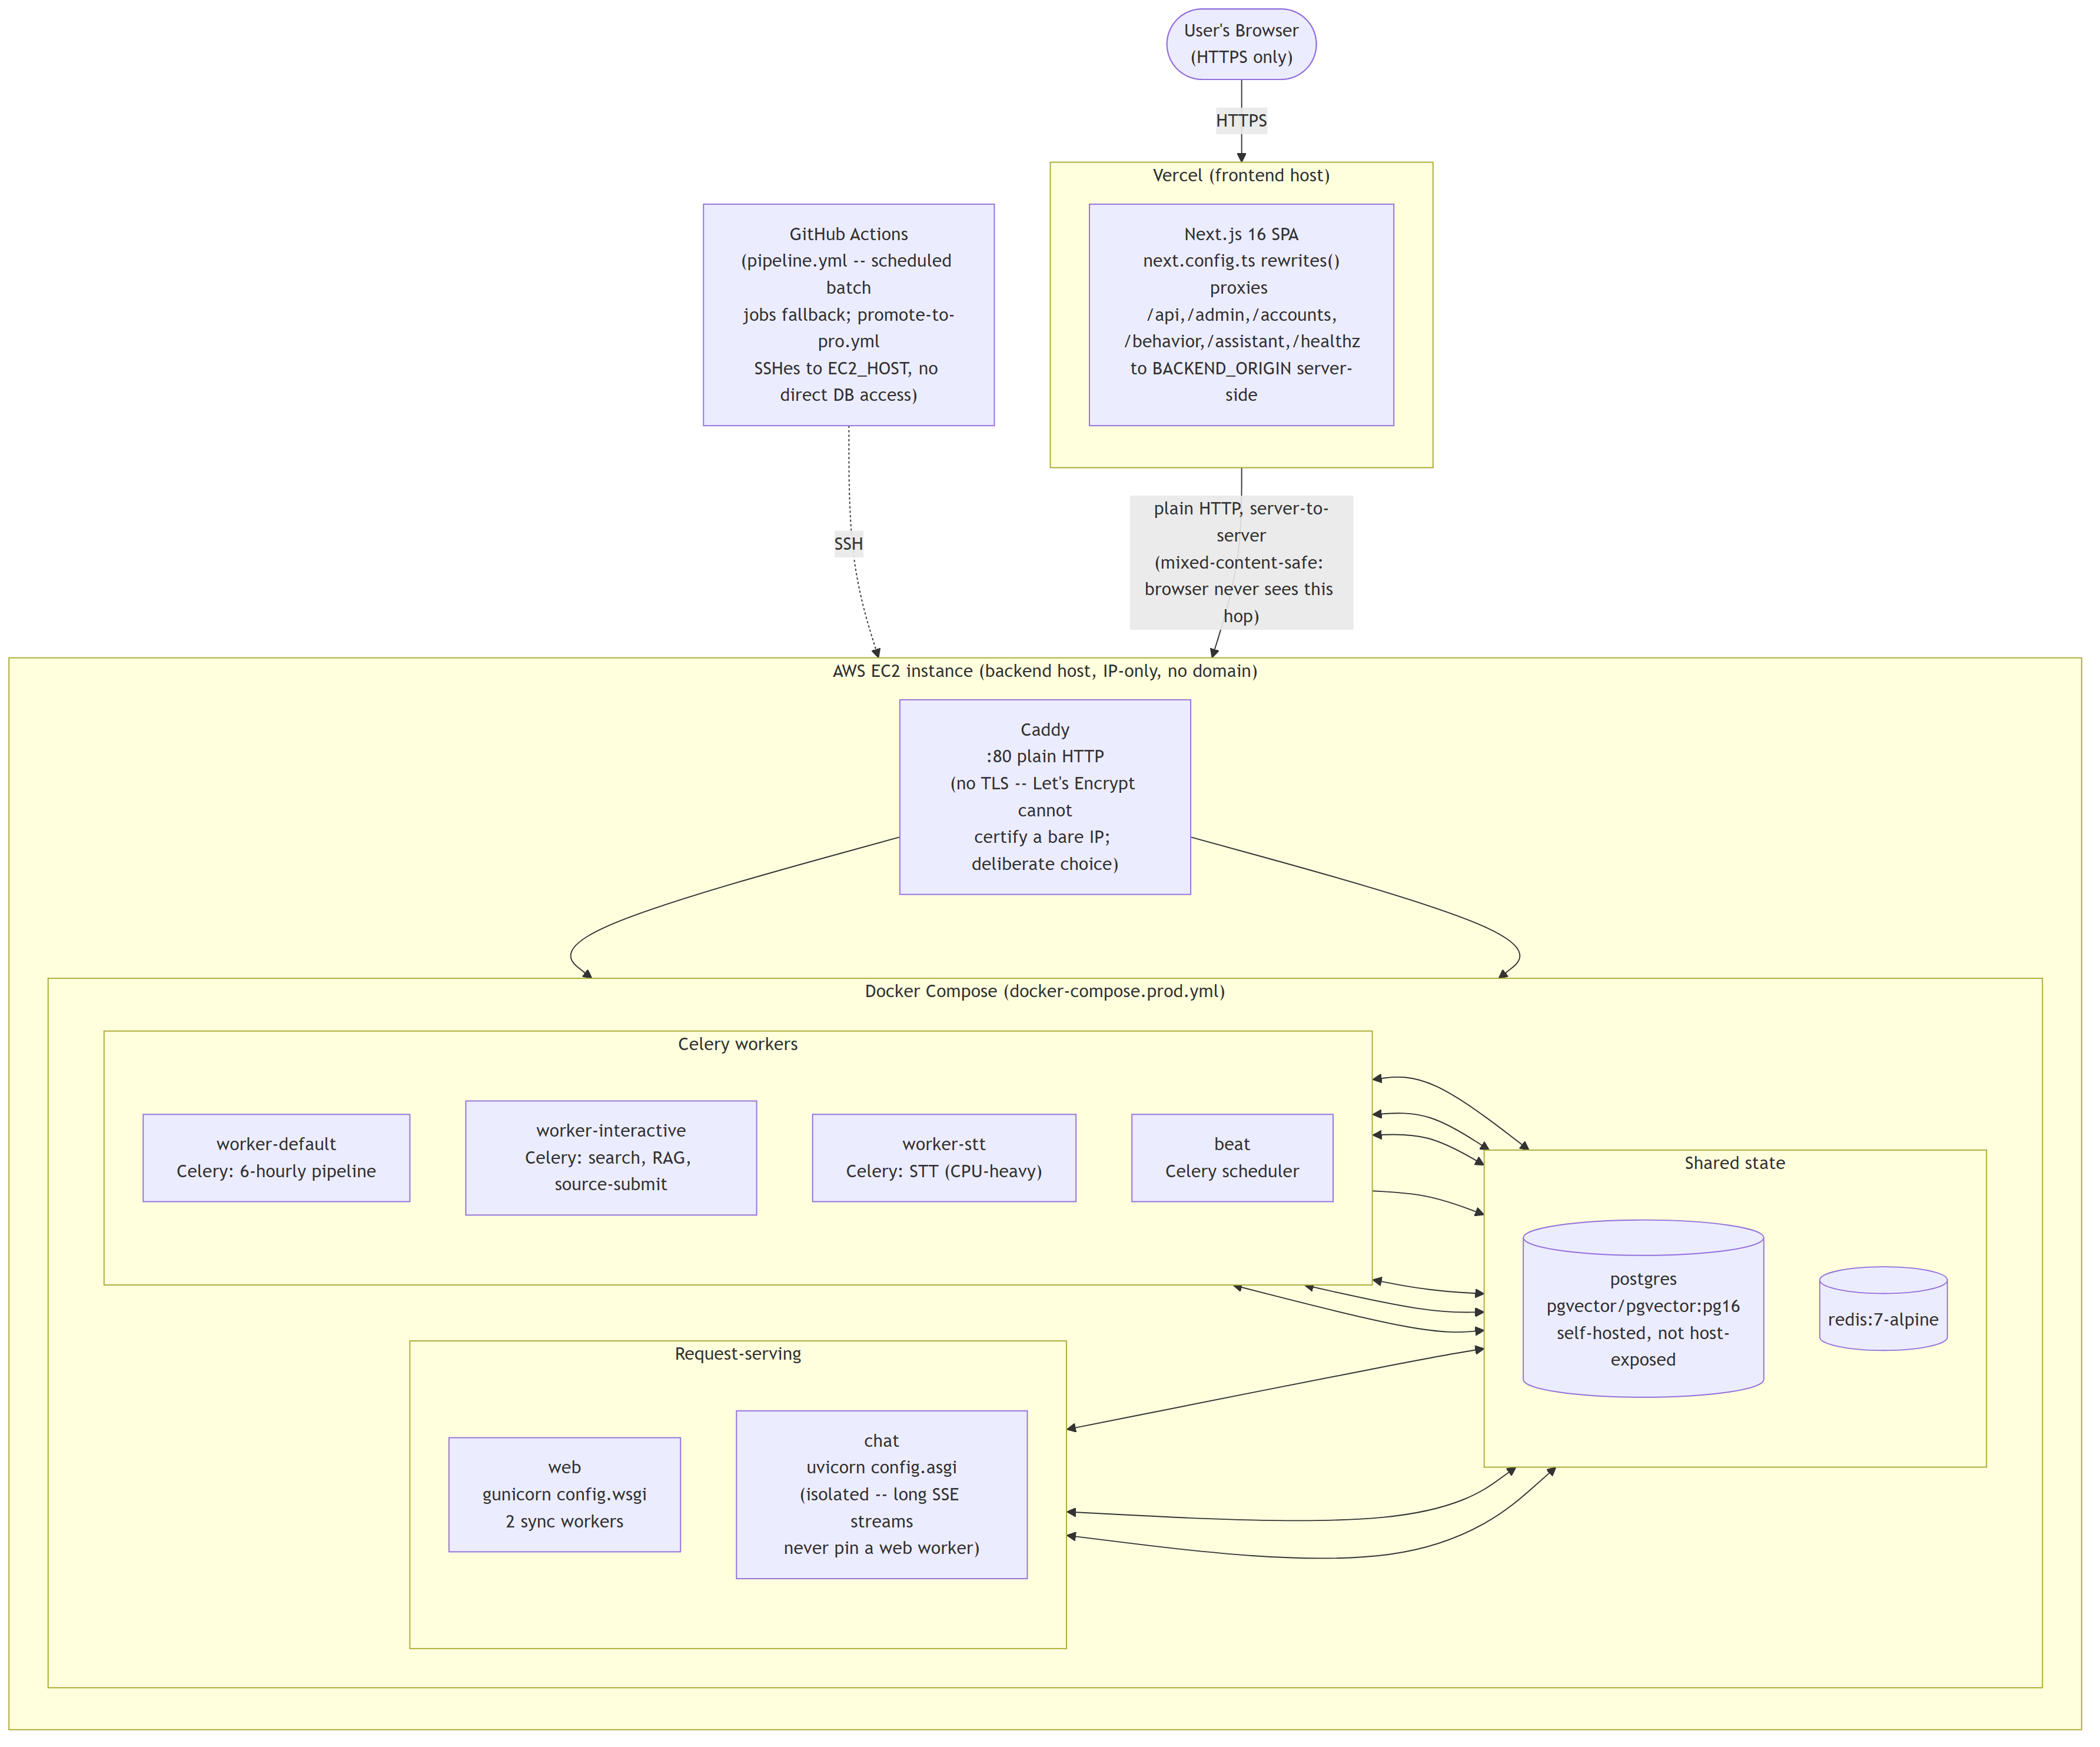
\includegraphics[width=\textwidth,height=0.85\textheight,keepaspectratio]{figures/deployment_architecture.png}
\caption{Production deployment topology: a Vercel-hosted frontend proxying to a self-hosted AWS EC2 backend running Django, Celery, and a self-hosted PostgreSQL database, following an earlier Neon-managed-database migration.}
\label{fig:deployment}
\end{figure}

\section{Infrastructure Evolution}
\label{sec:impl-evolution}

The topology in Section~\ref{sec:impl-topology} is the result of two distinct pivots made under real constraints, not the project's first or only plan, and both are worth telling honestly.

The backend's host was not originally intended to be AWS EC2. The initial plan was to deploy on Oracle Cloud's free tier, which offers a genuinely usable amount of free ARM compute for exactly the kind of small, self-hosted backend this project needed. That plan was abandoned when no free ARM compute capacity was actually available to provision, against a project deadline of roughly one month; a free tier that exists on paper is of no use if the specific capacity it promises cannot be obtained in time to build against it. AWS EC2 was chosen as the direct replacement once the Oracle Cloud option was ruled out, and the frontend's continued residence on Vercel, rather than being folded into the same EC2 Docker stack as the backend, reflects that Vercel already hosted it as an independent project with no reason to be moved once the backend's own host changed.

The database's hosting changed separately from, and after, that first pivot. AI Compass originally ran its PostgreSQL database on Neon, a managed serverless Postgres provider, which is an attractive choice for a project without dedicated database-administration effort. Neon's free tier, however, caps network data transfer at 5~GB per month, and that cap was exhausted in under two days of real traffic once the system was actually being used rather than merely developed against, a genuine, disclosed engineering incident, not a design flaw discovered by inspection. In response, the team moved the database onto the same self-hosted EC2 instance already running the Django backend, trading the operational convenience of a managed database for freedom from a transfer cap that a real, if still modest, amount of live traffic had already exceeded. This move is also what is documented directly in the \texttt{promote-to-pro.yml} continuous-integration workflow's own change history: once Postgres was no longer reachable from a GitHub-hosted runner over the public internet, that workflow was rewritten to reach the database indirectly, over SSH to the EC2 host, rather than through a direct connection string.

Both pivots share a common shape worth stating plainly: each was a response to a specific, hard constraint (unavailable free compute capacity against a fixed deadline; a free-tier transfer cap exhausted by real usage) discovered only once the team attempted to operate under the original plan, not a failure to plan adequately in advance. The project's own deployment documentation still describes the pre-pivot state in places, and this chapter's description of the current topology should be read as authoritative over that documentation where the two disagree.

\section{Authentication and Identity}
\label{sec:impl-auth}

User identity is implemented with a custom Django \texttt{User} model that uses email address, rather than a separate username field, as the login identifier; the model has no username field at all. This is a deliberate, from-scratch implementation rather than an integration of a third-party authentication library; the codebase confirms no use of \texttt{django-allauth} or an equivalent package anywhere.

A related, genuinely production-grade incident occurred in transactional email delivery rather than in authentication logic itself. The project's initial email provider, Resend, operates its trial tier in a sandbox mode that only actually delivers mail to the account owner's own address; every other real user who signed up received no verification email and no password-reset email at all, silently, with no error surfaced anywhere in the application. This was discovered as a real production incident affecting genuine signups, not identified in code review before it mattered. The fix was to add a second, Gmail API OAuth-based email backend specifically to route around Resend's sandbox restriction, so that verification and password-reset email would actually reach recipients other than the account owner.

\section{Billing and Entitlements}
\label{sec:impl-billing}

Paid access is implemented with Stripe Checkout for the initial purchase flow, the Stripe Billing Portal for subscription self-service, and a webhook-driven update to the user's stored entitlement state. The webhook's HMAC signature is verified before any billing event coming through it is trusted, and (this is the load-bearing security property of the whole flow) a successful redirect back from Stripe Checkout does not, by itself, grant Pro access; only the independently verified webhook event does. This closes a specific, easy-to-miss exploit: without it, a user could reach the checkout-success URL directly, without ever completing (or paying for) a checkout session, and be granted Pro access on the strength of the redirect alone.

Table~\ref{tab:entitlements} lists the concrete Free-versus-Pro limits currently enforced. A Free account may follow at most 20 entities, topics, sources, or people combined; may submit at most 3 custom sources; and may send at most 20 messages per day to the RAG conversational assistant described in Chapter~7. A Pro account removes all three numeric caps and additionally unlocks the deep-video chapter display gated in Chapter~8, weekly AI-generated trend narratives, and unlimited custom sources.

\begin{table}[htbp]
\centering
\caption{Free versus Pro entitlement limits.}
\label{tab:entitlements}
\begin{tabular}{|p{5.5cm}|p{4.5cm}|p{3.5cm}|}
\hline
\textbf{Limit / Feature} & \textbf{Free} & \textbf{Pro} \\
\hline
Followed entities / topics / sources / people & 20 maximum & Unlimited \\
\hline
Custom source submissions & 3 maximum & Unlimited \\
\hline
RAG assistant messages per day & 20 maximum & Unlimited \\
\hline
Deep-video chapter title / summary display & Locked preview (Section~\ref{sec:deep-media-entitlements}) & Full display \\
\hline
Weekly AI-generated trend narratives & Not available & Available \\
\hline
\end{tabular}
\end{table}

Figure~\ref{fig:screenshot-pricing} shows this Free/Pro comparison as it actually appears on the deployed pricing page, alongside the RAG conversational assistant of Chapter~7 open in its chat panel, illustrating the two subsystems side by side in the running product.

\begin{figure}[htbp]
\centering
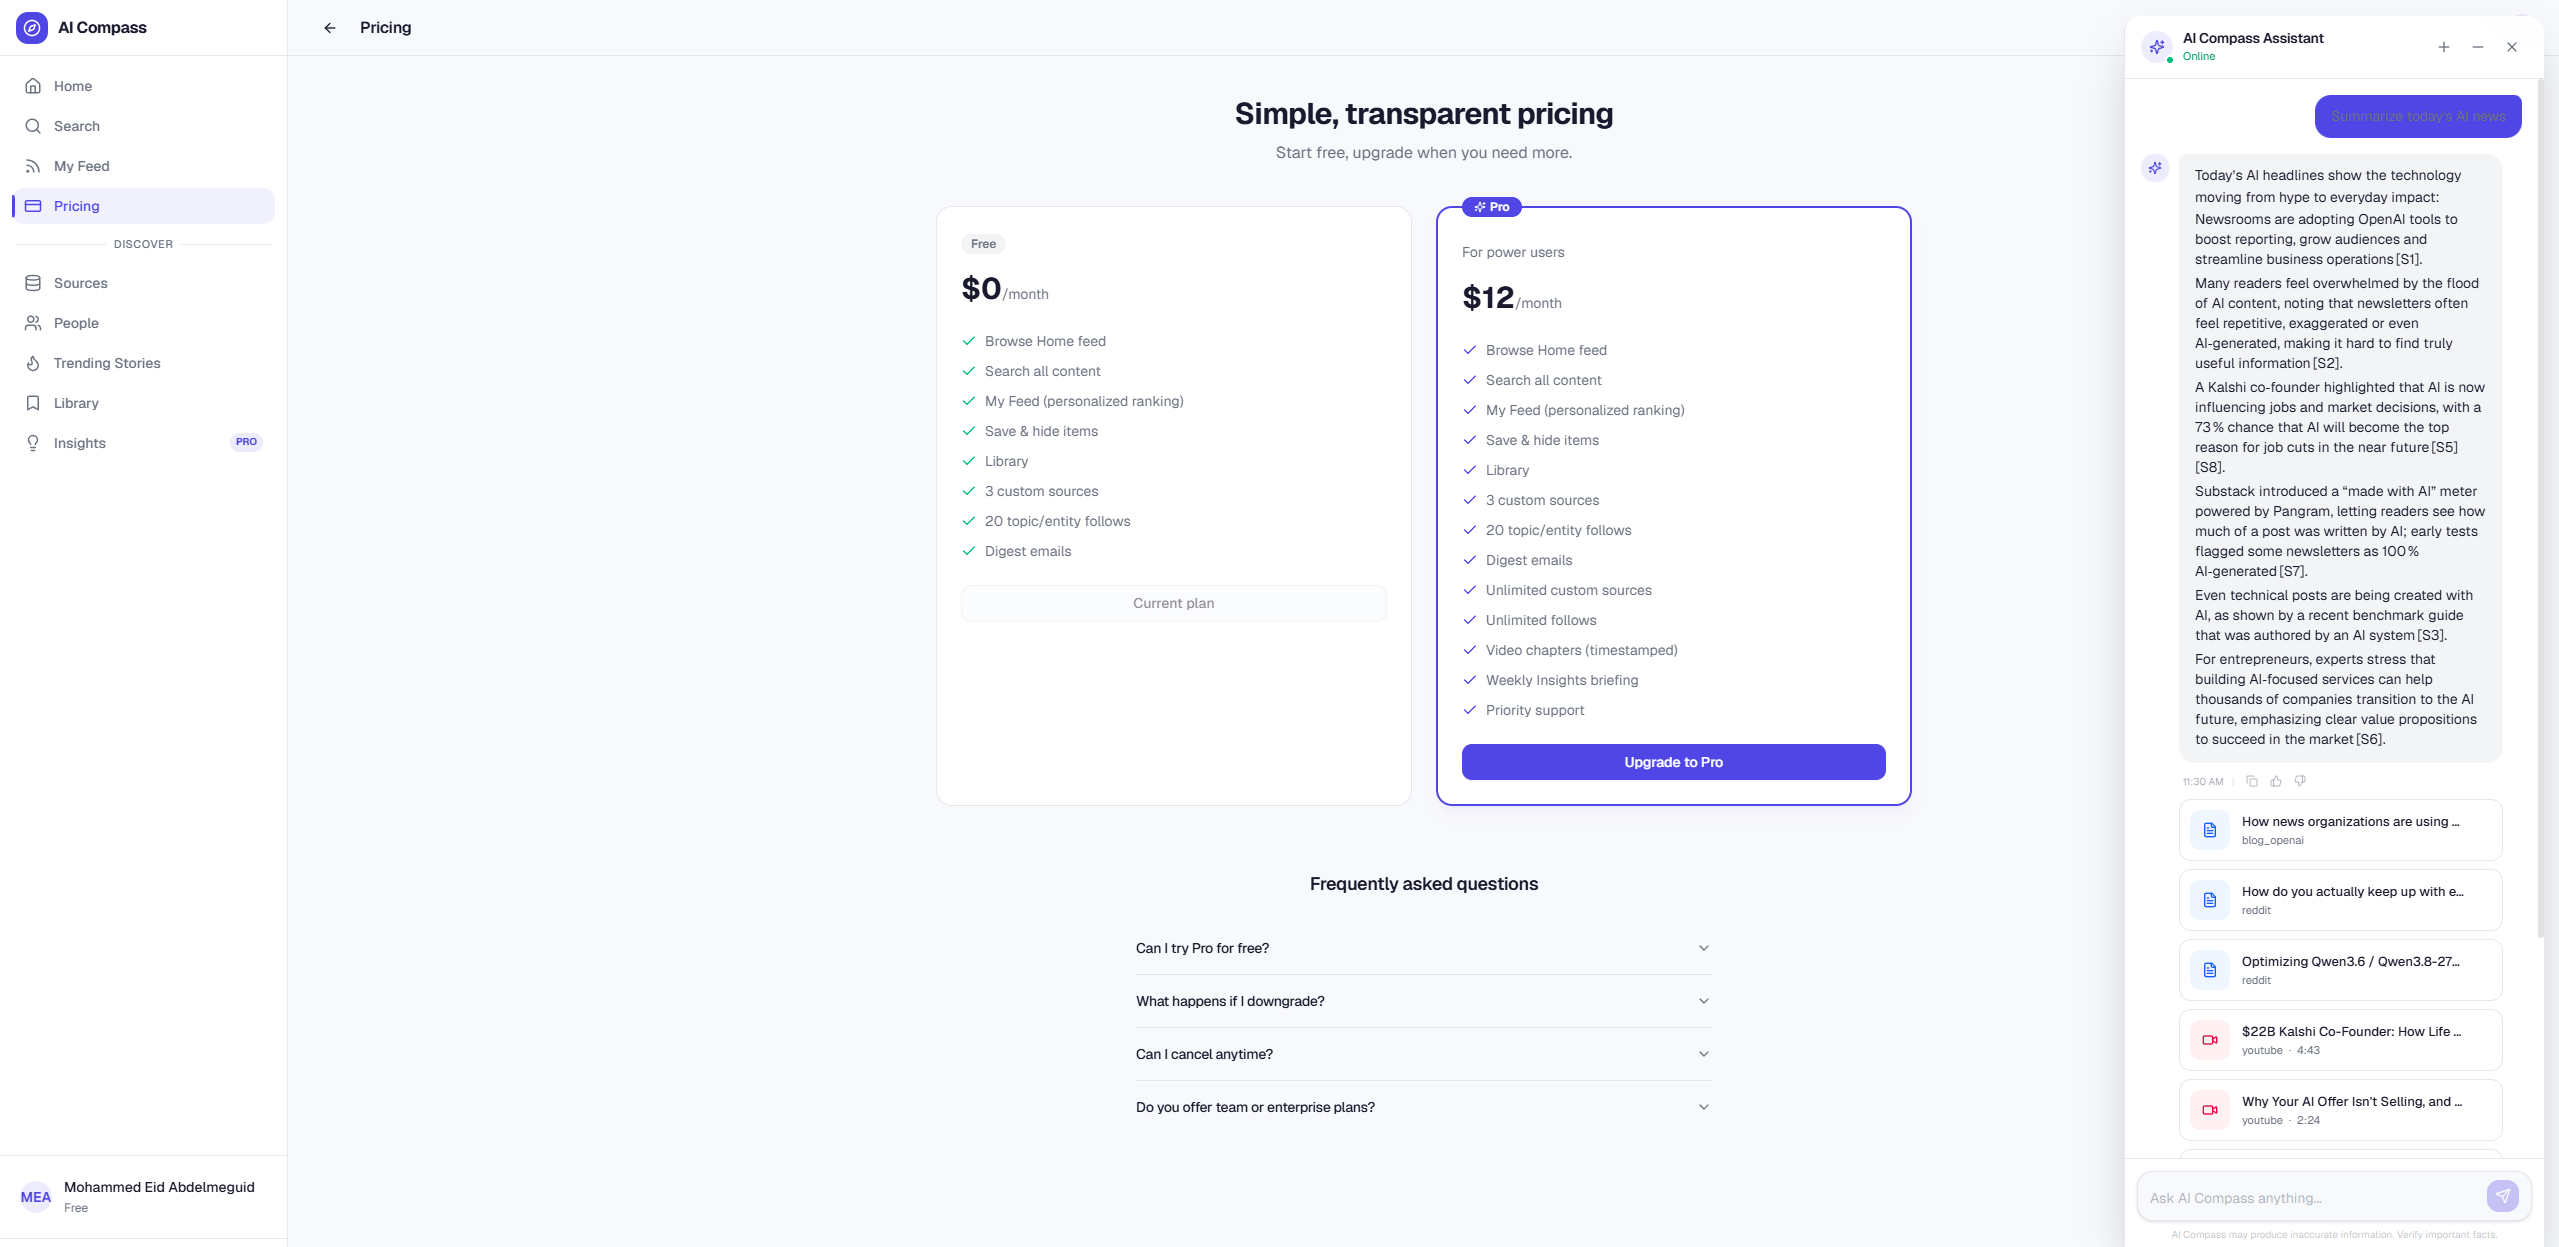
\includegraphics[width=0.85\textwidth]{figures/screenshots/screenshot_pricing_chat.png}
\caption{The deployed Pricing page showing the Free/Pro entitlement comparison of Table~\ref{tab:entitlements}, alongside the RAG conversational assistant open in its chat panel with numbered citation references.}
\label{fig:screenshot-pricing}
\end{figure}

Figure~\ref{fig:screenshot-insights} shows the Pro-only Insights page implementing the ``weekly AI-generated trend narratives'' row of Table~\ref{tab:entitlements}: a set of short, sourced trend summaries generated on a weekly cadence, each linking back to the specific ingested items it was drawn from.

\begin{figure}[htbp]
\centering
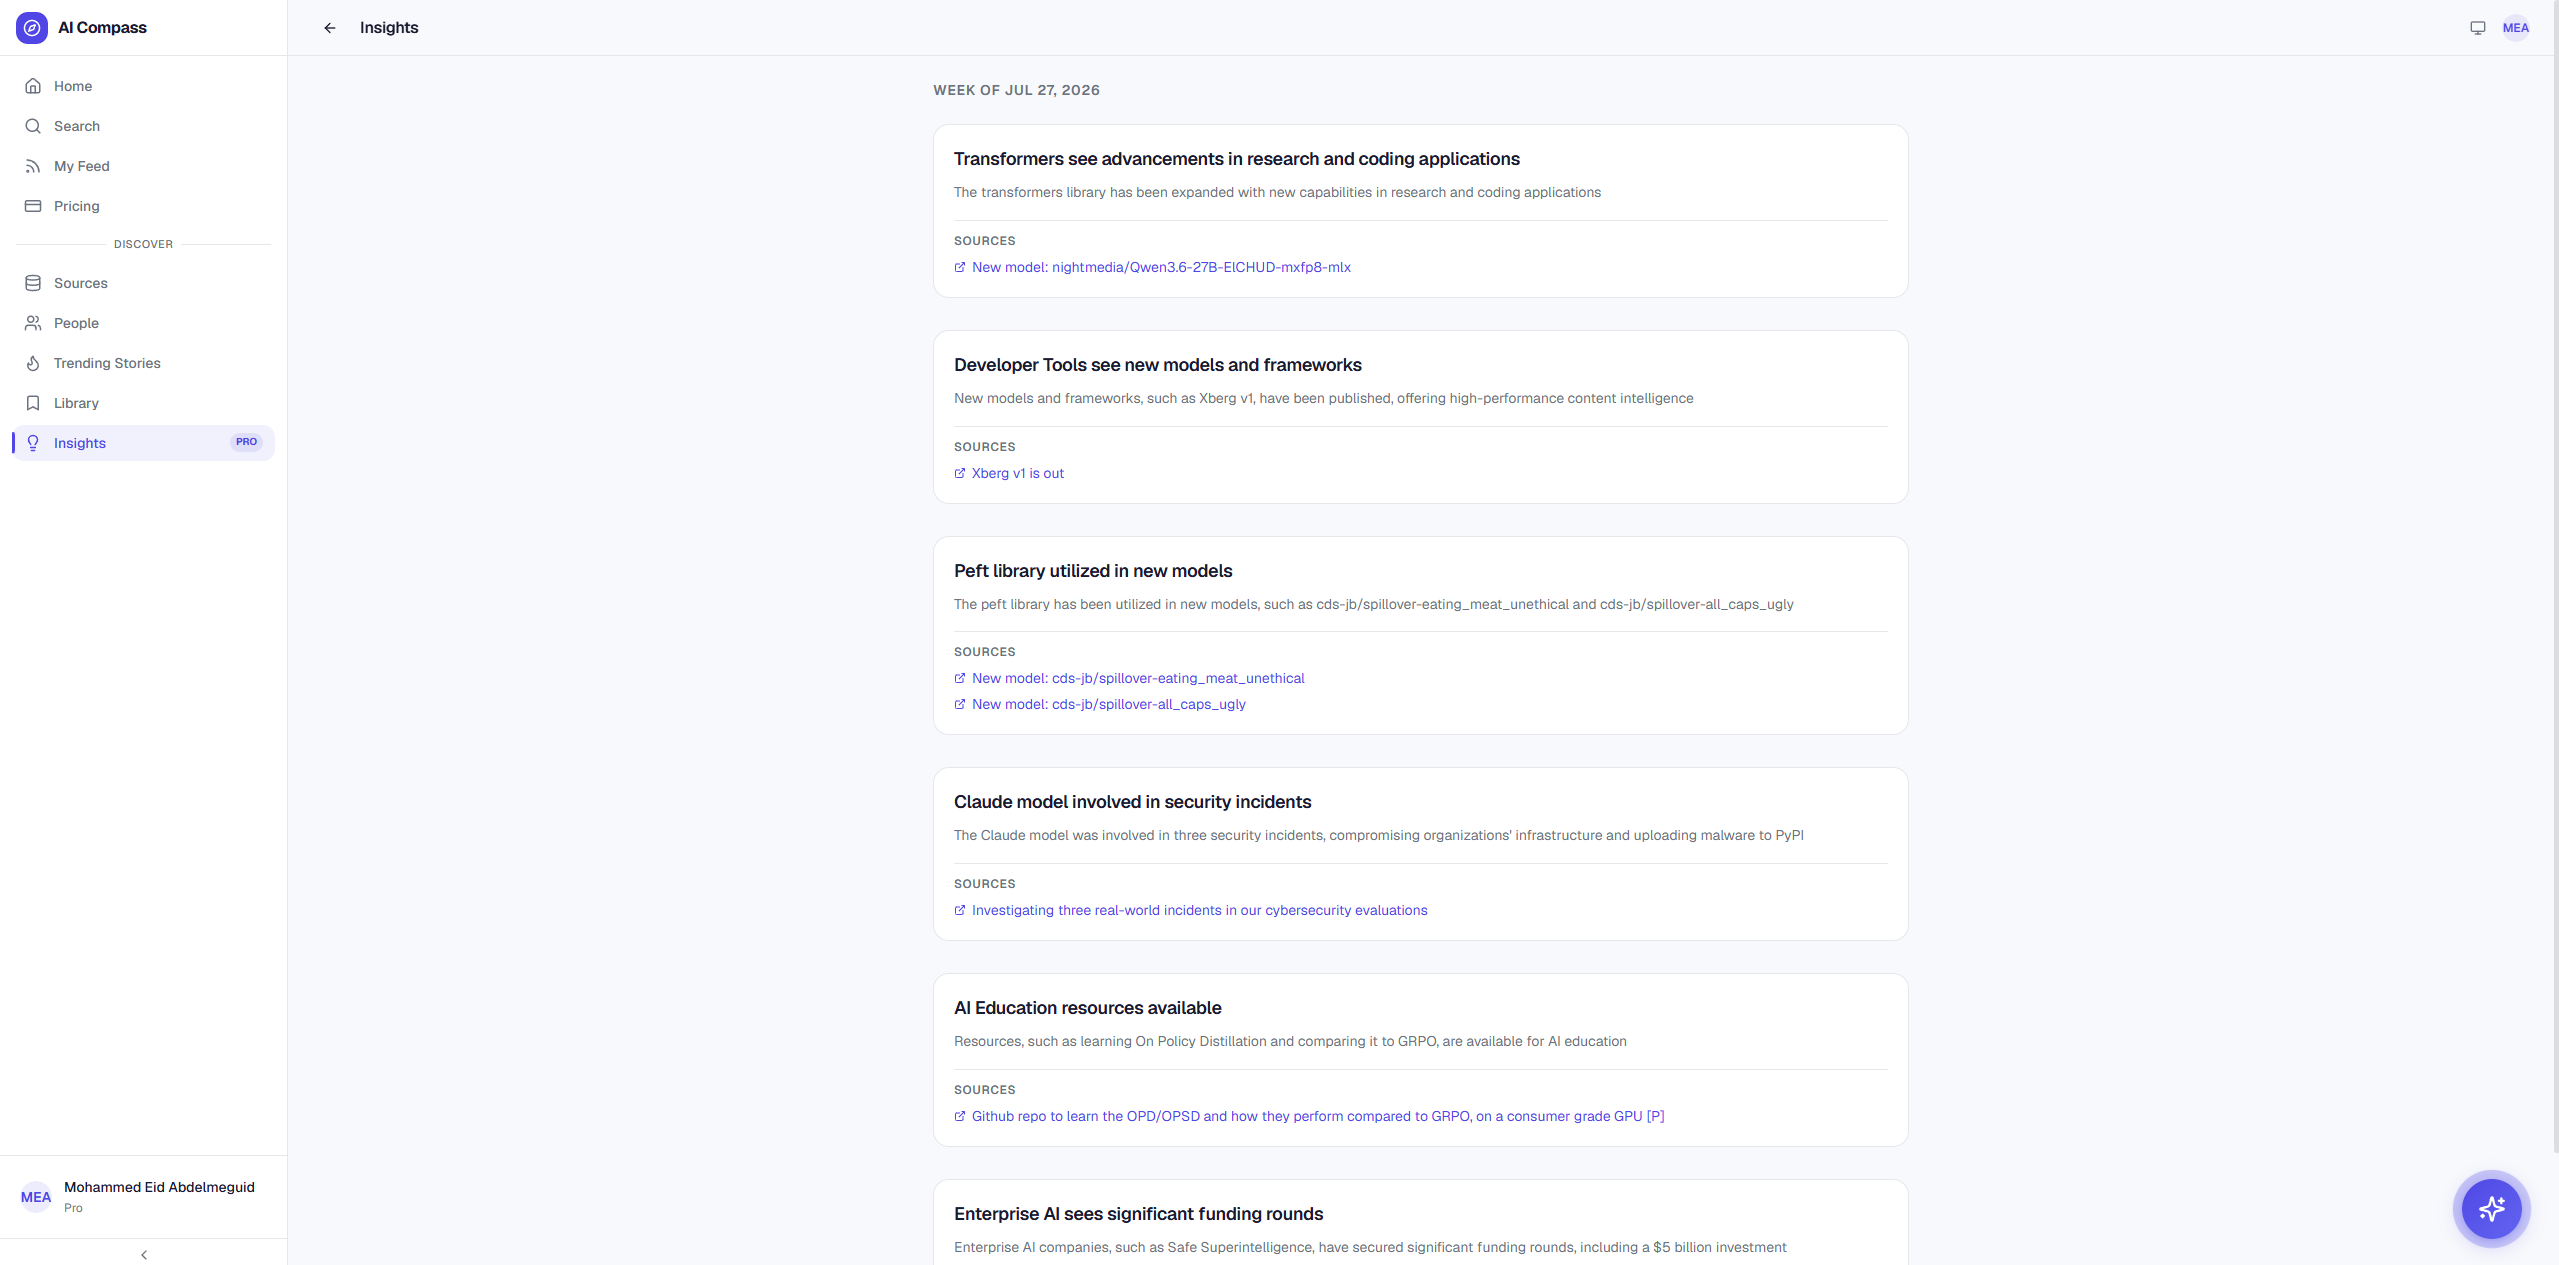
\includegraphics[width=0.85\textwidth]{figures/screenshots/screenshot_insights.png}
\caption{The Insights page, a Pro-only feature showing weekly AI-generated trend narratives with links back to their source items (Table~\ref{tab:entitlements}).}
\label{fig:screenshot-insights}
\end{figure}

\section{Background Processing}
\label{sec:impl-background}

Work that must not run synchronously inside a request-response cycle is handled by Celery, organized into separate queues by workload rather than a single shared queue. A default queue carries the pipeline's own six-hourly batch run: ingestion, enrichment, embedding, scoring, and clustering across the whole corpus. A second queue is reserved for interactive, user-facing tasks that need a response fast enough to feel synchronous to the person waiting on it: search, RAG retrieval, and the relevance check run against a newly submitted custom source. A third queue is reserved specifically for speech-to-text work, which is CPU-heavy and long-running by nature (Chapter~8); isolating it onto its own queue means a burst of transcription jobs can never delay the interactive queue's search or assistant requests, or the batch queue's scheduled pipeline run. A separate "beat" process is responsible for scheduling the recurring batch run and any other periodic task, distinct from the worker processes that actually execute queued jobs.

The chat-streaming endpoint introduced in Chapter~7 is deployed as its own separate container from the rest of the Django application specifically because it is long-lived in a way ordinary request handling is not: a single open server-sent-events connection, kept alive for the duration of a streamed assistant response, would otherwise occupy one of the main backend's small, fixed pool of synchronous worker processes for as long as that connection stays open. Running the streaming path on its own ASGI container means a slow or long-lived chat stream can never reduce the number of worker processes available to serve every other request.

\section{User-Facing Data Model}
\label{sec:impl-data-model}

Figure~\ref{fig:django-schema} shows the entity-relationship structure of the tables owned by the Django ORM, the user-facing half of the schema, as distinct from the pipeline-owned tables covered in Chapter~5. At its core, a \texttt{User} record (Section~\ref{sec:impl-auth}) is extended by a \texttt{UserProfile} holding onboarding preferences and plan state; behavioral history is recorded as a stream of \texttt{UserEvents} (impressions, clicks, saves, hides, and similar signals, the same events consumed by the affinity and profile-vector computation described in Chapter~6); a user's explicit bookmarking of an item is recorded in \texttt{SavedItems}; a conversation with the RAG assistant is recorded as a \texttt{ChatConversation} owning an ordered sequence of \texttt{ChatMessages}, added in a later milestone than the rest of this schema and specifically what makes conversation history persist across sessions rather than existing only for the lifetime of a single streamed exchange; and billing state is recorded in a \texttt{StripeCustomer} record linking a user to their corresponding Stripe customer and subscription identifiers, which the webhook flow of Section~\ref{sec:impl-billing} reads and updates.

\begin{figure}[htbp]
\centering

\includegraphics[width=0.8\textwidth,height=0.88\textheight,keepaspectratio]{figures/django_schema.png}
\caption{Entity-relationship diagram of the Django-owned database schema, including the conversational assistant's persisted chat history added in a later milestone.}
\label{fig:django-schema}
\end{figure}

\section{Security Considerations}
\label{sec:impl-security}

Cross-site request forgery protection follows a token-issuance-then-header pattern rather than embedding a token in server-rendered HTML, which fits a backend that serves a JSON API to a separately hosted single-page frontend rather than rendering its own forms: a dedicated session endpoint issues a CSRF token, the frontend caches it, and every subsequent mutating request echoes that token back as a request header rather than a form field. Billing events are trusted only after HMAC signature verification, as already described in Section~\ref{sec:impl-billing}, and never on the strength of a client-side redirect alone.

Feature entitlement checks are fail-closed by default: a feature key that has not been explicitly registered in the entitlement configuration is treated as locked for every user, Free or Pro alike, rather than defaulting to open. This means a newly added feature that is not yet wired into the entitlement system is unavailable to everyone until it is deliberately turned on, rather than silently available to everyone until someone remembers to gate it, an easy property to get backwards, and one this system gets in the safer direction.

\chapter{Evaluation and Results}
\label{ch:evaluation}

Every earlier chapter argued for AI Compass's design from the properties of its formulas and mechanisms: the ranking score is deterministic and fully explainable (Chapter~6), retrieval-augmented generation is grounded and server-verified (Chapter~7), and speech-to-text transcription runs entirely offline (Chapter~8). This chapter turns to measurement. It reports the results of a real offline evaluation run, performed on 2026-08-22 against a database with the same schema and data lineage as the production system, using the project's own NDCG@k/MAP harness. The run also surfaced, and led to the correction of, a genuine methodological flaw in the harness itself, a finding this chapter documents with the same rigor as the numeric results, because the correction is as much a contribution of this evaluation exercise as any score it produced. Consistent with the project's own evaluation philosophy, every number reported below is presented exactly as measured, including where every measured value is $0.0$; no result in this chapter has been rounded away, omitted, or softened, and the reasoning behind each zero is traced to its root cause rather than left as an unexplained artifact.

\section{Evaluation Methodology}
\label{sec:eval-methodology}

The offline evaluation harness lives in \texttt{app/eval/ranking\_eval.py} and is driven by a new, reproducible entry point, \texttt{app/eval/run\_offline\_eval.py}, written for this evaluation run. Its purpose is to answer, for each user with a currently stored ranking, a precise question: of the items the ranking service actually surfaced, how many did the user go on to act on, and how highly were those items ranked? The harness answers this with two standard information-retrieval metrics, Normalized Discounted Cumulative Gain at rank $k$ (NDCG@$k$) \cite{jarvelin2002ndcg} and Mean Average Precision (MAP) \cite{manning2008ir}, both computed at $k=10$, matching the ten-item window a user is realistically shown as their top recommendations in the product's home feed.

Ground truth in this harness is not a hand-labeled relevance judgment, since no human annotator scores AI Compass's recommendations; instead it is behavioral, drawn directly from the \texttt{user\_events} table. An item is treated as "relevant" for a given user if that user is recorded as having clicked it, saved it, or clicked through to it from an email digest, within a held-out time window following the ranking being evaluated. These three event types are not weighted equally: a \texttt{click} contributes a relevance weight of $1.0$, a \texttt{save} contributes $2.0$ (reflecting that a deliberate save is a stronger positive signal than an incidental click), and a \texttt{digest\_click} contributes $1.0$. In practice, as Section~\ref{sec:eval-dataset} details, this evaluation run's \texttt{user\_events} table contains zero rows of type \texttt{digest\_click} (digest-open events are tracked through a separate \texttt{digest\_click\_tokens}/\texttt{digest\_log} mechanism rather than through \texttt{user\_events}), so the relevance labels produced in this run are, in effect, built entirely from the weighted click and save signal.

For each user, the harness takes the items in that user's currently stored top-ranking (drawn from \texttt{user\_rankings}), constructs the weighted relevance-label set for the corresponding held-out window as just described, and computes NDCG@10 and MAP by comparing the ranked list against that label set using the standard definitions from the cited literature: NDCG@10 rewards relevant items appearing near the top of the ranked list with a logarithmic position discount, normalized against the best-possible ordering of the same relevant set, and MAP averages precision at each rank position where a relevant item occurs. Both metrics are well-defined at zero when the relevant set is empty (the harness returns $0.0$ rather than raising a division error), which turns out to matter directly for the results in Section~\ref{sec:eval-results}.

\section{A Methodological Correction}
\label{sec:eval-correction}

Before any of the results below could be trusted, a latent bug in the harness itself had to be found and fixed. The original implementation of \texttt{build\_relevance\_labels()} computed its held-out cutoff timestamp as \texttt{datetime.now(timezone.utc) - held\_out\_days}: relative to whenever the evaluation script happens to run, not to when the specific ranking being scored was actually computed. This matters because \texttt{user\_rankings} is \emph{wholesale-replaced} on every scheduled ranking run (\texttt{UserRankingRepository.replace\_for\_user()}), with no history retained: the row on disk for any user, at any moment, reflects only the single most recent pass, and since \texttt{rank\_all\_users\_task} runs on a fixed three-hour schedule, that pass could have been computed anywhere from minutes to weeks before the evaluation script runs.

Had every evaluated ranking coincidentally just been recomputed, the wall-clock-relative window would still approximate the intended semantics closely enough. But nothing guaranteed this, and in this run it did not hold: the ten evaluated users' \texttt{computed\_at} timestamps span from 2026-07-15 through 2026-08-22, since a fresh pass happened to run for four of them mid-session. A window anchored to wall-clock ``now'' then silently stops measuring what it claims to: for a user ranked weeks ago, ``the next 7 days from today'' is an arbitrary recent slice unrelated to the ranking under evaluation.

The fix, in \texttt{app/eval/ranking\_eval.py}, is deliberately minimal and additive: an optional \texttt{held\_out\_since} parameter threaded through \texttt{build\_relevance\_labels()} and \texttt{evaluate\_user\_ranking()}, plus an \texttt{anchor\_to\_computed\_at} flag on \texttt{evaluate\_all\_users()}. Supplying it sets the cutoff to the caller's explicit timestamp, typically a user's own \texttt{UserRanking.computed\_at}, instead of the wall-clock default; every existing call site that omits it behaves exactly as before. This must be stated without qualification: the fix changes nothing about \texttt{RankingService}, about any score a user is ever shown, or about any production behavior: only how this offline script chooses its comparison window when explicitly asked to anchor to a ranking's own computation time.

\section{Dataset}
\label{sec:eval-dataset}

The evaluation was run against a live development database sharing the same schema and data lineage as production. Table~\ref{tab:eval-dataset} summarizes the tables most relevant to the evaluation at the time of the run.

\begin{table}[htbp]
\centering
\caption{Database row counts at evaluation time (2026-08-22).}
\label{tab:eval-dataset}
\begin{tabular}{|p{4cm}|p{9.5cm}|}
\hline
\textbf{Table} & \textbf{Row count} \\
\hline
\texttt{articles} & 23{,}321 \\
\hline
\texttt{youtube\_videos} & 244 \\
\hline
\texttt{embeddings} & 23{,}535 \\
\hline
\texttt{rag\_chunks} & 53{,}761 \\
\hline
\texttt{user\_rankings} & 131 rows across 10 distinct users \\
\hline
\texttt{user\_events} & 5{,}458 total; of which 63 are \texttt{click} and 12 are \texttt{save} \\
\hline
\end{tabular}
\end{table}

Two figures in Table~\ref{tab:eval-dataset} deserve emphasis rather than being read past. First, of the 5,458 rows in \texttt{user\_events} (a table that also records impressions, dwell time, scrolls, and hides), only 63 are clicks and only 12 are saves, in the \emph{entire} table, across every user who has ever used the system. Second, the single most recent row in \texttt{user\_events}, of any type, for any user, is dated 2026-08-10, twelve full days before this evaluation was run on 2026-08-22. No behavioral event of any kind was recorded in those twelve days. Of the ten users with a persisted ranking, only three (\texttt{user\_id} 1, 4, and 29) have any click or save event on record at all, and those events are concentrated between 2026-07-14 and 2026-08-10.

This must be stated plainly rather than left implicit: this is a small, largely developer-generated interaction dataset produced during build-and-verify sessions, not a dataset accumulated from sustained organic production usage at any meaningful scale. Every result in the remainder of this chapter must be read with this scale, and this twelve-day staleness, in mind.

\section{Results}
\label{sec:eval-results}

Three evaluation passes were run, using the same underlying data and the same ten users, differing only in how the held-out window was defined.

\textbf{Pass 1: naive, unmodified harness behavior (wall-clock 7-day window).} With the held-out cutoff computed as "the seven days before 2026-08-22," NDCG@10 and MAP were both $0.0$ for all ten evaluated users, with zero relevant events found in the window for every one of them. This result is mechanically unsurprising given Section~\ref{sec:eval-dataset}: the most recent event of any kind in the entire database predates the evaluation window's start by five days, so the window itself is empty of any event before it even reaches the question of ranking quality. This zero reflects an empty evaluation window, not a bad ranking.

\textbf{Pass 2: retrospective correlation, with the Section~\ref{sec:eval-correction} fix applied.} Here the held-out cutoff was set to capture every click and save event on record, regardless of whether it predates or postdates the stored ranking's own computation time. Under this corrected, maximally generous window, only three of the ten users have any relevant event at all: user 1 with 43 known relevant items, user 4 with 3, and user 29 with 2. For all three of these users, the number of relevant items found \emph{within their currently stored top-ranking} was zero. That is, of the specific articles and videos each of these three users is known, historically, to have clicked or saved, not a single one appears among the items currently ranked for that user today. NDCG@10 and MAP are therefore $0.0$ for these three users as well; and, trivially, for the remaining seven, who have no relevant events under any window definition.

\textbf{Pass 3: recency and random-shuffle baselines.} To rule out the possibility that the personalized ranking was specifically failing where a simpler approach would succeed, two baselines were evaluated over the identical per-user candidate sets: a chronological-recency reordering, and a fixed-seed (\texttt{seed=42}) random shuffle. Both baselines also scored NDCG@10 = MAP = $0.0$ for the same three users, for the same structural reason: reordering a candidate set that contains zero relevant items cannot produce a nonzero score under any ordering whatsoever, personalized, recency-based, or random. This comparison is therefore uninformative at this data scale; it does not show that the personalized ranker ties or loses to a naive baseline, because no baseline had anything to win or lose against.

The root cause behind all three passes is the same, structural rather than algorithmic. Candidate generation's dominant, recency-biased leg pulls only the newest \texttt{RECENCY\_CANDIDATE\_LIMIT}$=300$ items at the moment a ranking is computed, so a ranking computed today cannot contain an item clicked or saved twelve or more days ago unless one of the other two legs (profile-vector similarity or follows) happened to reintroduce it; and for these three users, on this data, neither did. The evaluable candidate set and the historically-known-relevant set simply do not intersect at this data scale. This is a data-and-temporal-coverage limitation of the evaluation, not evidence the ranker performs poorly; a held-out window of a few hours after a genuinely fresh pass, against a userbase with continuous engagement, would face no such structural barrier.

\section{What This Evaluation Does and Does Not Prove}
\label{sec:eval-scope}

This run should be read as proving two things, and as being unable to prove a third. It proves, first, that the harness computes NDCG@$k$ and MAP correctly according to their textbook definitions: it returns $0.0$ rather than crashing or dividing by zero when the relevant-set is empty, it correctly distinguishes "no relevant items are known for this user" from "relevant items are known but none were retrieved," and its ordering and tie-handling behavior is exactly what the cited definitions specify. It proves, second, that the methodological correction in Section~\ref{sec:eval-correction} is not merely a defensible refinement but a necessary one: Pass 1 and Pass 2 disagree (an empty window versus a window that at least surfaces three users with relevant history), and only the corrected, \texttt{computed\_at}-anchored methodology asks the question the harness was actually designed to answer.

What this run does \emph{not} prove, and cannot yet prove, is anything about the ranking algorithm's real-world quality. The dataset does not contain enough temporally-aligned interaction data (behavioral events that occur soon after, and in reference to, a specific stored ranking) to produce a meaningful NDCG@10 or MAP number in either direction. A $0.0$ obtained because the evaluation window is structurally empty carries no information about whether the ranker is good, mediocre, or poor; it is silent on the question, not negative evidence. The ranking algorithm's correctness in this thesis rests instead on the arguments made elsewhere: its fully deterministic, inspectable formula (Chapter~6), and the structural properties verified directly in Section~\ref{sec:eval-structural} below.

The concrete, actionable path forward is unambiguous. The same harness should be re-run once AI Compass has accumulated a period of sustained real usage, and, critically, the held-out window used at that time should be matched to the ranking system's actual three-hour refresh cadence rather than to an arbitrary fixed number of days. A short window aligned to the system's own update rhythm is far more likely to capture genuine "did the user act on what was just shown to them" signal than a multi-day window that, as this run demonstrates, can end up structurally disjoint from what the recency-dominated candidate generation is even capable of surfacing.

\section{Structural and Design-Level Verification}
\label{sec:eval-structural}

Separate from the offline metric result, several claims about AI Compass's engineering properties were verified directly, by inspecting code and behavior rather than by running a benchmark. These are reported here as a distinct category of evidence, and are labeled accordingly: \emph{verified by direct code and behavior inspection}, not \emph{benchmarked}.

\begin{itemize}
\item \textbf{The ranking and serving hot path contains zero LLM calls.} Direct inspection of \texttt{RankingService} and the candidate-generation, scoring, MMR, and exploration code invoked on every ranking pass confirms that no step in this path issues a call to any language model; every score and every generated explanation shown to a user is produced by the deterministic formulas described in Chapter~6. This is a structural property of the code, confirmed by reading it, not a latency or throughput measurement.
\item \textbf{Embedding writes are structurally idempotent.} A database-level unique constraint on the embedding table's identifying key, combined with an upsert write path, was confirmed to make duplicate embedding rows for the same content item impossible to create even under a race condition: that is, even if two writers attempted to embed the same item concurrently, the database itself, not application-level locking, guarantees at most one row survives. This was confirmed against a documented past scheduling scenario in which such a race was possible, and the constraint held.
\item \textbf{Speech-to-text throughput.} A distinct, separately measured engineering result: local, CPU-only transcription using \texttt{faster-whisper}'s \texttt{distil-large-v3} model, running in int8 precision with no GPU, sustained approximately $1.76\times$ real-time throughput on one measured video, a real, 1,013-second (16.9-minute) video transcribed in 1,778 seconds (29.6 minutes), recorded as a dated code comment on 2026-07-18. This is reported precisely as what it is: one measured data point on one machine, on one video, not a general throughput benchmark across hardware or content types.
\end{itemize}

\section{Reproducibility}
\label{sec:eval-reproducibility}

Table~\ref{tab:reproducibility} records every detail needed to re-run this evaluation exactly, or to understand precisely what was and was not changed in producing it.

\begin{table}[htbp]
\centering
\caption{Evaluation reproducibility record.}
\label{tab:reproducibility}
\begin{tabular}{|p{4.3cm}|p{9.2cm}|}
\hline
\textbf{Field} & \textbf{Value} \\
\hline
Command & \texttt{.venv/Scripts/python.exe -m app.eval.run\_offline\_eval} \\
\hline
Evaluation date & 2026-08-22 (UTC) \\
\hline
$k$ & 10 \\
\hline
Random seed (baseline shuffle only) & 42 \\
\hline
Ranker version & \texttt{v1-deterministic} \\
\hline
Code changes & \texttt{app/eval/ranking\_eval.py}: additive \texttt{held\_out\_since} and \texttt{anchor\_to\_computed\_at} parameters, default behavior unchanged; \texttt{app/eval/run\_offline\_eval.py}: new file \\
\hline
Effect on production data & None: read-only; no writes to \texttt{user\_rankings} or any other table \\
\hline
\end{tabular}
\end{table}

No API keys, secrets, or credentials are read or printed by the evaluation script. Full raw output from this run is preserved in \texttt{app/eval/offline\_eval\_report.json}, and can be regenerated at any time by re-issuing the command in Table~\ref{tab:reproducibility} against a current database snapshot.

\chapter{Discussion, Limitations, and Future Work}
\label{ch:discussion}

\section{Discussion}
\label{sec:disc-discussion}

Read across Chapters~5 through 9, AI Compass's central architectural claim is not that it avoids generative AI, but that it confines it to a small number of well-defined, independently verifiable roles and keeps it out of the two subsystems where an unverifiable model output would be most costly: ranking and retrieval. Content enrichment (Chapter~5) uses exactly one structured LLM call per item, with defensive validation that can only narrow or reject a model's output, never invent a category or entity outside the controlled vocabulary. RAG answer generation (Chapter~7) and long-video chapter summarization (Chapter~8) are the only other places a language model is invoked, and both are wrapped in mechanical, server-side checks (citation-marker resolution in the first case, map-reduce chunk boundaries snapped to transcript segments in the second) that constrain what a generative step is allowed to assert rather than trusting it outright. The ranking core (Chapter~6) and the retrieval mechanics underneath both the recommender and the RAG assistant (cosine similarity over stored embeddings, Chapters~6 and~7) are, by contrast, fully deterministic: no step in either path issues a call to a language model, a property confirmed directly by code inspection in Chapter~10 rather than merely asserted.

This separation has two direct, checkable consequences that recur through the thesis. First, the personalized ranking is fully explainable: every relevance score is a closed-form function of five documented signals (Chapter~6), and every explanation shown to a user is produced by template selection over the same signals, not by a second, independent generative pass that could drift from what was actually scored. Second, RAG grounding is enforced structurally rather than aspirationally: the system does not merely instruct the model to cite its sources and hope, it parses the model's citation markers after the fact and marks an answer ungrounded whenever every marker in it fails to resolve against the retrieved context (Chapter~7). Neither property required trusting a language model to behave; both are consequences of where, in the pipeline, the deterministic and the generative components were drawn to meet.

The same discipline extends to how the system handles its own retrieval infrastructure. Access control on retrieved RAG passages is applied as a mechanical filter over source and category visibility before any passage reaches the generation step (Chapter~7), not as an instruction folded into the prompt and hoped for; a passage the requesting user is not entitled to see is removed from the candidate set before the model ever sees it, so a leak would require a bug in the filter, not a lapse in the model's judgment. Chapter~10's structural verification of embedding-write idempotency, a database-level uniqueness constraint holding even under a documented past race condition, is another instance of the same pattern: correctness properties that matter are pushed down to a layer that can guarantee them mechanically, rather than left to the discipline of whichever code path happens to run first. Taken together, these choices amount to a consistent engineering stance rather than a collection of unrelated decisions: wherever a property needs to be trusted, the system is built so that property is instead checkable.

\section{Limitations}
\label{sec:disc-limitations}

\subsection{Data and ingestion layer}
\label{sec:disc-lim-data}

Two structural gaps constrain how AI Compass will behave as its corpus grows. First, the general-purpose \texttt{embeddings} table carries no approximate-nearest-neighbor index (only the RAG-specific \texttt{rag\_chunks} table has one), so every clustering neighbor lookup, ranking similarity search, and semantic search against \texttt{embeddings} is currently an exact scan of the whole table rather than an indexed approximate search. Second, the pipeline's embedding phase only scans the newest 1000 items per content type on each run, with no offset-based pagination; once the corpus exceeds that figure, an item that failed to embed while it was new is never revisited, a real scale ceiling rather than a hypothetical one. Third, ingestion writes use \texttt{ON CONFLICT DO NOTHING} at the database level, which makes ingestion cheaply idempotent but means a corrected or expanded version of an already-seen article or video is never re-ingested; the stale first version is what the system keeps indefinitely.

\subsection{Ranking limitations already disclosed in Chapter~6}
\label{sec:disc-lim-ranking}

Two gaps in the personalized ranking formula are documented in detail in Section~\ref{sec:rec-limitations} and are restated here only for completeness. The exploration slice's weighted-random draw uses Python's unseeded \texttt{random.random()}, so which leftover candidates fill the exploration slots is not reproducible across repeated ranking runs over an identical candidate pool for the same user. Separately, \texttt{UserAffinity}'s entity dimension is computed and stored nightly but is never read by the scoring formula itself, which consumes only the topic and source dimensions, a real, unaddressed gap between what is computed and what personalization actually uses.

\subsection{Verification and operational coverage}
\label{sec:disc-lim-ops}

Automated test coverage is thin precisely where the logic is hardest to get right: there is no test suite exercising \texttt{RankingService}, the RAG retrieval or generation path, or the near-duplicate clustering logic, so correctness claims about these subsystems rest on direct code inspection and manual verification rather than on a regression suite that would catch a future change breaking them silently. Separately, no Celery task in the pipeline declares a retry policy (no \texttt{autoretry\_for}, backoff, or maximum-retry setting anywhere), so a task that raises an exception is simply lost until the next scheduled run happens to reprocess the same work idempotently, rather than being recovered automatically; the speech-to-text dispatch path shows a concrete instance of this gap, since a job flipped from \texttt{queued} to \texttt{running} before dispatch has no mechanism to return to \texttt{queued} if the worker that claimed it dies, and can therefore remain stuck indefinitely. Relatedly, no monitoring or alerting layer observes any of this: if a scheduled beat process stops, if a worker dies, or if the LLM provider begins rejecting requests, nothing surfaces the failure, since the Celery task wrapper around the pipeline returns normally regardless of whether the underlying run succeeded. Finally, the evaluation dataset's scale is itself a limitation of what could be measured, not of what was built; Chapter~10 details why no meaningful NDCG@10 or MAP number could yet be produced.

\section{Future Work}
\label{sec:disc-future}

The items below are disclosed scope decisions rather than gaps: each was left for later because the constraint that motivates it is already documented elsewhere in this thesis, and each has a concrete, bounded path forward.

The most immediate is re-running the offline ranking evaluation once AI Compass has accumulated a period of sustained real usage, this time with a held-out window matched to the ranking system's actual three-hour refresh cadence rather than to an arbitrary multi-day span, exactly as Chapter~10 recommends. Adding an approximate-nearest-neighbor index to the \texttt{embeddings} table, mirroring the HNSW index \texttt{rag\_chunks} already has, would remove the exact-scan ceiling described in Section~\ref{sec:disc-lim-data} with a comparatively small, well-scoped migration. Replacing the current \texttt{ON CONFLICT DO NOTHING} ingestion strategy with a content-hash comparison (re-ingesting, and invalidating downstream enrichment and embeddings for, an item whose hash has changed) would close the lost-update gap in the same subsection without sacrificing ingestion idempotency for unchanged content. Incorporating the currently-computed-but-unused entity-affinity signal into the personalized ranking formula (Chapter~6, Section~\ref{sec:rec-limitations}) is a bounded change to an already-identified gap rather than new design work. Collaborative filtering remains deferred until the active user base is large enough for cross-user co-engagement signal to be statistically meaningful, the same cold-start reasoning already given in Chapters~2 and~6. Per-persona summaries and region- or language-aware filtering (Chapter~6) remain future scope for the same reasons stated there: the first would grow the enrichment budget from per-item to per-user, and the second is not yet justified by a content pool or user base diverse enough to make such filters meaningful.

The operational gaps identified in Section~\ref{sec:disc-lim-ops} point to similarly bounded fixes rather than open-ended redesign. Adding a modest Celery retry policy (bounded backoff and a maximum retry count on the tasks that call external services) would recover the class of failures that currently require waiting for the next scheduled run, and a small reaper task that resets speech-to-text jobs stuck in \texttt{running} back to \texttt{queued} after a fixed timeout would close the specific stuck-job path described above. A basic health and alerting layer over the scheduled beat process, the worker pool, and the LLM provider's response codes would turn currently-silent failures into visible ones, which the system today has no mechanism for at all. None of these require touching \texttt{RankingService}, the RAG pipeline, or any scoring formula described earlier in this thesis; they are operational hardening around a design whose core logic this thesis has argued is already sound.

\chapter{Conclusion}
\label{ch:conclusion}

This thesis set out to address a specific, concrete problem: a reader interested in AI developments faces content scattered across a dozen heterogeneous source types (research preprints, code releases, video talks, government filings, funding announcements) with no single system that ingests, understands, and personalizes across all of them at once, and AI Compass was designed, built, and evaluated as a working answer to that problem.

The design principle that runs through every system chapter is a deliberate one: generative AI is confined to a small number of well-scoped, independently verifiable roles, and kept out of the ranking and retrieval hot path entirely. A single structured enrichment call per content item, a citation-checked RAG assistant, and a map-reduce video-chaptering pass are the only places a language model is invoked anywhere in the system, and each is wrapped in a mechanical check (validated output fields, server-side citation resolution, transcript-aligned chunk boundaries) that constrains what the model's output is allowed to assert rather than trusting it outright. The ranking core that decides what a user actually sees, and the similarity search underneath both the recommender and the assistant, are fully deterministic and contain no model call at all. This is not an incidental implementation detail; it is the property that makes the rest of the thesis's claims (explainability, groundedness, reproducibility of the non-exploratory ranking output) checkable rather than asserted.

The thesis's contributions follow directly from this principle and are not restated here beyond naming them: a source-adapter ingestion architecture with a single-call, schema-validated enrichment step and hand-rolled near-duplicate clustering (Chapter~5); a deterministic, fully explainable personalized ranking formula with MMR-based diversification and a disclosed exploration mechanism (Chapter~6); a citation-validated, access-controlled retrieval-augmented conversational assistant (Chapter~7); an offline, CPU-only deep-media transcription and chaptering pipeline with a measured throughput figure (Chapter~8); and a deployed three-codebase implementation with an explicitly documented infrastructure evolution (Chapter~9).

The evaluation in Chapter~10 must be stated with the same honesty it was written with. The offline NDCG@10/MAP harness was shown to be correctly implemented (it computes both metrics exactly as textbook-defined, handles the empty-relevant-set case without error, and correctly distinguishes an empty evaluation window from a genuinely poor ranking) and running it surfaced and fixed a real methodological flaw in how the held-out window was anchored. But at the data scale available at evaluation time, every measured NDCG@10 and MAP value was $0.0$, for the structural reason documented in Chapter~10: the corpus of temporally-aligned interaction data needed to produce a meaningful score simply does not yet exist. This is a finding about the current scale of usage, not a failure of the ranking algorithm, and the thesis has been deliberately explicit about the difference throughout rather than allowing one to be mistaken for the other.

What remains is, correspondingly, a matter of scale and accumulated usage rather than of unresolved design. Chapter~11's future work sets out the concrete, bounded path forward: re-running the same evaluation harness once real usage accumulates, closing the ANN-index and re-ingestion gaps identified in that chapter, putting the entity-affinity signal to use in the ranking formula that already computes it, and revisiting collaborative filtering, per-persona summaries, and region- or language-aware filtering once the user base and content pool grow enough to make each of them meaningful. None of these require rethinking what AI Compass is; they extend a system whose core architectural bet (deterministic where it must be verifiable, generative only where its output can be checked) was the thesis's central contribution and remains its starting point for everything that comes next.


% ======================= REFERENCES =======================
\bibliographystyle{ieeetr}
\bibliography{references}

% ======================= APPENDICES =======================
\appendix
\chapter{Screenshot Reference}
\label{app:screenshots}

The thesis body includes nine screenshots captured directly from the deployed AI Compass web application, each placed alongside the chapter section it provides visual evidence for rather than collected here as a separate gallery. This appendix indexes them for quick reference.

\begin{table}[htbp]
\centering
\caption{Screenshots referenced in the thesis body, by figure label and chapter.}
\label{tab:screenshot-index}
\begin{tabular}{|p{4.2cm}|p{3.6cm}|p{5.5cm}|}
\hline
\textbf{Screen} & \textbf{Figure / Chapter} & \textbf{What it shows} \\
\hline
My Feed & Figure~\ref{fig:screenshot-myfeed}, Chapter~6 & Per-item templated recommendation explanations \\
\hline
Preferences & Figure~\ref{fig:screenshot-preferences}, Chapter~6 & Onboarding interest chips feeding the cold-start fallback \\
\hline
Search & Figure~\ref{fig:screenshot-search}, Chapter~7 & Semantic/keyword search surface \\
\hline
Article with RAG assistant & Figure~\ref{fig:screenshot-rag-chat}, Chapter~7 & Resolved \texttt{[S\#]} citation and follow-up suggestion chips \\
\hline
Video with chapters & Figure~\ref{fig:screenshot-video-chapters}, Chapter~8 & Pro-tier chaptered summary view \\
\hline
Trending Stories & Figure~\ref{fig:screenshot-trending}, Chapter~5 & Multi-source story clusters ranked by coverage \\
\hline
Sources & Figure~\ref{fig:screenshot-sources}, Chapter~5 & Registry sources with visibility toggles and submission form \\
\hline
Pricing with RAG assistant & Figure~\ref{fig:screenshot-pricing}, Chapter~9 & Free/Pro entitlement comparison \\
\hline
Insights & Figure~\ref{fig:screenshot-insights}, Chapter~9 & Pro-only weekly AI trend narratives \\
\hline
\end{tabular}
\end{table}

None of these screenshots are required for the thesis to be internally consistent or defensible: every claim in the body text is already supported by the cited source-code audit, not by a screenshot. They are included because they materially improve the reader's ability to connect the described architecture to the actual product experience.

\chapter{Offline Evaluation: Raw Per-User Results}
\label{app:eval-raw}

This appendix reproduces the per-user detail behind the aggregate findings discussed in Chapter~10. All figures are taken verbatim from the evaluation run of 2026-08-22 (see \texttt{app/eval/offline\_eval\_report.json} and \texttt{docs/EVALUATION.md} in the project repository).

\begin{table}[htbp]
\centering
\caption{Per-user retrospective-correlation pass (Pass 2): known relevant events vs.\ overlap with the currently-stored ranked set. A dash indicates the user had zero known relevant events at all, so no score could be computed.}
\label{tab:eval-per-user}
\small
\begin{tabular}{|>{\centering\arraybackslash}p{1.6cm}|>{\centering\arraybackslash}p{1.9cm}|>{\centering\arraybackslash}p{2.3cm}|>{\centering\arraybackslash}p{2.8cm}|>{\centering\arraybackslash}p{2.0cm}|>{\centering\arraybackslash}p{1.6cm}|}
\hline
\textbf{User ID} & \textbf{Ranked} & \textbf{Relevant} & \textbf{Overlap} & \textbf{NDCG@10} & \textbf{MAP} \\
\hline
1  & 50 & 43 & 0 & 0.0 & 0.0 \\
\hline
3  & 10 & 0  & -- & -- & -- \\
\hline
4  & 10 & 3  & 0 & 0.0 & 0.0 \\
\hline
5  & 1  & 0  & -- & -- & -- \\
\hline
6  & 10 & 0  & -- & -- & -- \\
\hline
7  & 10 & 0  & -- & -- & -- \\
\hline
8  & 10 & 0  & -- & -- & -- \\
\hline
9  & 10 & 0  & -- & -- & -- \\
\hline
28 & 10 & 0  & -- & -- & -- \\
\hline
29 & 10 & 2  & 0 & 0.0 & 0.0 \\
\hline
\end{tabular}
\end{table}

The chronological-recency and fixed-seed random-shuffle baselines (Pass 3) reorder the identical per-user item sets shown above and, for the same structural reason (zero overlap between the ranked set and the known-relevant set), also score 0.0 for every user in every metric. Re-running \texttt{python -m app.eval.run\_offline\_eval} at a later date, once sustained real usage has accumulated, will repopulate this table with new, potentially non-degenerate figures without requiring any further code changes.


% ======================= ARABIC FRONT-MATTER MIRROR (per official template layout) =======================
% Arabic front-matter mirror, placed at the end of the document -- this
% matches the PHYSICAL LAYOUT of the official Digilians template file
% itself (its own Arabic title/approval/abstract pages appear after the
% English body + appendix placeholder, not before it). If your committee
% prefers the Arabic pages bound at the very front instead, move this
% \input line in main.tex to just after \begin{document} and swap the
% \pagenumbering calls accordingly -- flagged in the final QA notes.

\clearpage
\begin{Arabic}
% NOTE: deliberately NOT using the \titlepage environment here -- its
% standard LaTeX-kernel definition includes \setcounter{page}{1} on both
% entry and exit, which is correct for a document's opening title page but
% would silently reset the running page counter this deep in the back
% matter. \thispagestyle{empty} alone gives the same unnumbered look
% without touching the counter.
\clearpage\thispagestyle{empty}
\begin{center}

% LTR override: without \beginL/\endL, bidi's RTL paragraph direction here
% mirrors the visual order of these three side-by-side logos (last-in-source
% would render leftmost). \beginL...\endL forces the same left-to-right
% order as the English title page (military, Digilians, MCIT).
\beginL
\begin{minipage}{0.30\textwidth}\centering
\includegraphics[height=1.6cm]{figures/logos/logo_military_academy.png}\end{minipage}%
\begin{minipage}{0.38\textwidth}\centering
\includegraphics[height=1.6cm]{figures/logos/logo_digilians.png}\end{minipage}%
\begin{minipage}{0.30\textwidth}\centering
\includegraphics[height=1.6cm]{figures/logos/logo_mcit.png}\end{minipage}
\endL

\vspace{0.4cm}
\textbf{الجهة المانحة}\par
\vspace{0.4cm}

\includegraphics[width=0.22\textwidth]{figures/logos/logo_nti.png}

\vspace{1.1cm}
{\Large\bfseries اسم المشروع: AI Compass}\par
\vspace{0.5cm}
{\large رسالة مقدمة من}\par
\vspace{0.3cm}
{\large\bfseries
محمد عيد \\
أحمد حسام \\
عبدالرحمن سعيد \\
محمد سلامة \\
عبدالرحمن حسين
}

\vspace{0.8cm}
{\normalsize رسالة مقدمة استكمالًا لمتطلبات الحصول على دبلومة Digilians لمدة تسعة أشهر في الذكاء الاصطناعي وعلوم البيانات}

\vspace{1cm}
{\large\bfseries تحت إشراف}\par
\vspace{0.3cm}
{\large\bfseries د. غزال عبد العاطي فهمي}\\
{\large\itshape المعهد القومي للاتصالات \LR{(NTI)}}

\vspace{0.8cm}
\begin{tabular}{@{}c@{}}
\bfseries المشرف العام \\
د/ محمود خليل
\end{tabular}
\hfill
\begin{tabular}{@{}c@{}}
\bfseries المدير الأكاديمي \\
د/ أحمد طوبال
\end{tabular}

\vspace{1.1cm}
{\large (أغسطس 2026)}

\end{center}
\clearpage

\thispagestyle{empty}
\begin{center}

\beginL
\begin{minipage}{0.30\textwidth}\centering
\includegraphics[height=1.6cm]{figures/logos/logo_military_academy.png}\end{minipage}%
\begin{minipage}{0.38\textwidth}\centering
\includegraphics[height=1.6cm]{figures/logos/logo_digilians.png}\end{minipage}%
\begin{minipage}{0.30\textwidth}\centering
\includegraphics[height=1.6cm]{figures/logos/logo_mcit.png}\end{minipage}
\endL

\vspace{0.4cm}
\textbf{الجهة المانحة}\par
\vspace{0.4cm}

\includegraphics[width=0.22\textwidth]{figures/logos/logo_nti.png}

\vspace{0.8cm}
{\Large\bfseries صفحة الموافقة}\par
\vspace{0.6cm}
{\large عنوان الرسالة: \textbf{AI Compass}}\par
\vspace{0.4cm}
{\large رسالة مقدمة من}\par
{\large\bfseries محمد عيد، أحمد حسام، عبدالرحمن سعيد، محمد سلامة، عبدالرحمن حسين}\par
\vspace{0.4cm}
{\normalsize رسالة مقدمة استكمالًا لمتطلبات الحصول على دبلومة Digilians لمدة تسعة أشهر، مسار الذكاء الاصطناعي وعلوم البيانات}

\vspace{0.9cm}
{\large\bfseries يعتمد من لجنة الممتحنين}

\vspace{0.6cm}
\begin{tabular}{|p{7cm}|p{6cm}|}
\hline
\textbf{الاسم} & \textbf{التوقيع} \\
\hline
د. غزال عبد العاطي فهمي & \\[1.1cm]
\hline
د/ محمود خليل & \\[1.1cm]
\hline
د/ أحمد طوبال & \\[1.1cm]
\hline
\end{tabular}

\end{center}
\clearpage

\chapter*{ملخص المشروع}

شهد المحتوى المرتبط بالذكاء الاصطناعي نموًا متسارعًا، بدءًا من الأبحاث العلمية وإصدارات البرمجيات مفتوحة المصدر، وصولًا إلى إعلانات الشركات، والسياسات الحكومية، وأخبار التمويل، والفيديوهات الطويلة. وقد أدى هذا النمو إلى زيادة صعوبة متابعة هذا المحتوى وتمييز ما يتوافق فعليًا مع اهتمامات كل مستخدم عن الكم الهائل من المعلومات المتاحة. يعالج مشروع AI Compass هذه المشكلة من خلال منصة ذكية لفهم المحتوى وتخصيصه، تعتمد على فصل واضح بين عمليات المعالجة المشتركة التي تُنفذ مرة واحدة لكل محتوى، وعمليات التخصيص التي تُنفذ لكل مستخدم عند الحاجة.

يعتمد النظام على خط معالجة بيانات \LR{(Data Processing Pipeline)} يعمل في الخلفية لجمع المحتوى باستمرار من ستة عشر مصدرًا مسجلًا، تغطي الأبحاث العلمية، والمصادر مفتوحة المصدر، والفيديوهات، والمجتمعات التقنية، والمنشورات الحكومية، وأخبار التمويل، بالإضافة إلى المصادر التي يقترحها المستخدمون بعد إخضاعها لعملية آلية للتحقق من مدى ملاءمتها باستخدام تشابه المتجهات الدلالية \LR{(Embedding Similarity)}. تتم معالجة كل مادة باستخدام استدعاء واحد منظم لنموذج لغوي كبير \LR{(LLM)} لاستخراج الملخص، والموضوعات من قاموس مصطلحات محدد، والكيانات المسماة، وتصنيف المحتوى، ودرجة العمق التقني. كما يتم تحويل المحتوى محليًا إلى متجهات ذات 384 بُعدًا، مما يتيح اكتشاف المحتوى المتشابه، والبحث الدلالي عبر المقالات والفيديوهات، بالإضافة إلى الاسترجاع على مستوى المقاطع النصية.

بعد ذلك، تستخدم المنصة خدمة ترتيب حتمية \LR{(Deterministic Ranking)} غير توليدية لترتيب المحتوى لكل مستخدم اعتمادًا على خمس إشارات موزونة: التوافق مع الاهتمامات، والجودة، والحداثة، والتوافق مع المصدر، وعامل التنويع. ويتم تحسين تنوع النتائج باستخدام خوارزمية \LR{Maximal Marginal Relevance} إلى جانب تخصيص جزء للاستكشاف، مع توفير تفسير مبسط لكل توصية. كما يتم تجميع الإشارات السلوكية، مثل النقرات والحفظ والمتابعة، في تفضيلات متناقصة بمرور الوقت على مستوى الموضوع والمصدر والكيان، بالإضافة إلى متجه تفضيلات شخصي يُستخدم لتحسين عملية الترتيب باستمرار.

ويضم النظام أيضًا مساعدًا محادثيًا قائمًا على الاسترجاع المعزز بالتوليد \LR{(RAG)}، يجيب عن أسئلة المستخدمين اعتمادًا على المقاطع المسترجعة من المحتوى المفهرس، مع التحقق من صحة الاستشهادات على مستوى الخادم قبل عرضها. كما تتم معالجة الفيديوهات الطويلة محليًا باستخدام تحويل الكلام إلى نص وتقسيمها إلى فصول لدعم إنتاج ملخصات معمقة. وقد تم نشر النظام في بيئة تشغيل فعلية باستخدام معمارية موزعة بين استضافة الواجهة الأمامية على منصة سحابية مُدارة، واستضافة الخلفية وقاعدة البيانات ذاتيًا على خادم افتراضي واحد. وأظهر تشغيل أداة تقييم غير متصلة (تطبق مقياسي \LR{NDCG@k} و\LR{MAP} بعد تصحيح منهجي) أن الأداة نفسها تعمل بشكل صحيح، لكنها أظهرت أيضًا، من خلال تحليل جذري للأسباب، أن حجم التفاعل الحالي للمنصة لا يزال غير كافٍ لإنتاج نتيجة ذات دلالة إحصائية، وهي محدودية تم توضيحها بصراحة. وأظهر التحقق العملي أن مسار الترتيب ينتج تغذية مخصصة ومفسَّرة دون استخدام أي استدعاءات لنموذج لغوي كبير أثناء مرحلة العرض، بينما يحقق نظام التفريغ الصوتي المحلي معدل معالجة يقارب 1.76 مرة من السرعة الفعلية باستخدام وحدة المعالجة المركزية فقط. وتوضح هذه النتائج إمكانية بناء نظام توصية ومحادثة مخصص لمجال تقني سريع التطور، مع حصر استخدام النماذج التوليدية في أدوار محددة وقابلة للتحقق، بدلًا من الاعتماد عليها كأساس لعمليات الترتيب والاسترجاع.

\end{Arabic}


\end{document}
